% Chapter Template

\chapter{Diseño} % Main chapter title

\label{Chapter5} % Change X to a consecutive number; for referencing this chapter elsewhere, use \ref{ChapterX}

\steveCabecera{Capítulo  4. \emph{Diseño}} % Change X to a consecutive number; this is for the header on each page - perhaps a shortened title
Este capitulo se dedica a explorar los aspectos más relevantes relacionados con el diseño de la solución.

En primera instancia se plantea la necesidad de elegir y emplear un patrón de arquitectura de software 
para llevar a cabo la implementación de la aplicación. Brevemente se introducen los beneficios que motivaron la decisión de 
encuadrar las tareas de codificación bajo los lineamientos de la arquitectura seleccionada.

Se mencionan cada uno de los principios de diseño propuestos por la arquitectura y las repercusiones que deberían tener tanto en la estructura de la implementación como en su proceso.
Como parte de la descripción técnica se listan las partes constituyentes propuestas, se detallan las características más relevantes, sus responsabilidades y la relación entre ellas.

Quizás la propiedad más crítica de un diseño como el sugerido es la comunicación entre sus componentes.
Para su puesta en práctica se propuso utilizar el paradigma de programación reactiva. Se conoce a priori que esta nueva forma de pensar el software lleva adjunta una pronunciada curva de aprendizaje que implica una re-formulación
transversal del modo de codificación y resolución de los algoritmos en general. 
Teniendo en cuenta el impacto de esta decisión de diseño se hace necesario incluir una reseña de sus características principales.

Dado que el producto final incluye un modulo electrónico y un servicio online es imperativo definir con anticipación una interfaz de comunicación entre los subsistemas.

Así mismo, debido a la naturaleza de los requerimientos definidos en el capítulo ~\ref{Chapter3} deben incluirse como parte del diseño diversos protocolos de comunicación, se mencionan sus características principales y se justifica su empleo en el funcionamiento del producto.

\section{Arquitectura de Software}

Para realizar la implementación de la aplicación cliente se eligió la plataforma de desarrollo para dispositivos android, más precisamente teléfonos inteligentes y tabletas.

El objetivo principal de emplear una estructura fija para la implementación del proyecto es utilizar un único "lenguaje arquitectónico" que resulte familiar a los integrantes de un posible equipo de desarrollo y que sea transversal tanto para la implementación android, iOS o cualquier otra plataforma que pueda aparecer durante la vida útil del producto. De esta manera no es necesario pagar un costo demasiado alto al incluir una implementación del mismo sistema para una plataforma distinta. 
Los equipos de cada una de estas implementaciones podrán discutir aspectos de diseño, validar reglas de negocio y evacuar dudas sin tener en cuenta los detalles de las plataformas, así mismo será más fácil conservar coherencia y mostrar armonía entre las implementaciones nativas para dichas plataformas.

\subsection{Clean Architecture}
También conocida como arquitectura de capas (Onion Architecture). Su característica distintiva es que coloca la lógica de negocio, también conocido como dominio, al centro del diseño, es decir justo al medio entre las entradas y las salidas del sistema\cite{clean_bob}.\\

El \textbf{\emph{Principio Fundamental}}\label{text:Clean_Princ_Fund} de esta arquitectura puede resumirse en una frase: \textit{``Las capas internas contienen lógica de negocios, las capas externas detalles de implementación''}.

\subsubsection{Dominio Transparente}
Al listarse los directorios de un proyecto que cumple con los lineamiento de esta arquitectura, con tan solo leer el nombre de las carpetas debería ser posible, casi de inmediato, tener una idea de qué se trata esta aplicación, independientemente de la tecnología. Todo lo demás es un \emph{detalle de implementación}\cite{clean_five}.

Esta arquitectura propone un conjunto de características que debería seguir el proyecto que la implementa:

\begin{itemize}
	\item Regla de dependencia
	\item Abstracción
	\item Comunicación entre Capas
\end{itemize}
\subsubsection{Regla de Dependencias}
\emph{Las capas externas deben depender de las capas internas}. Permaneciendo en el centro las entidades del dominio inmediatamente seguidas por los objetos que encapsulan la lógica de negocio y que tienen acceso a tal dominio.  En la Figura ~\ref{fig:Diagrama_clasico} una ilustración con una flecha que representa el sentido de las dependencias. 

En lugar de emplear el verbo ``depende'', tal vez sea mejor usar términos como ``ve'', ``conoce'' o ``está consciente de...''. En estos términos, las capas externas \emph{ven, conocen y son conscientes} de las capas internas, pero el recíproco está prohibido como regla de diseño. Como se mencionó anteriormente, las capas internas contienen lógica de negocio y las externas los detalles de implementación. Combinado con el Principio Fundamental ~\ref{text:Clean_Princ_Fund}, se deduce que la lógica de negocio no ve, ni conoce detalles de implementación.

No existe una única forma de implementar esta regla. Una estrategia consiste en colocar las clases de cada capa en paquetes diferentes, poniendo especial cuidado en no importar paquetes ``externos'' en paquetes ``internos''. Sin embargo, si algún programador del equipo no es consciente del principio de dependencias, nada le impediría incumplirlo. Otro enfoque un tanto más sofisticado consiste en separar las capas en diferentes módulos de construcción independiente, y ajustar las dependencias en el archivo de construcción para que la capa interna simplemente no pueda utilizar la capa externa, sin embargo este enfoque implica un exhaustivo conocimiento de la herramienta de construcción de la plataforma para la que se está desarrollando. Por esta razón para el presente proyecto se optó por la primera alternativa.

\begin{figure}[htbp]
	\centering
	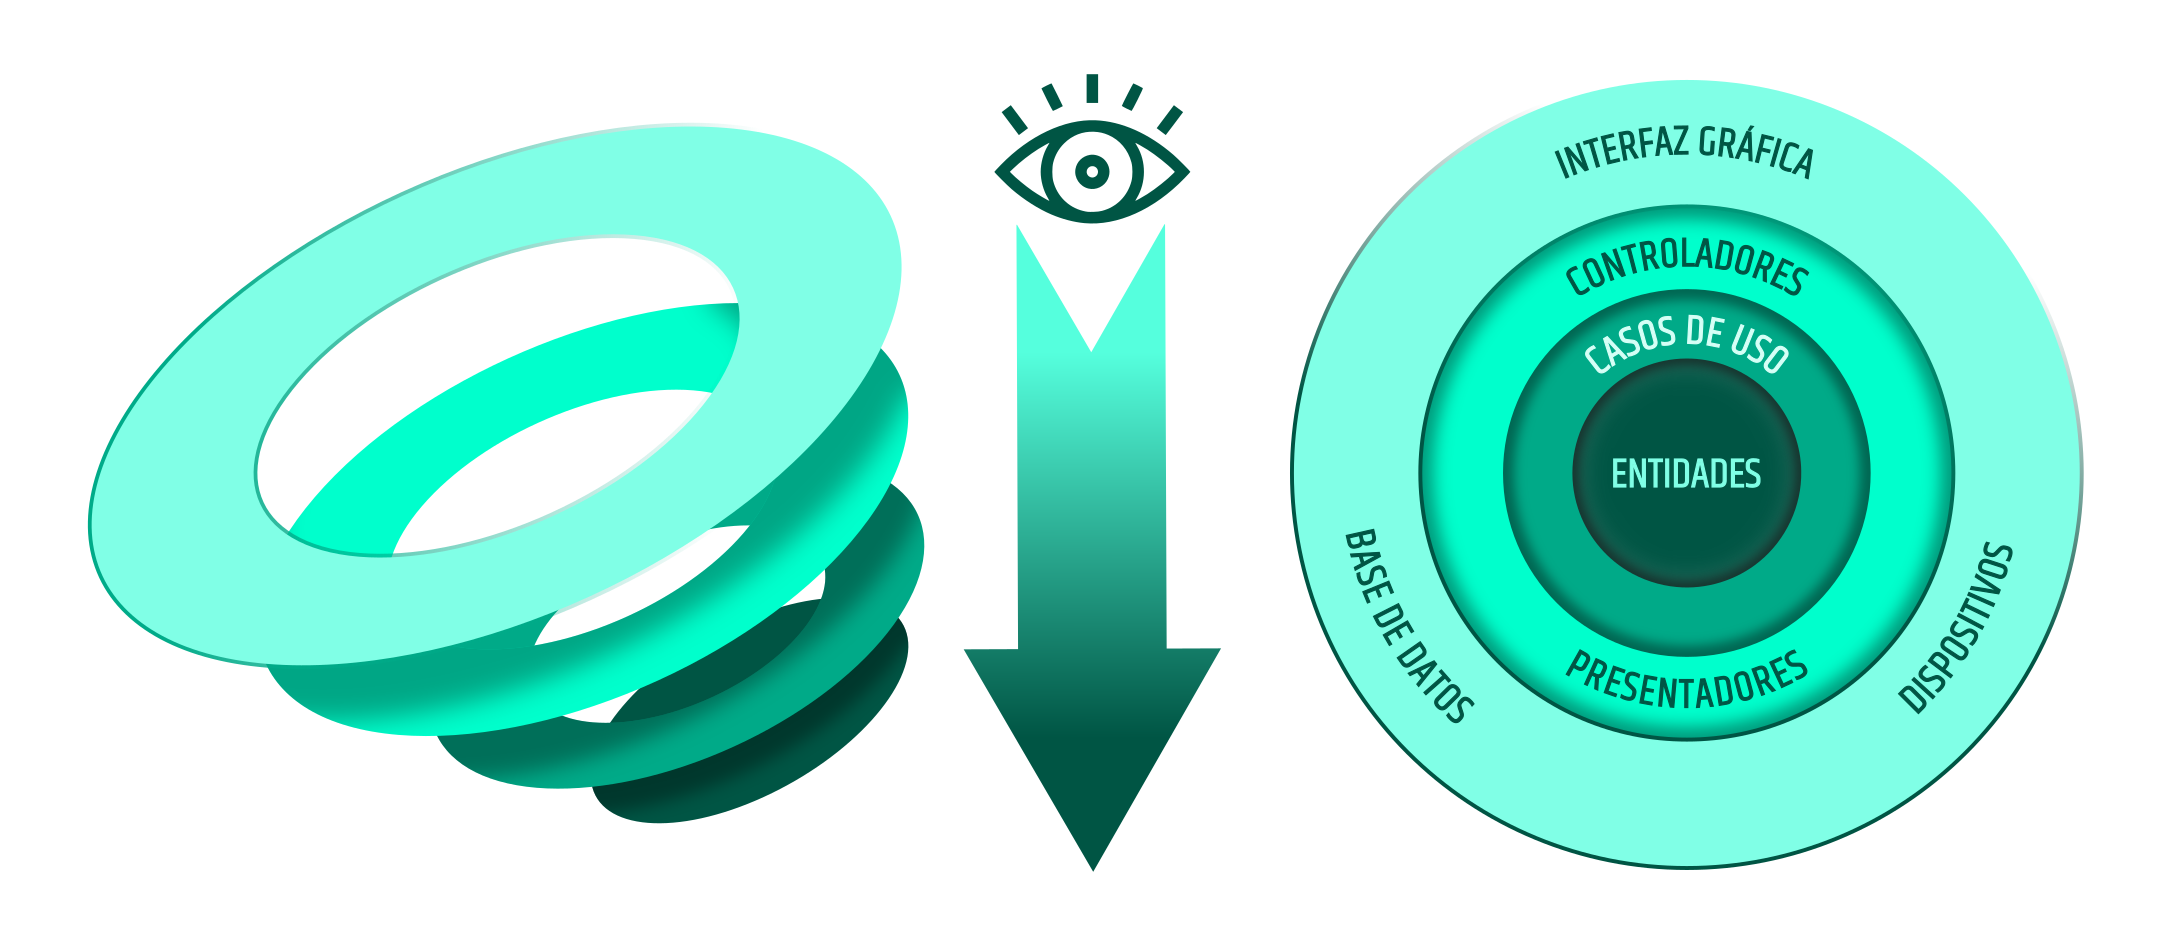
\includegraphics[width=1\textwidth]{Figures/arch_regla_dependencias}
	\rule{35em}{1pt}
	\caption[Principio de Dependecias]{Esquema de dependencias para una arquitectura en capas.}
	\label{fig:Diagrama_clasico}
\end{figure}

\subsubsection{Principio de Abstracción}
El principio de abstracción ya se ha insinuado antes. Postula que, a medida que se recorre el diagrama de la arquitectura de la Figura ~\ref{fig:C2_PA} a lo largo del radio en dirección del centro, las implementaciones se vuelven más abstractas, agnósticas de plataformas y frameworks. Como se mencionó en la sección anterior, el círculo interno contiene lógica de negocios mientras que el exterior comprende los detalles de implementación.

\begin{figure}[htbp]
	\centering
	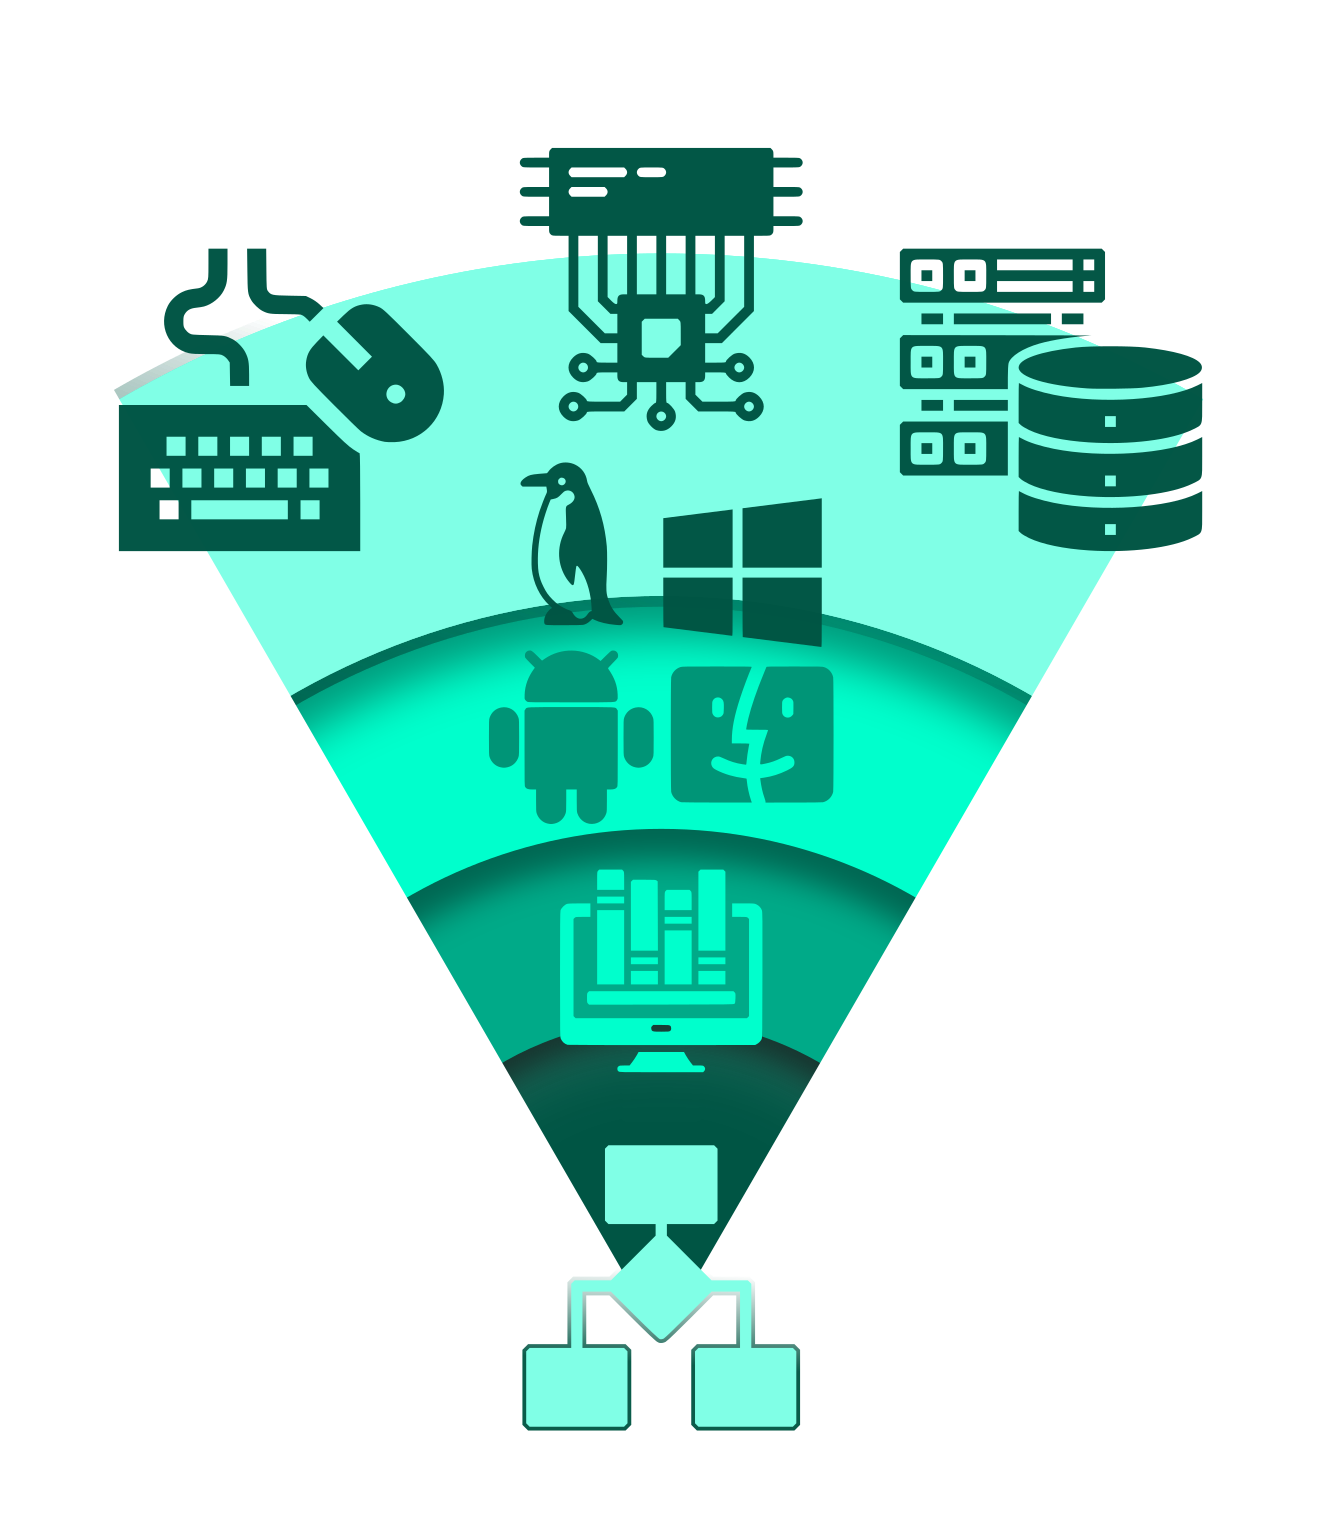
\includegraphics[width=0.5\textwidth]{Figures/arch_regla_abstraccion.png}
	\rule{35em}{1pt}
	\caption[Abstraction Principle]{Principio de Abstracción en una arquitectura por capas.}
	\label{fig:C2_PA}
\end{figure}

\subsubsection{Comunicación entre Capas}
Dado que en esta arquitectura la lógica de negocio se encuentra en el centro del diseño, ésta debe mediar entre los componentes periféricos de entrada y salida.
Aquí se presenta un inconveniente paradójico introducido por el empleo de la regla de dependencias: la capa con lógica de negocios ni siquiera conoce que los componentes en la periferia existen.
Esto representa un desafío ya que necesitamos que los datos sean capaces de fluir desde las capas externas a las internas y viceversa, esto sin violar la regla de dependencias.


Se propone entonces un método para resolver el problema de comunicación entre capas.
En primera instancia se define los objetos \emph{Caso de Uso} como las entidades principales de la Lógica de Negocios.
Se conceptualizan dos puertos para cada caso de uso, uno de entrada y otro de salida.
Mediante el puerto de entrada se reciben parámetros para la ejecución del caso de uso mientras que el puerto de salida permite la extracción de sus resultados.
En la práctica, la definición de estos puertos (interfaces) se realiza dentro de la capa más interna mientras que su implementación e instanciación en la capa más externa. Esto satisface la regla de dependencias y puede visualizarse en la Figura ~\ref{fig:C2_CC_01}.


\begin{figure}[htbp]
	\centering
	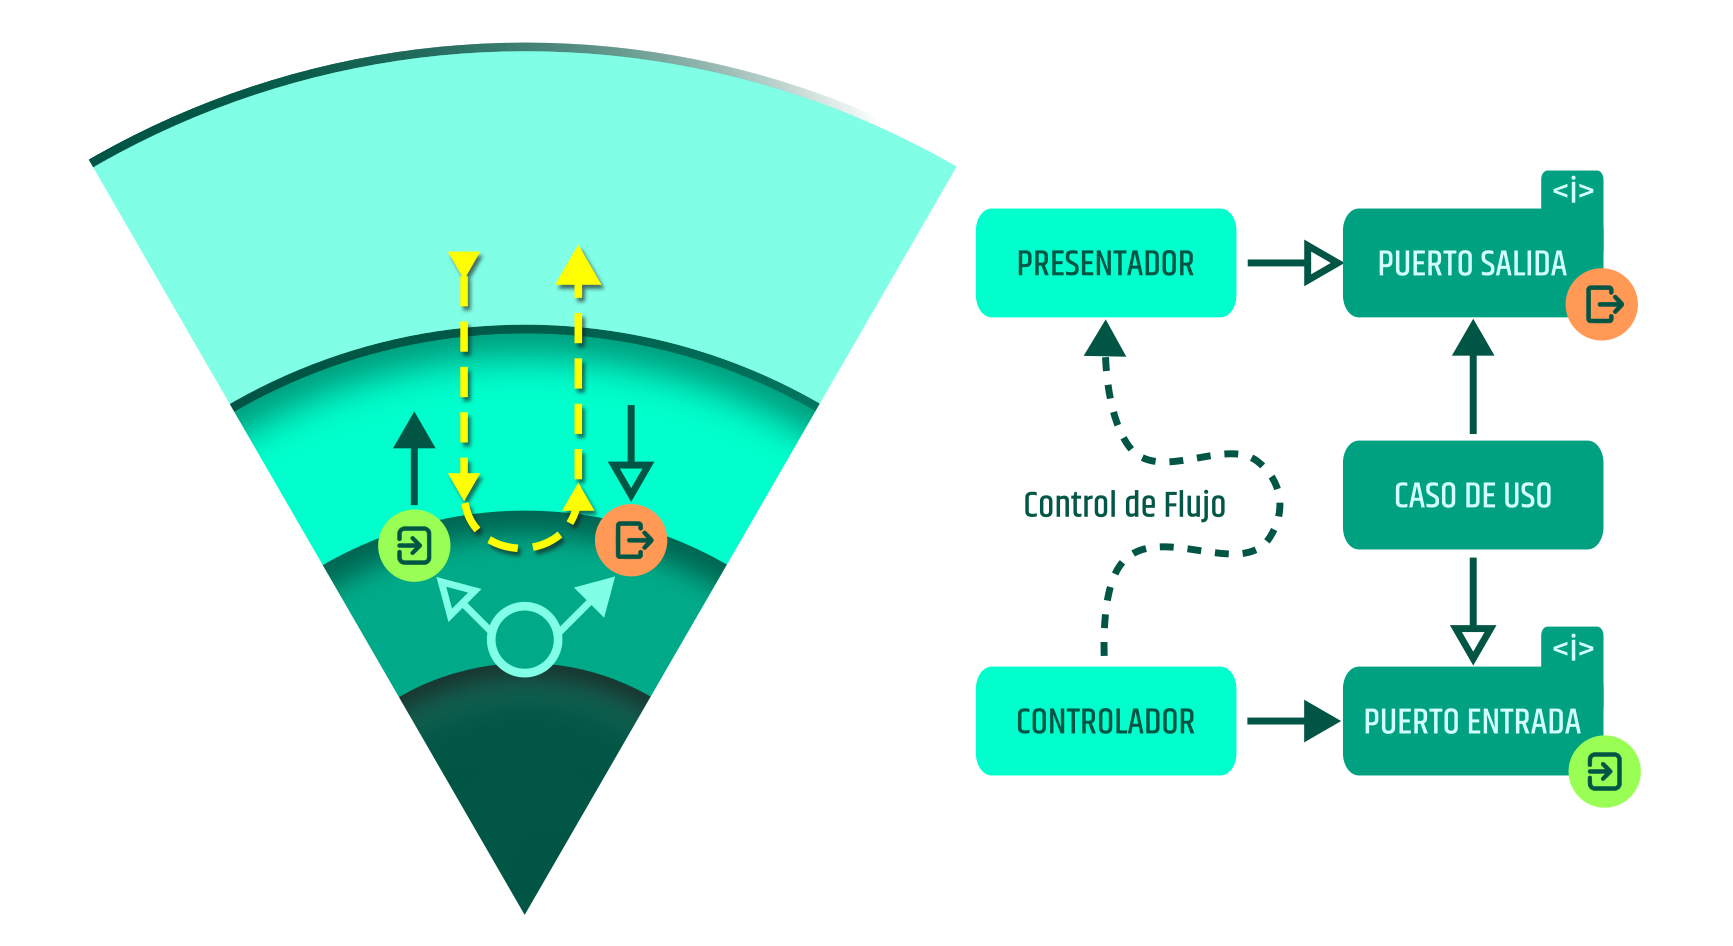
\includegraphics[width=1\textwidth]{Figures/arch_comunicacion_capas.png}
	\rule{35em}{1pt}
	\caption[Layer Communication]{Comunicación entre capas.}
	\label{fig:C2_CC_01}
\end{figure}


\section{Diseño de Capas}
Como parte del proyecto de PPS se investigaron implementaciones reales de esta arquitectura en proyectos android.
Las dos mejores disponibles a código abierto y con buena documentación pertenecen a un desarrollador argentino Fernando Cejas \cite{clean_cejas} (SoundCloud) y al repositorio de Blueprints Arquitectónicos de Google\cite{clean_android_blueprints}.\\
Ambas propuestas dividen la implementación en tres capas principales, una capa de presentación, una capa de dominio y la capa de datos.
Cada capa tiene una responsabilidad bien definida y se comunica con una única capa vecina respetando la regla de dependencias.
La cadena de comunicación puede apreciarse en la figura ~\ref{fig:Diagrama_clasico2}. La capa de presentación transmite las acciones del usuario a la capa de dominio, la cual efectúa solicitudes de información a la capa de datos. Una vez resueltas, la capa de datos enviará los resultados de vuelta a la capa de dominio que ejecutará la lógica de negocios correspondiente. Esto genera una respuesta que, a su vez, produce los efectos deseados en la capa de presentación.\\
\begin{figure}[htbp]
	\centering
	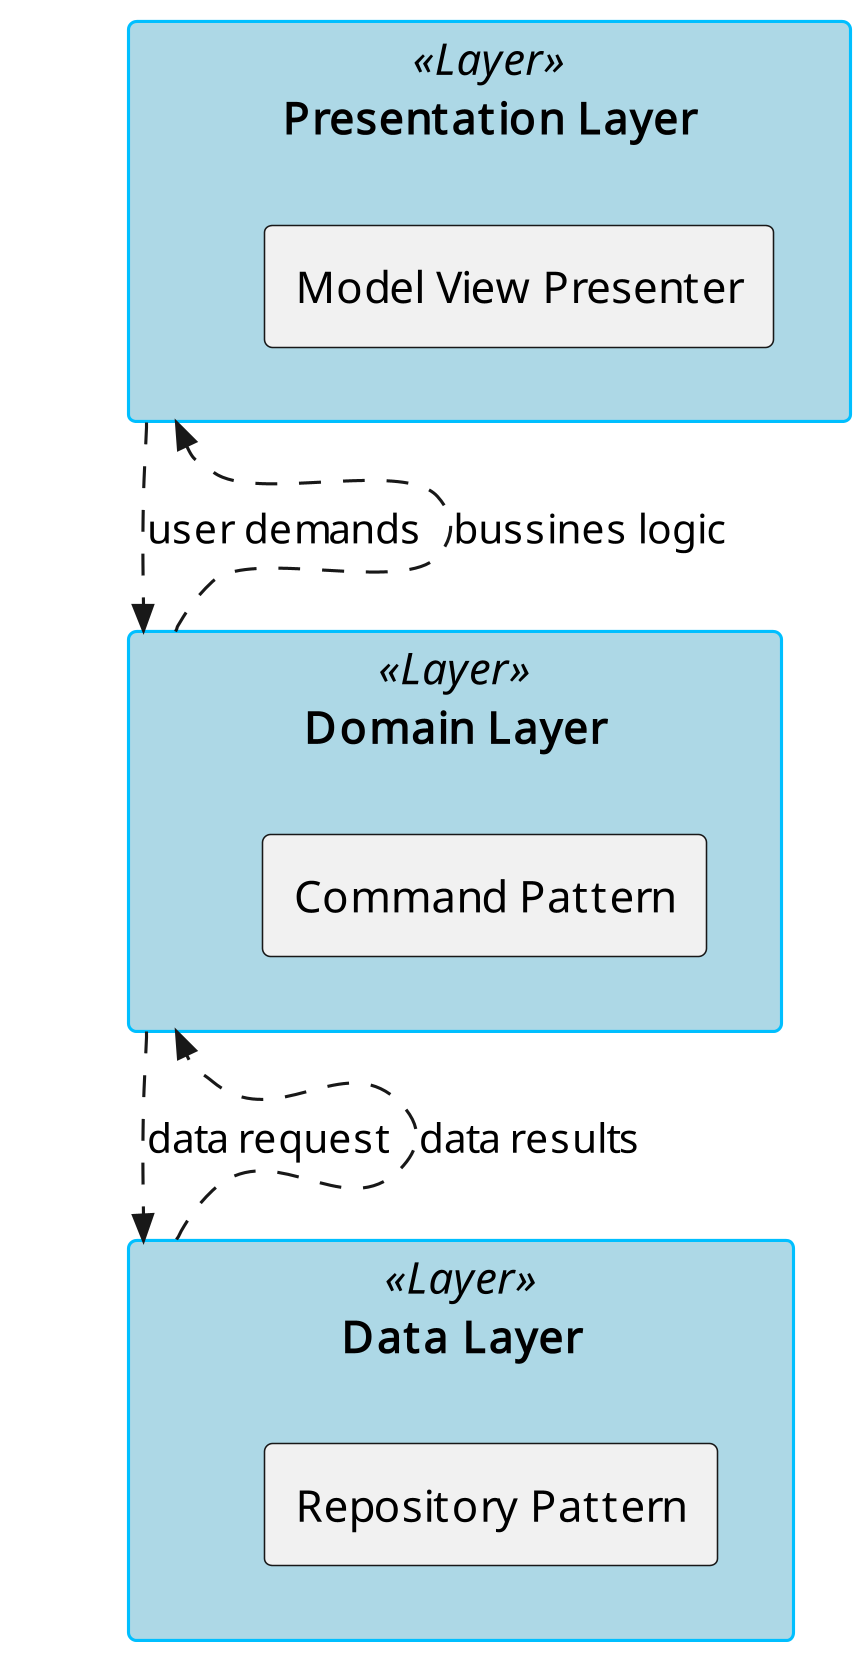
\includegraphics[width=0.3\textwidth]{Figures/design/FLOW_clean.png}
	\rule{35em}{1pt}
	\caption[Dependencia de Módulos]{Diagrama de Flujo de Información entre las capas de la arquitectura..}
	\label{fig:Diagrama_clasico2}
\end{figure}
A continuación se describe brevemente las responsabilidades de cada capa.


\begin{itemize}
	\item Capa de Presentación: Esta capa se encarga de presentar la interfaz de usuario, esto es, mostrar por pantalla los objetos visuales correspondientes y recibir los eventos de interacción que realiza el usuario. Para la implementación se recomienda el empleo del patrón de diseño conocido como \textbf{MVP (Model View Presenter)}. 
	\item Capa de Dominio: Esta capa contiene toda la lógica de negocio. La capa de dominio contiene las clases denominadas casos de uso o interactores según la literatura. Estos objetos encapsulan los escenarios contemplados por la lógica de negocio y son ejecutados por la capa de presentación. Estos casos de uso representan todas las acciones posibles admitidas por el sistema y que pueden ser compuestas en la implementación por los desarrolladores siempre desde la capa de presentación. Para la implementación de estos casos de uso se sugiere la utilización del patrón de diseño conocido como \textbf{Command Pattern}.
	\item Capa de Datos: Esta capa administra la adquisición de datos y es capaz de utilizar diferentes orígenes de datos, así como la lógica de cache o persistencia temporal. Esta capa se suele implementar utilizando el patrón de diseño conocido como \textbf{Repository Pattern}.  
\end{itemize}
\subsection{Capa de Presentación: Model View Presenter (MVP)}
El patrón de arquitectura que se utiliza en la capa de presentación se conoce como Modelo-Vista-Presentador.
La idea detrás del patrón es concentrar la interacción con el usuario en una entidad conocida como presentador, las operaciones directamente relacionadas con la manipulación de objetos gráficos y la captura de acciones de usuario están delegadas a la entidad Vista, finalmente la adquisición de datos y la ejecución de los algoritmos que encapsulan la lógica de negocio forman parte de las entidades modelo en el patrón \cite{mvp_leiva}.
El diagrama de componentes ~\ref{fig:uml_mvp_component} describe la relación entre los objetos principales.


\begin{figure}[htbp]
	\centering
	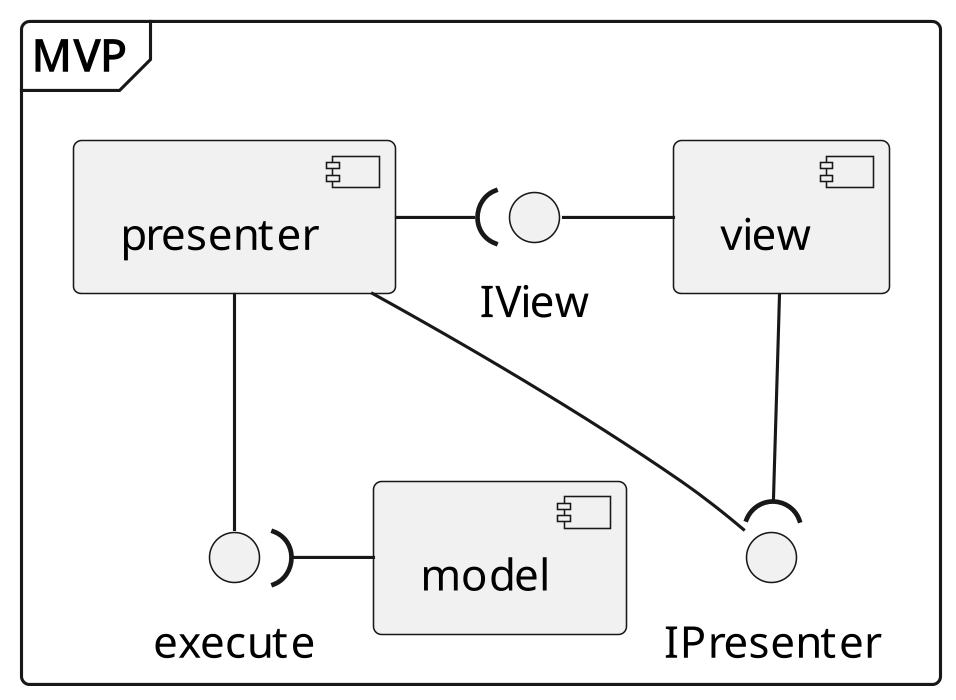
\includegraphics[width=0.5\textwidth]{Figures/design/COMP_mvp.png}
	\rule{35em}{1pt}
	\caption[MVP Components]{Diagrama de componentes del patrón.}
	\label{fig:uml_mvp_component}
\end{figure}

Es posible deducir el modo en que interactúan los componentes. El presentador se comunica de manera bidireccional con la vista y de manera unidireccional con el modelo.

Una convención para la implementación del patrón es tratar de generar vistas completamente ajenas de cualquier lógica operativa y agnósticas del estado de la aplicación. Esto las convierte en un mero instrumento de interfaz entre lo que percibe el usuario y sus reacciones. 

Otra de las convenciones sugiere utilizar objetos modelo-vista en la comunicación entre el presentador y la vista para estandarizar el tipo de mensaje y el proceso de actualización de la vista.

En el caso de las implementaciones antes mencionadas la interfaz con el modelo es satisfecha mediante el uso de objetos casos de uso ó interactores, ambos términos suelen utilizarse de manera intercambiable.

La secuencia de mensajes que son intercambiados entre los objetos del patrón se ilustran en el diagrama de secuencias ~\ref{fig:uml_mvp_sequence}

\begin{figure}[htbp]
	\centering
	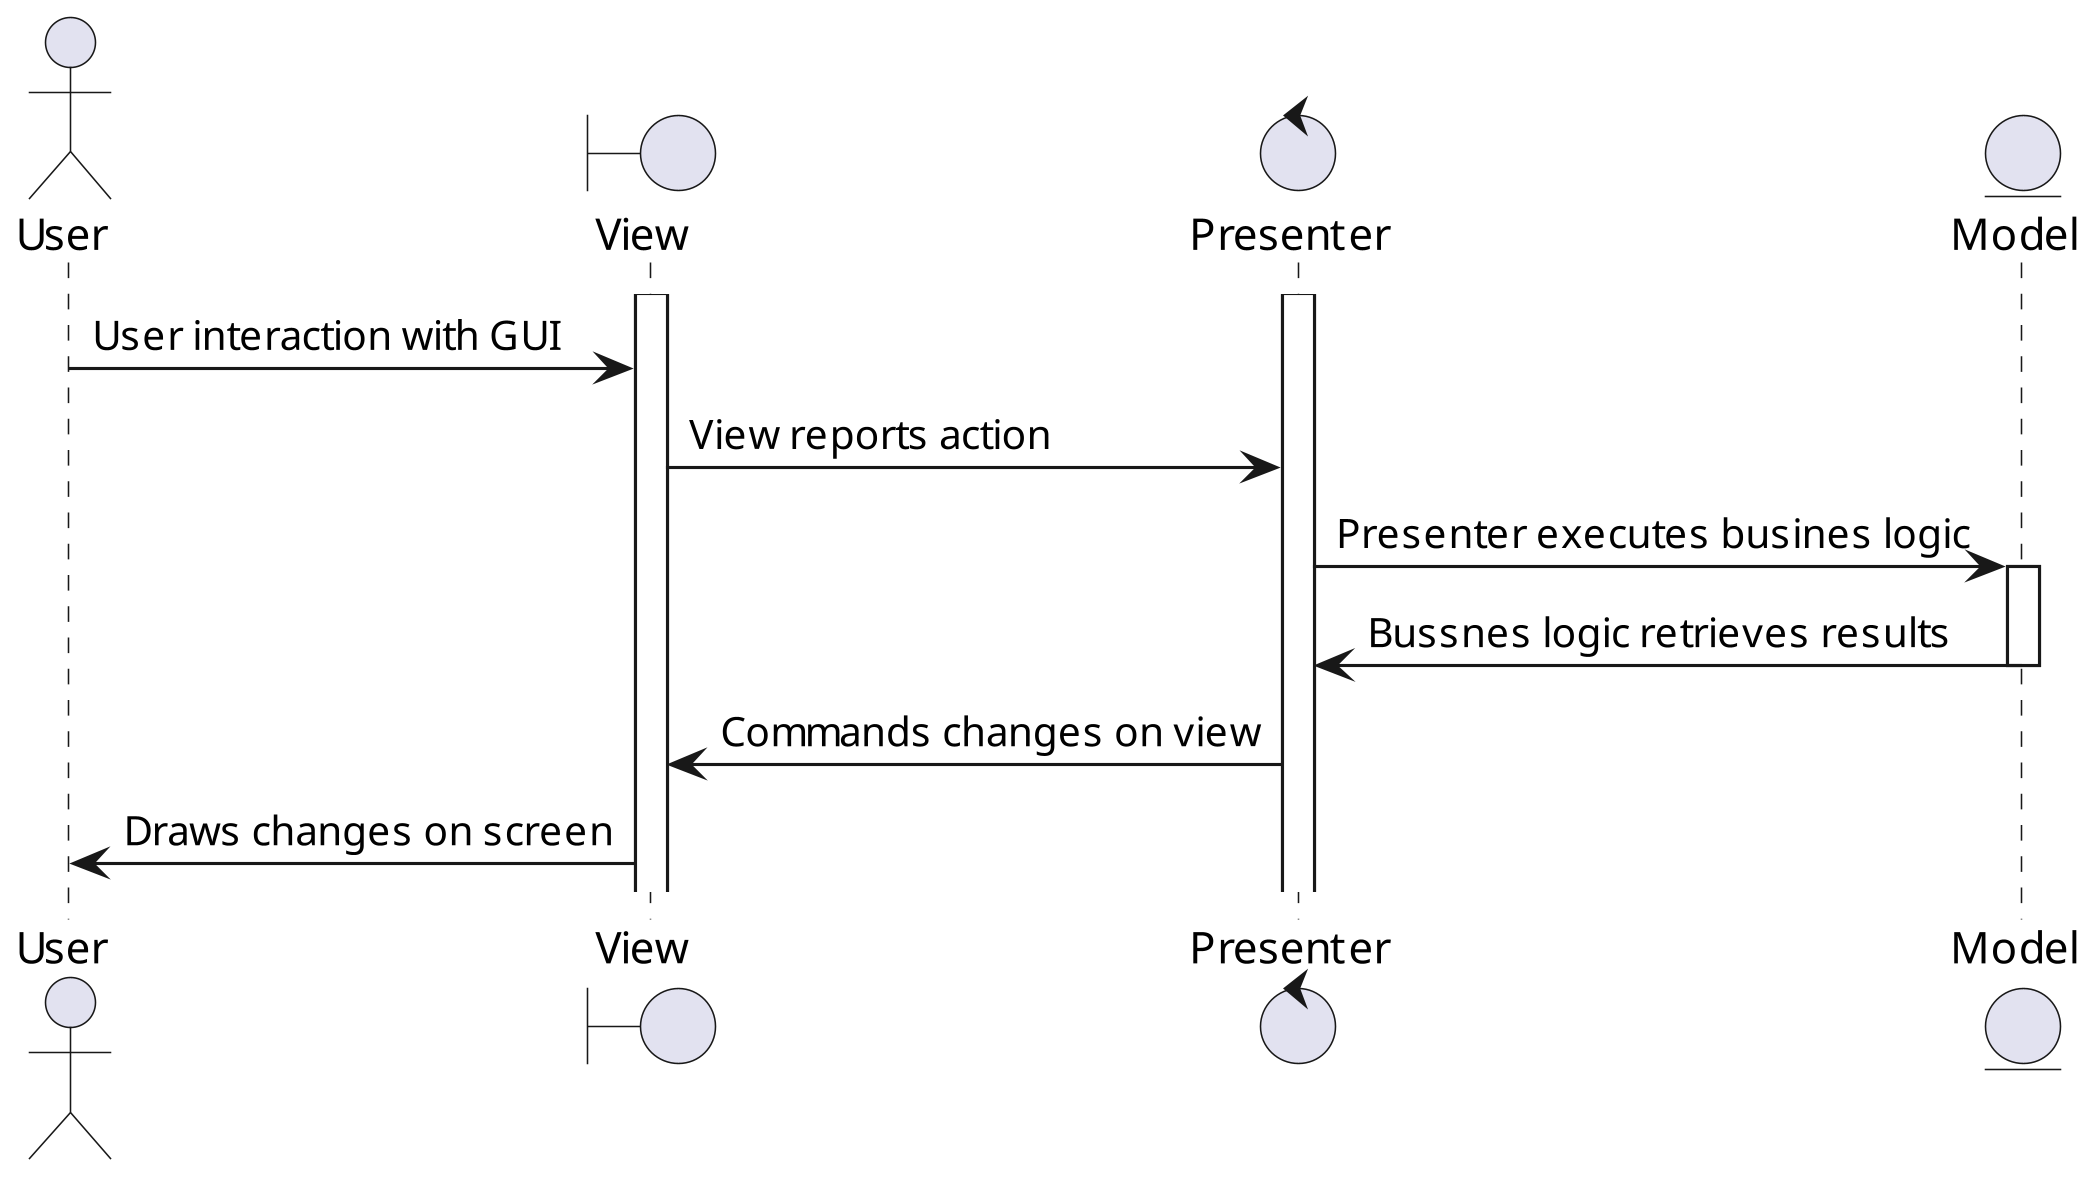
\includegraphics[width=0.7\textwidth]{Figures/design/SEQ_mvp.png}
	\rule{35em}{1pt}
	\caption[MVP Sequence]{Diagrama de secuencia para una interacción con el usuario utilizando MVP.}
	\label{fig:uml_mvp_sequence}
\end{figure}


\subsection{Capa de Dominio: Patrón Command}
El patrón de diseño \emph{Command} se utiliza para abstraer la ejecución de procedimientos mediante la implementación de entidades comando \cite{comm_sugrue}. Estos objetos ejecutan un único algoritmo y encapsulan la lógica de negocio de la aplicación o sistema.
Originalmente el diseño contempla 4 entidades principales que se pueden apreciar en el diagrama de clases de la figura ~\ref{fig:uml_clases_commander}:

\begin{figure}[htbp]
	\centering
	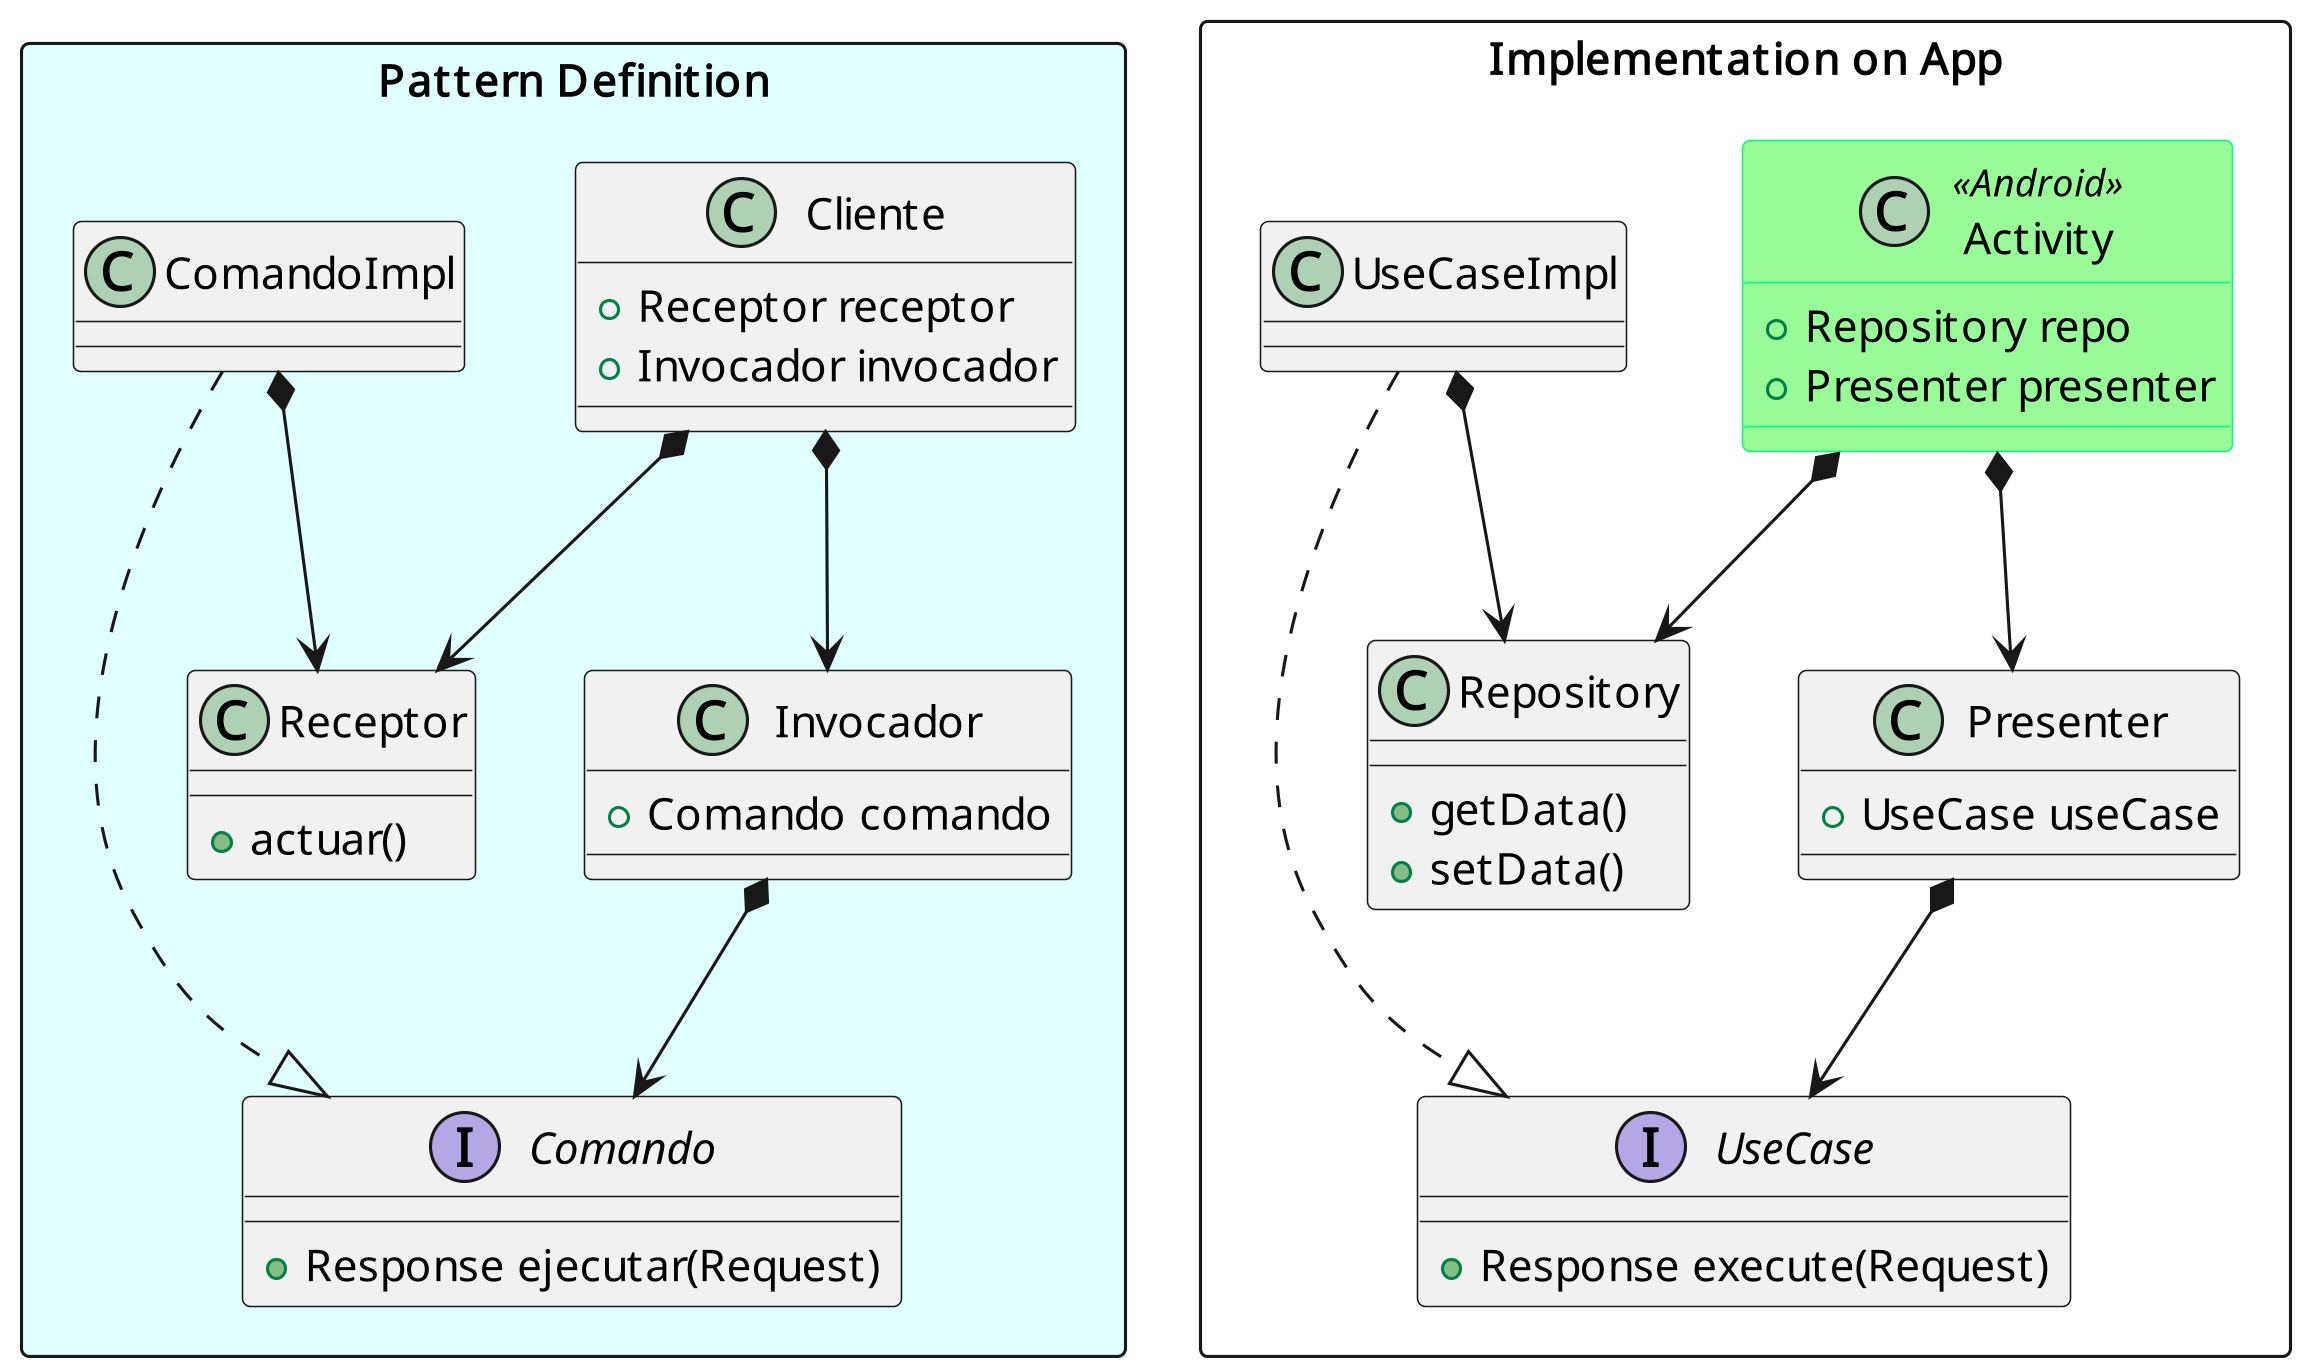
\includegraphics[width=0.8\textwidth]{Figures/design/CLASS_command_versus.png}
	\rule{35em}{1pt}
	\caption[Commander Classes]{Diagrama de clases para el planteo inicial del patrón Command y su adaptación para este proyecto.}
	\label{fig:uml_clases_commander}
\end{figure}

\begin{enumerate}
	\item Cliente: Este componente se encarga de crear las instancias de cada comando y distribuirlas entre los correspondientes invocadores.
	\item Receptor: Es la entidad que se ve afectada por la ejecución de un comando. Puede ser compartida por varios comandos o bien un único comando puede interactuar con varios receptores en su ejecución.
	\item Comando: Es el objeto que contiene la implementación del algoritmo o lógica de ejecución.
	\item Invocador: Se encarga de ejecutar instancias de comandos.
\end{enumerate}

\begin{figure}[htbp]
	\centering
	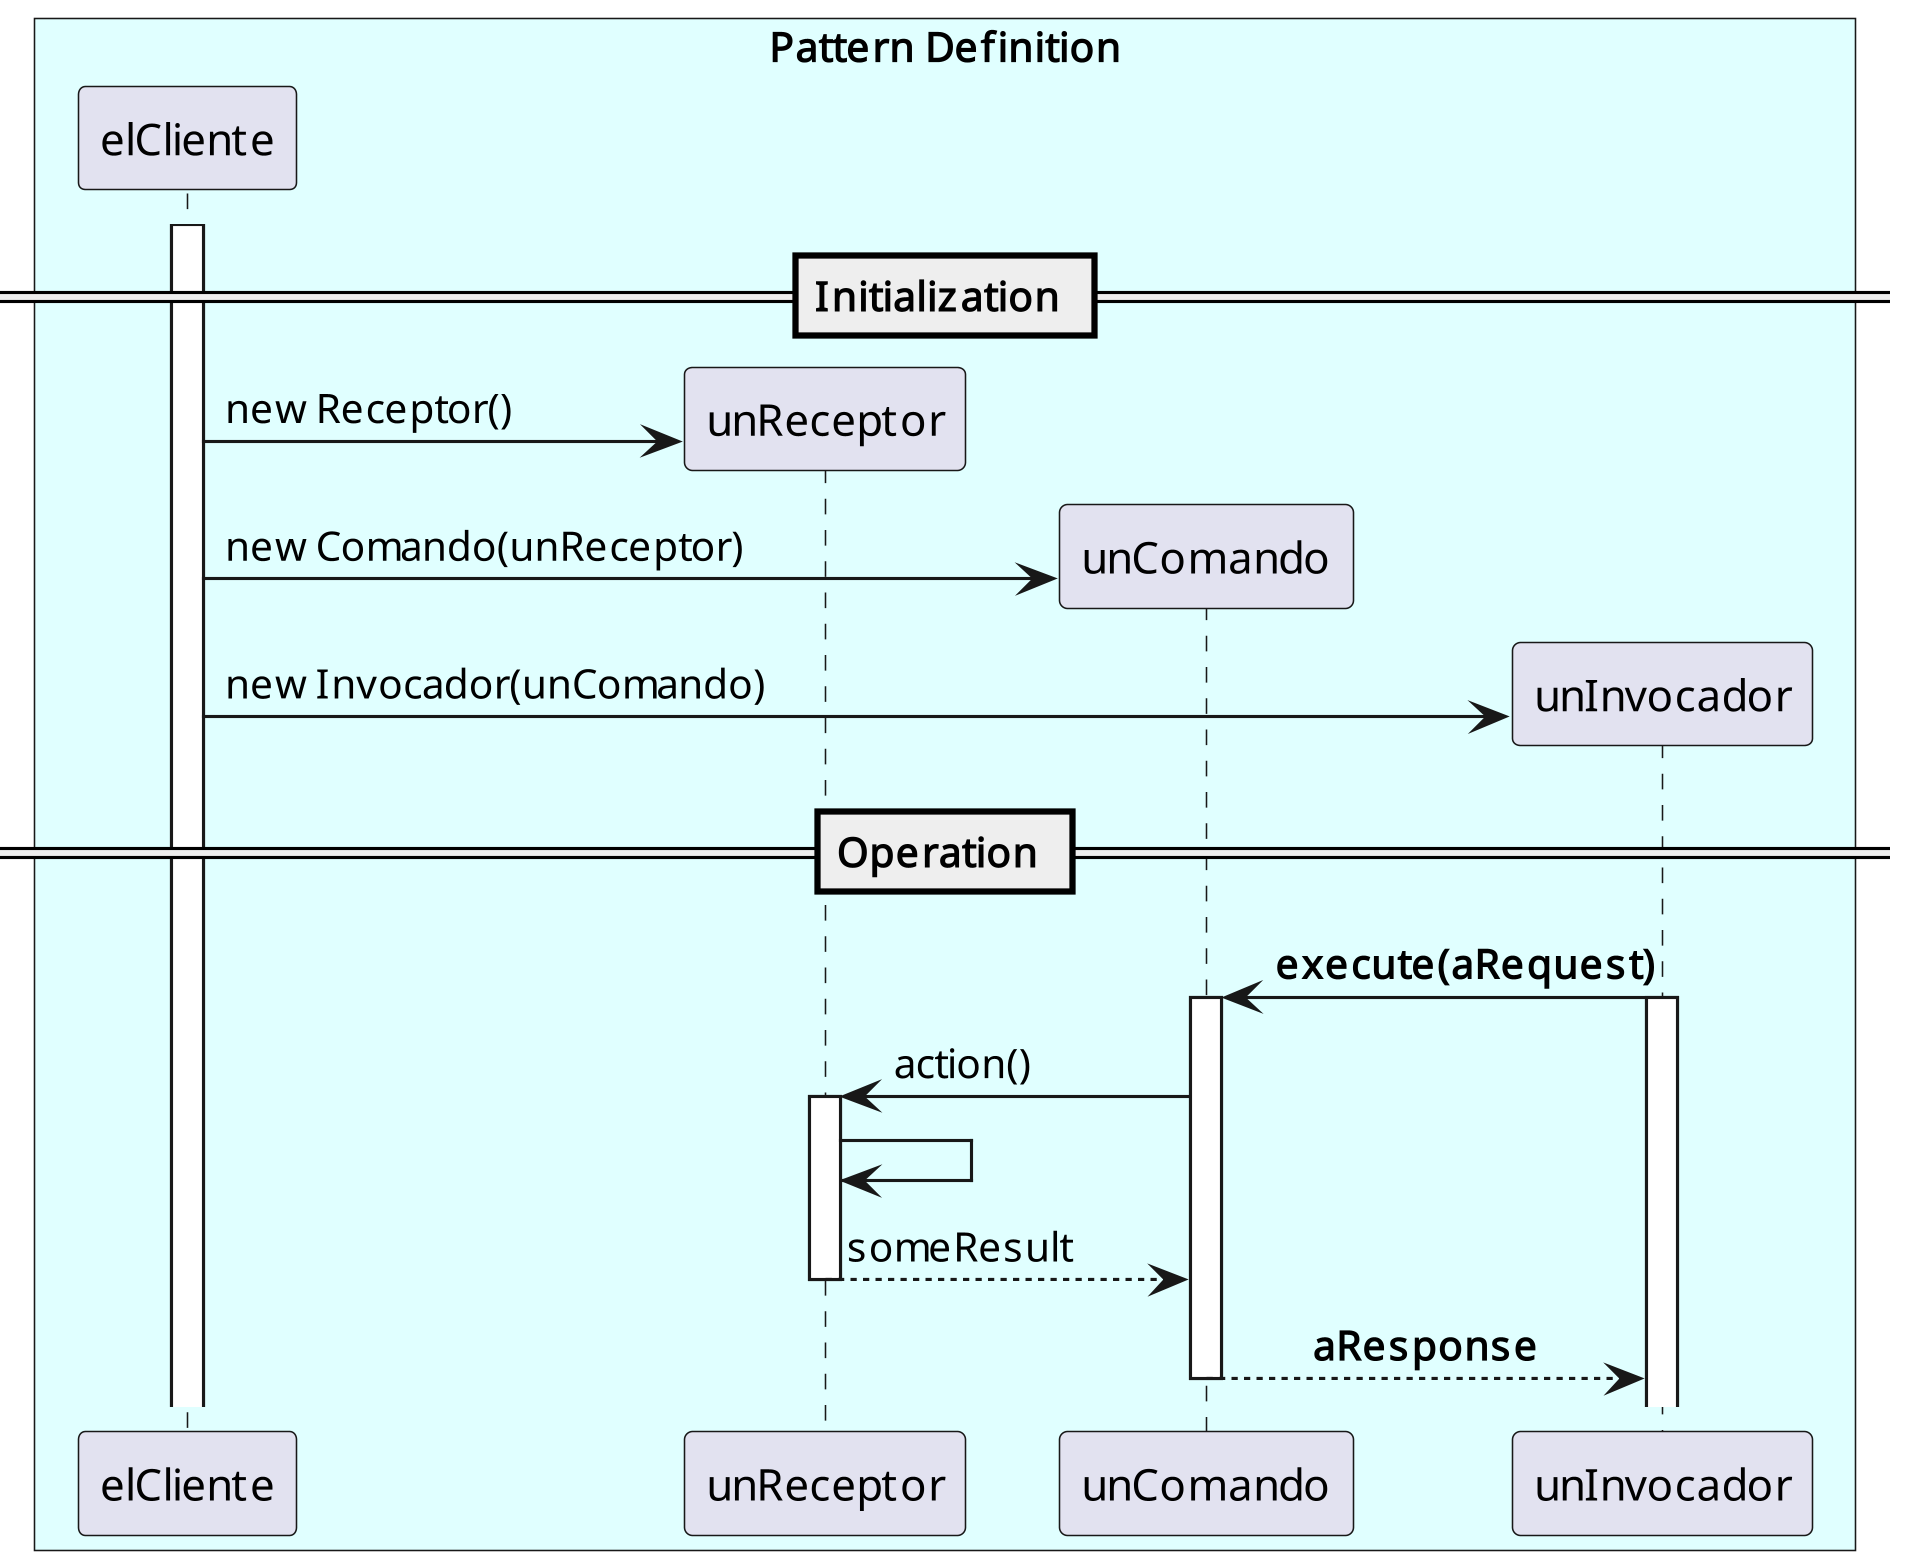
\includegraphics[width=0.8\textwidth]{Figures/design/SEQ_command_def_req_resp.png}
	\rule{35em}{1pt}
	\caption[MVP Components]{Diagrama de secuencia para el patrón Commander.}
	\label{fig:uml_commander_sequence}
\end{figure}

La mayoría de los ejemplos de aplicación de este patrón implementan un comando
por cada una de las operaciones soportadas por el sistema o aplicación. Sin embargo en sistemas suficientemente grandes la diversidad de funcionalidades soportadas es tal que el diseño propuesto se vuelve impráctico.
Para mitigar este problema se suele implementar de manera adicional una modificación que permite la ejecución paramétrica de los comandos para reducir al máximo la cantidad de comandos implementados.
Esta modificación permite diversas alternativas de implementación pero la más utilizada incorpora  conceptos del patrón Request-Response dónde el comando es utilizado como un objeto tipo caja negra que admite Solicitudes y emite Respuestas estandarizadas para cada caso.
\begin{itemize}
	\item Solicitud (Request): Un objeto que contiene el conjunto de parámetros de entrada que deben ser satisfechos para poder realizar la ejecución de la rutina del comando.
	\item Respuesta (Response): Un objeto que contiene los valores que se obtuvieron de la ejecución del algoritmo del comando.
\end{itemize}

Teniendo en cuenta estos detalles se describe el flujo de operación y ejecución ~\ref{fig:uml_commander_sequence_req_resp} de un comandos:

\begin{enumerate}
	\item El cliente crea instancias de comandos y sus correspondientes invocadores. 
	\item El invocador crea e inicializa los objeto solicitud necesarios para ejecutar cada comando.
	\item El invocado ejecuta los comandos llamando al método ''ejecutar'' implementado por cada comando pasando como parámetro la solicitud previamente creada.
	\item El invocador observa los resultados en espera activa implementando el patrón Observer o mediante algún esquema de callback.
\end{enumerate}



\begin{figure}[htbp]
	\centering
	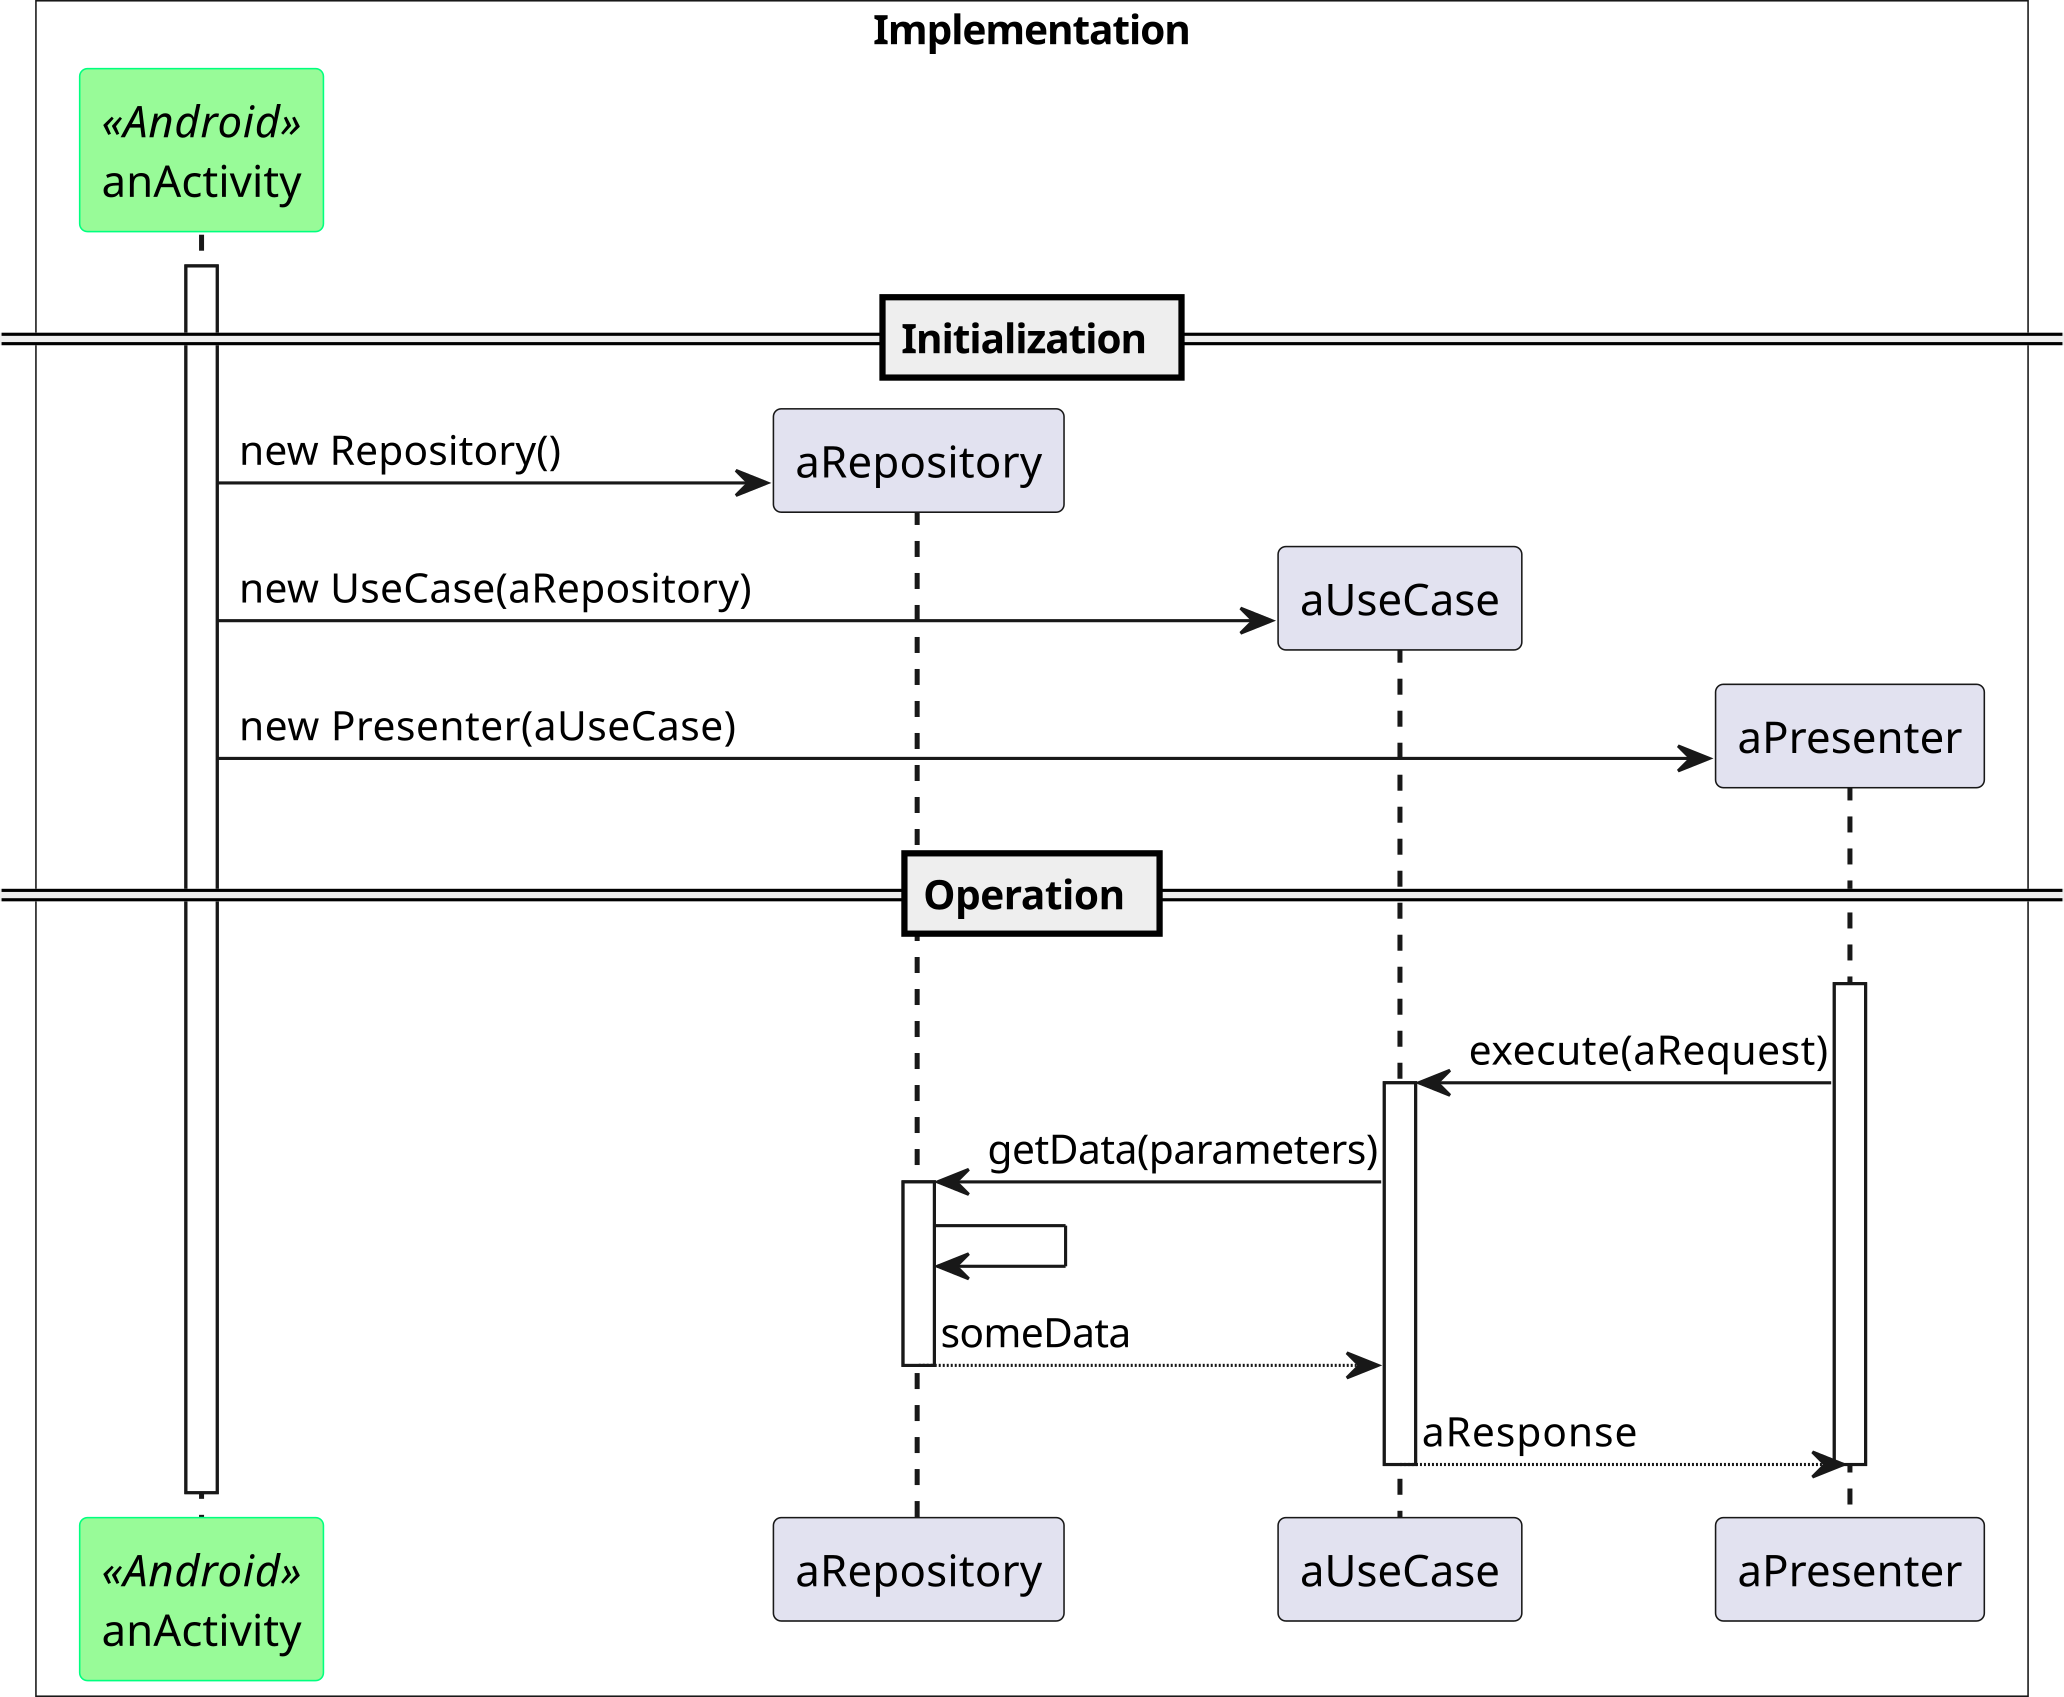
\includegraphics[width=0.8\textwidth]{Figures/design/SEQ_command_app.png}
	\rule{35em}{1pt}
	\caption[Commander Review]{Diagrama de secuencia para el diseño revisado.}
	\label{fig:uml_commander_sequence_req_resp}
\end{figure}

Siguiendo los lineamientos de la arquitectura propuesta los autores denominan a los comandos: Casos de Uso, ó Interactores.

Como una nota relevante de implementación se recomienda ejecutar las rutinas de los comandos en un hilo/proceso separado para evitar bloquear el proceso principal de la aplicación.

\subsection{Capa de Datos: Patrón Repository}
\label{section:repository}
En la capa de datos se propone la implementación de un patrón de diseño conocido como Repository(Repositorio). 
Originalmente se concibe a este diseño como una forma de estandarizar la implementación y el uso de los objetos DAO (Data Access Object) comúnmente utilizados para mapear objetos entidad con las persistencias en la base de datos \cite{repo_wolf}.
Adicionalmente este patrón encapsula en la clase repositorio todos los métodos particulares de filtrado, procesamiento calculado y ordenamiento de entidades.
Sin embargo se define una interfaz genérica que deberá ser respetada por todas las implementaciones de repositorios para todo el sistema independientemente de la entidad que atienda.
En el diagrama de clases de la figura ~\ref{fig:uml_clases_repository} se puede apreciar el diseño original del patrón.

\begin{figure}[htbp]
	\centering
	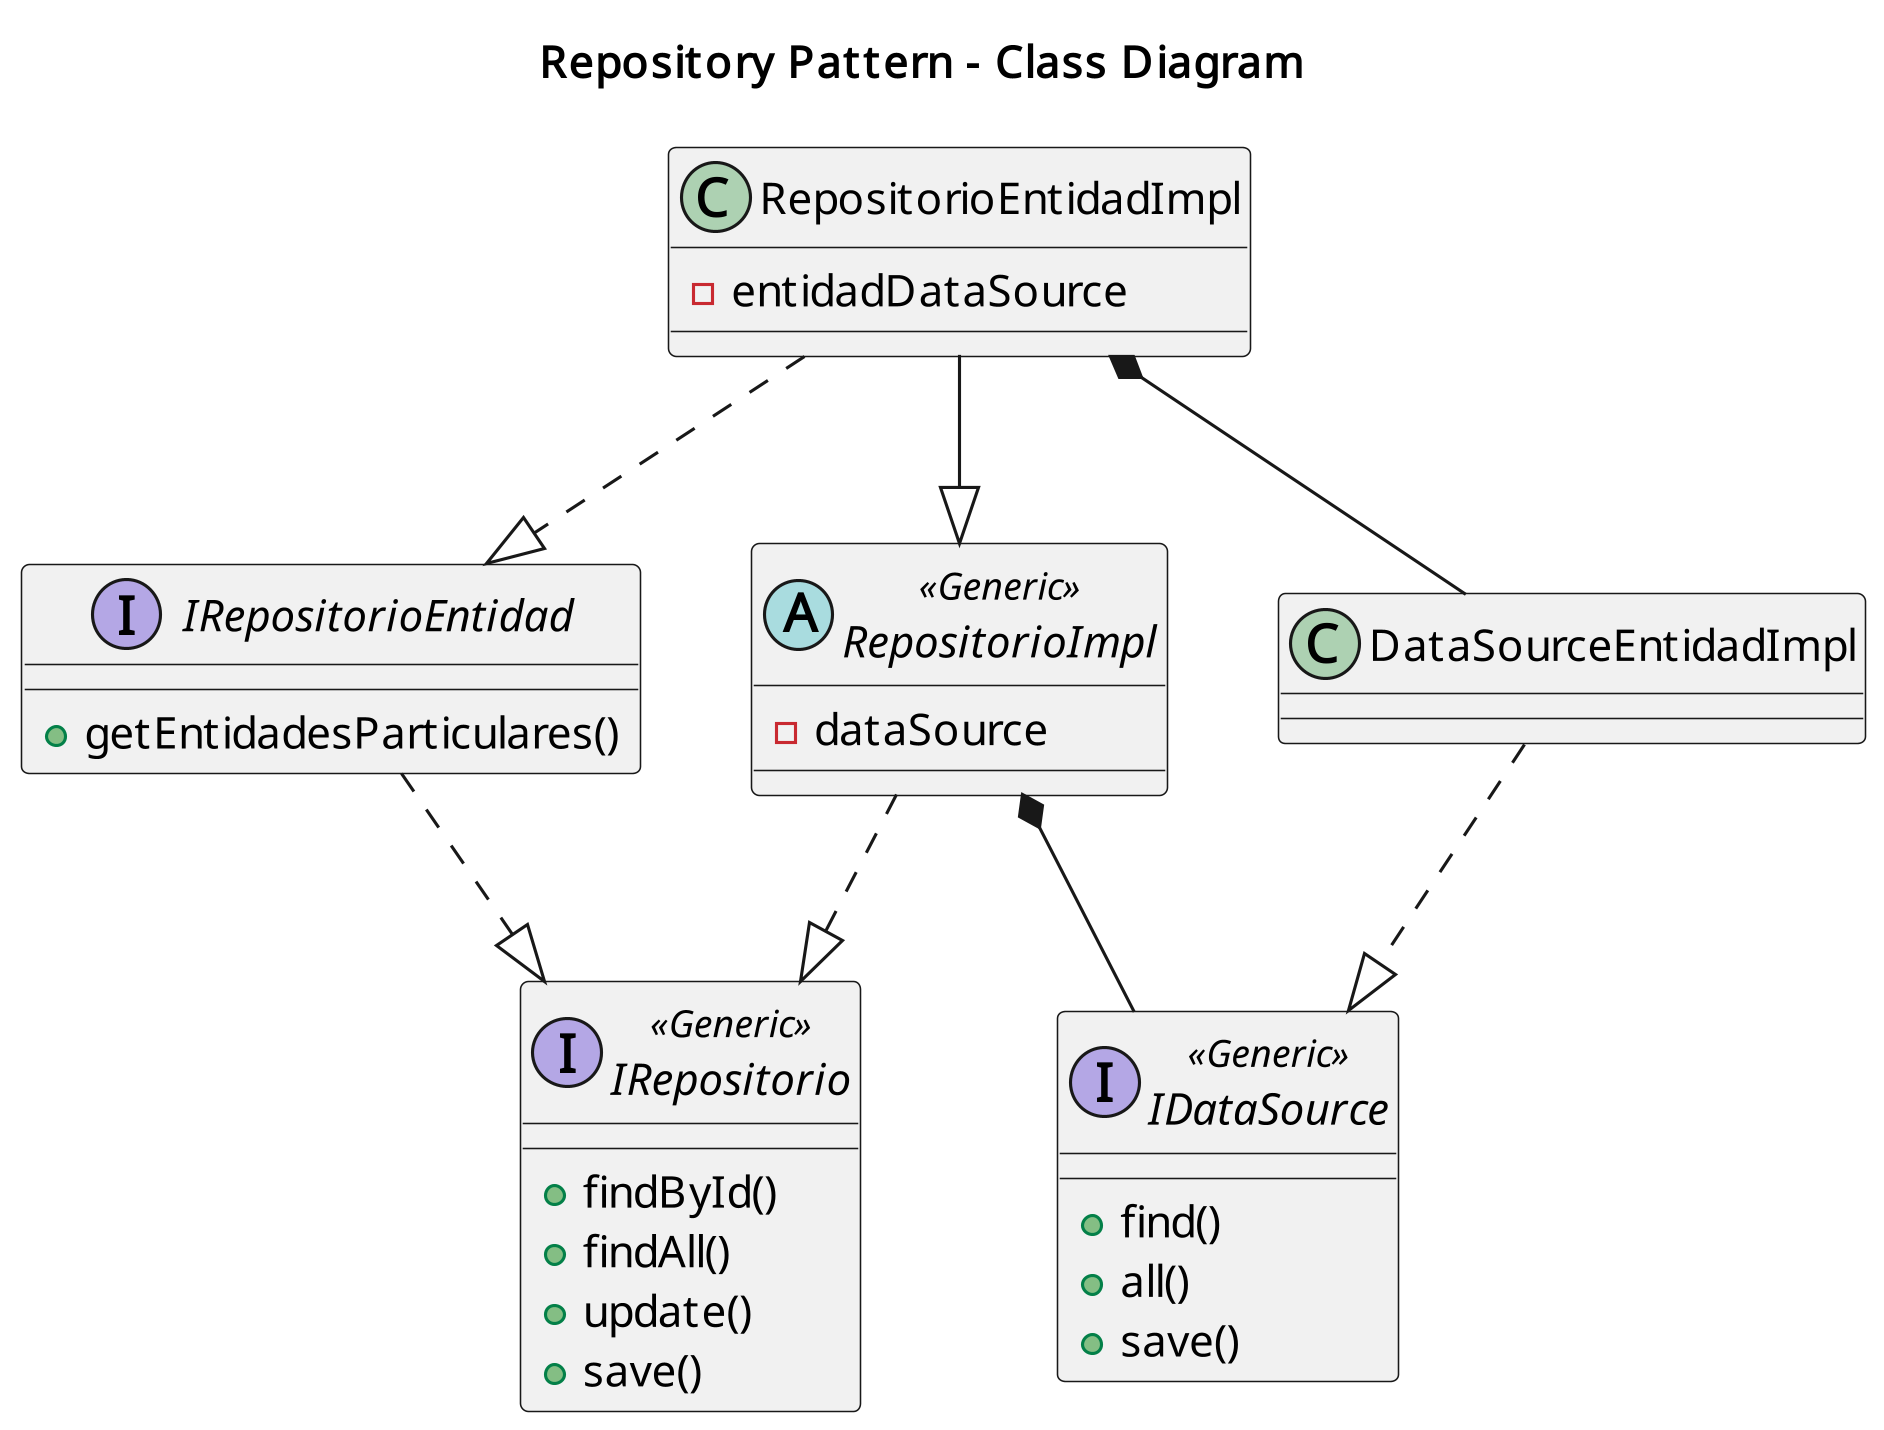
\includegraphics[width=0.8\textwidth]{Figures/design/CLASS_repository_def.png}
	\rule{35em}{1pt}
	\caption[Repository Pattern Class Diagram]{Diagrama de clases del patrón Repository.}
	\label{fig:uml_clases_repository}
\end{figure}

Como puede apreciarse en el diagrama se definen:
\begin{itemize}
	\item IRepositorio: es una interfaz genérica que establece el contrato básico que deben respetar todas las implementaciones de repositorios.
	\item RepositorioImpl: es una clase genérica que establece la interacción con una fuente de datos genérica.
	\item IRepositorioEntidad: es la interfaz que \textit{Especifica} la interfaz genérica de repositorio y establece el contrato o métodos particulares que deberá cumplir la implementación concreta de repositorio para esta Entidad en particular.
	\item RepositorioEntidadImpl: es la clase que \textit{Especifica} la implementación genérica de repositorio e implementa los métodos particulares para esta Entidad en particular.
\end{itemize}

En una repaso más detallado del diagrama puede observarse que existen dos interfaces genéricas para acceso de datos IRepository y IDataSource, esto podría generar confusión y duplicación de código. Adicionalmente en cualquier implementación moderna de sistemas con persistencia es prácticamente mandatario el empleo de frameworks que soportan ORM (Object Relational Mapping) out-of-the-box.
En la figura ~\ref{fig:uml_clases_detalles_repository} se puede observar la modificación sobre la propuesta original del patrón de diseño.

\begin{figure}[htbp]
	\centering
	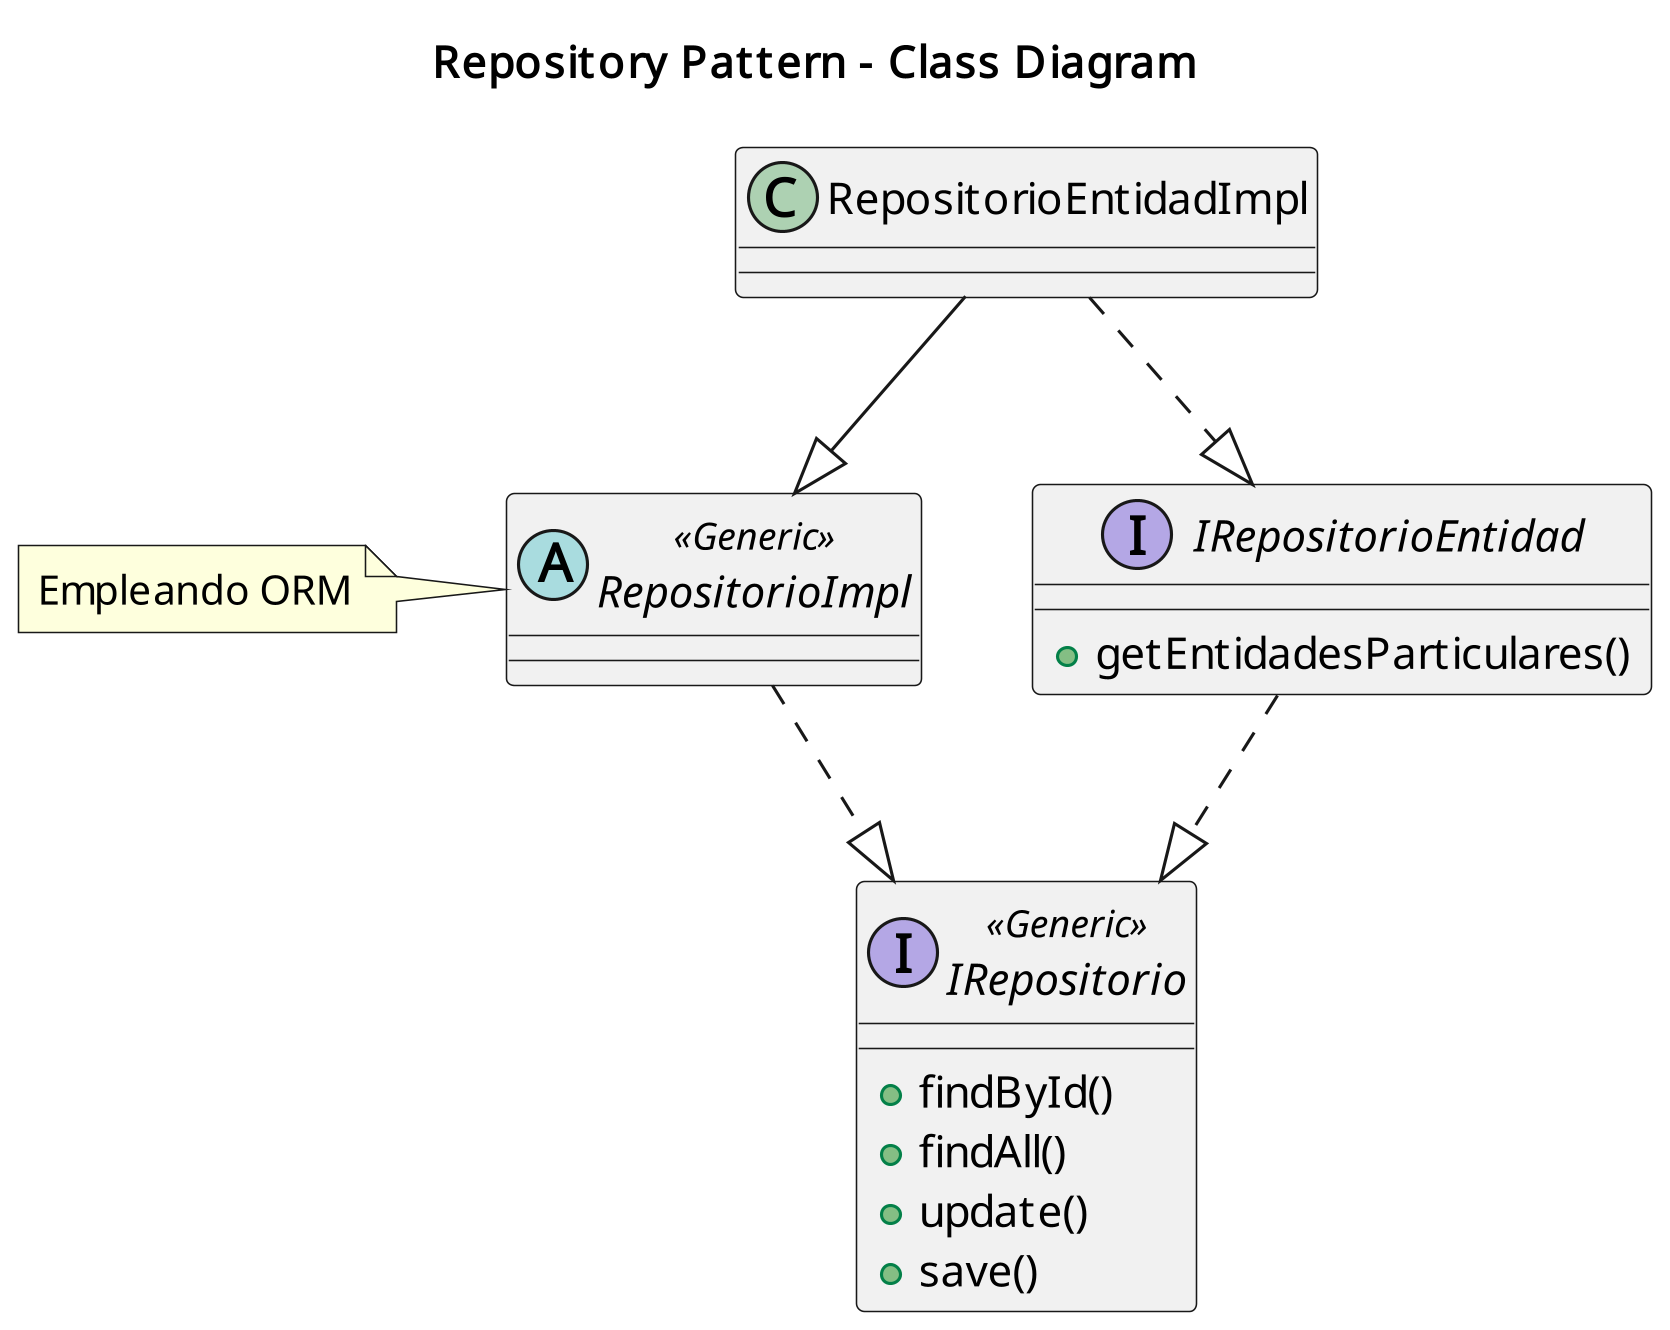
\includegraphics[width=0.8\textwidth]{Figures/design/CLASS_repository_less.png}
	\rule{35em}{1pt}
	\caption[Repository Pattern Detailed Class Diagram]{Diagrama de clases reducido del patrón Repository.}
	\label{fig:uml_clases_detalles_repository}
\end{figure}

En las implementaciones mencionadas se reemplaza la interfaz del repositorio por la interfaz fuente de datos. Coloquialmente es fácil de entender ya que un repositorio definitivamente es una fuente de datos. Si además se quita la estandarización por genéricos se consigue un diseño más sencillo y que genera menos código estructural o scafold manteniendo un único contrato o interfaz de acceso a los datos. En la figura ~\ref{fig:uml_clases_modif_repository} se puede observar la modificación mencionada y el diseño final propuesto para la implementación del patrón.

 \begin{figure}[htbp]
	\centering
	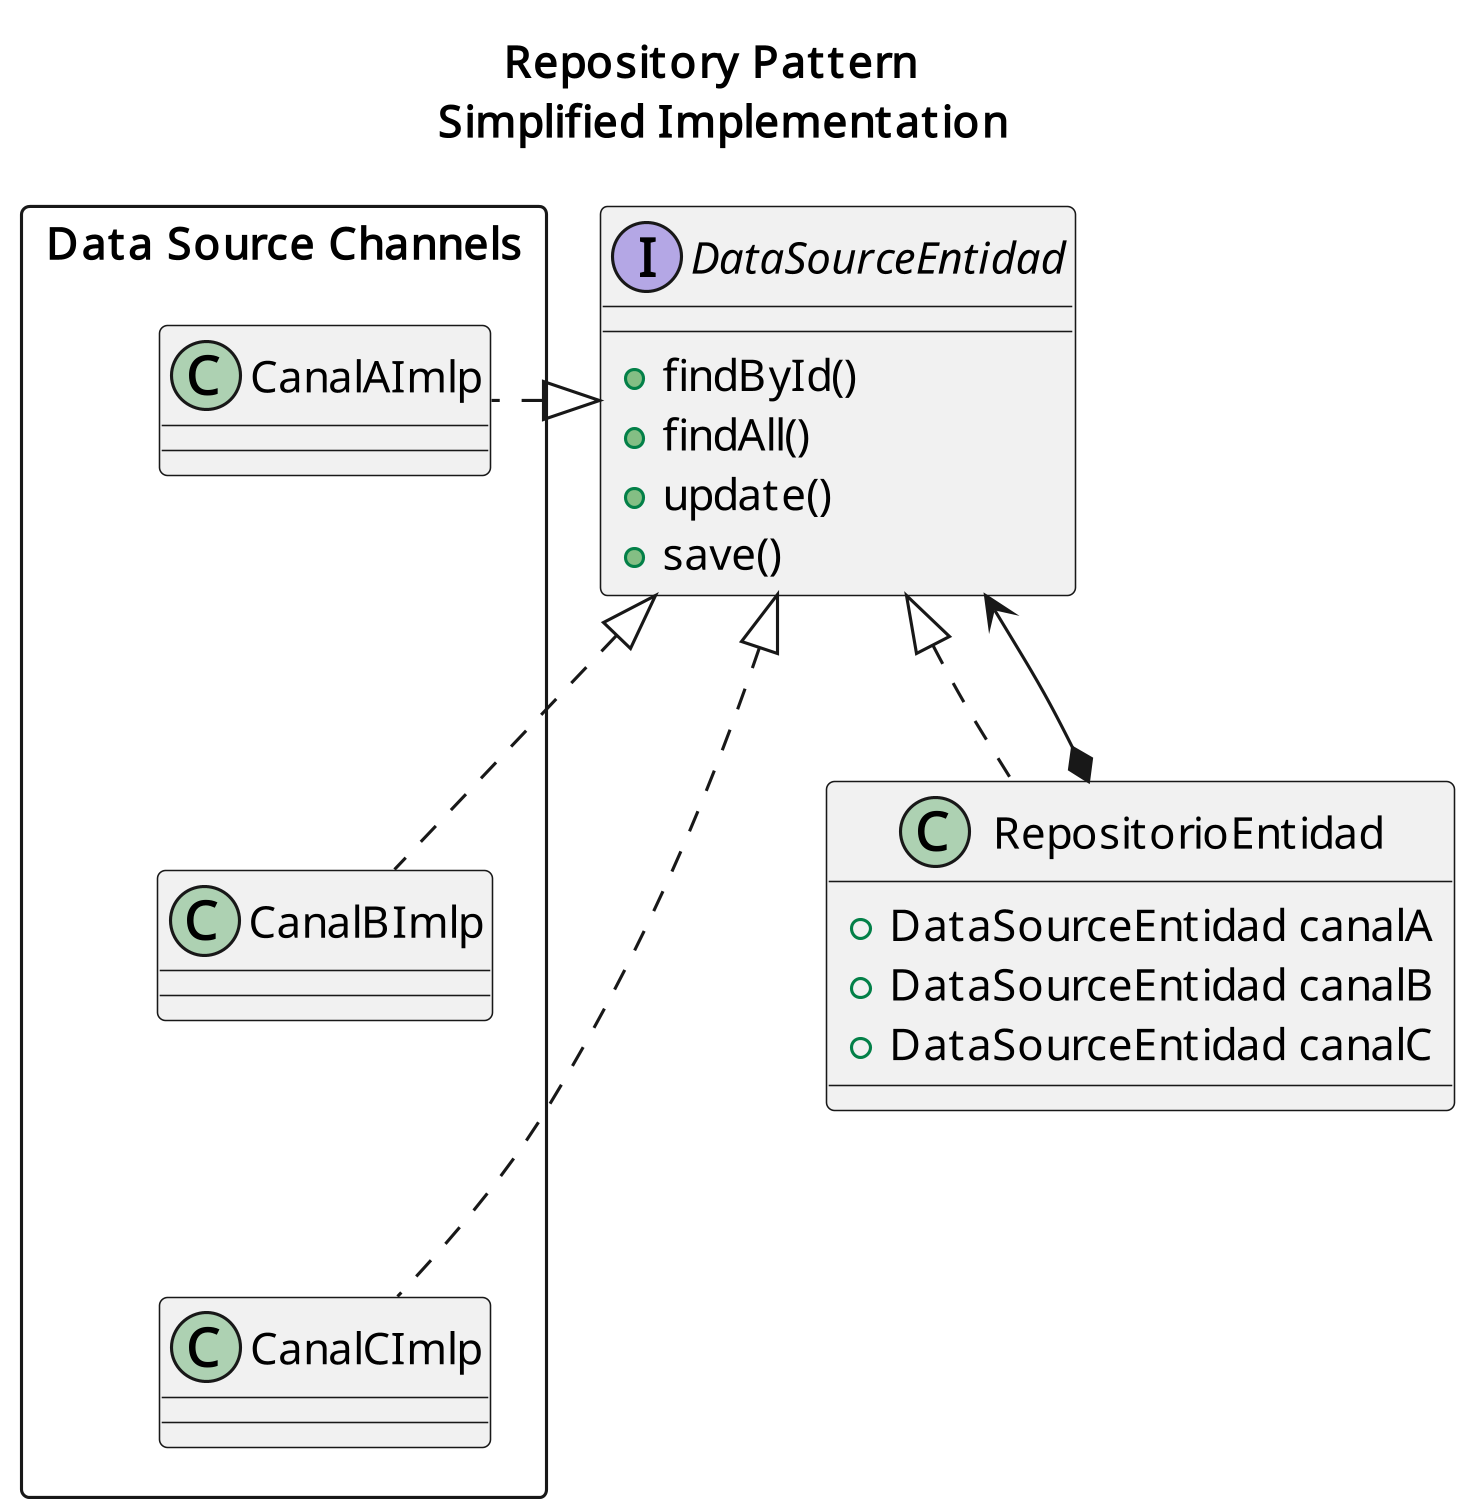
\includegraphics[width=0.5\textwidth]{Figures/design/CLASS_repository_reduced.png}
	\rule{35em}{1pt}
	\caption[Modified Repository Pattern Class Diagram]{Diagrama de clases del patrón Repository modificado.}
	\label{fig:uml_clases_modif_repository}
\end{figure}

Principalmente orientado a encapsular la manipulación, selección, priorización y mantenimiento de diversas fuentes u orígenes de datos, este diseño de repositorios modificado permite que el peticionario se comunique con una única interfaz para solicitar operaciones sobre datos permaneciendo agnóstico del origen  sobre el cual tendrán impacto. 
Implementar una política de caching local se convierte en una tarea sencilla de implementar y mantener.

\section{Programación Reactiva}
Se trata de un paradigma de programación cuya máxima sostiene que el código debe observar y reaccionar a estímulos internos y externos como eventos, interrupciones, resultados, etc. Estos estímulos por lo general se manifiestan como unidades de datos y tienen como característica principal su naturaleza asíncrona o de sucesión impredecible. Por lo que el código deberá observar de manera continua la ocurrencia de estos y reaccionar consecuentemente. En la jerga, la sucesión de estímulos de una misma fuente se denomina flujo.

Se definen tres entidades fundamentales para este paradigma: los \textbf{Estímulos}, sus \textbf{Emisores} y quienes los \textbf{Observan}. También se admite la concatenación de este trío de entidades lo que produce operadores que podrán ,a su vez, generar el mismo flujo o uno modificado.

En términos meramente lingüísticos al adaptar un lenguaje de programación procedural u orientado a objetos para que soporte este paradigma se le confieren atributos que originalmente eran propios de la programación funcional como lo son la composición de funciones y el tratamiento de datos como flujos o secuencias, lo que permite un abordaje más natural a problemas que implican manejo de eventos, concurrencia y asincronía.
Así mismo la programación reactiva promueve la inmutabilidad y la pureza funcional, especialmente en la manipulación de datos a través de operadores. Los cuales en los flujos reactivos suelen aplicar transformaciones inmutables a los datos, lo que garantiza que los originales no se modifiquen y que las operaciones sean consistentes y predecibles.

En términos arquitectónicos este paradigma implica la implementación del patrón \emph{Observer} para los objetos que observan los estímulos y el patrón \emph{Iterator} para los emisores. Será necesario también convertir a las funciones en entidades del lenguaje con estatus de  \emph{First Class Citizen} para admitir su composición de manera genérica.

Afortunadamente, y de la mano de el proyecto ReactiveX, estas adaptaciones para lenguajes no funcionales se ofrecen como librerías que implementan las tres entidades, una colección de operadores y el manejo de las primitivas de concurrencia. En particular para Java existe la librería RxJava que es la que utilizaré en el proyecto.



\section{Interfaz Módulo - Aplicación}
\label{section:interfaces}
\emph{El monitoreo y control de los módulos se realiza utilizando la aplicación móvil.}

Tanto el módulo como la aplicación son sistemas de software independientes que se ejecutan en dispositivos de arquitecturas distintas. Dado que, por requerimientos del producto, ambos sistemas deben interactuar entre si, es necesario definir las tecnologías, protocolos y definiciones que faciliten la comunicación.

Para la configuración inicial el módulo genera un Access Point Wi-Fi, el teléfono android se conectará a éste generando una LAN IPv4 con solo estos dos dispositivos en conexión punto-a-punto. Utilizando esta red la aplicación enviará las credenciales del router WiFi para su operación regular.

La operación regular del producto requiere que el módulo electrónico y el teléfono con la aplicación estén conectados al mismo router Wi-Fi. De esta manera ambos dispositivos pertenecen a la misma LAN IPv4. El módulo anunciará su presencia en la red para que la aplicación pueda encontrarlo y registre su dirección IP.

Ya sea para la configuración inicial o la operación regular el intercambio de mensajes se realiza utilizando el protocolo HTTP.

\begin{figure}[htbp]
	\centering
	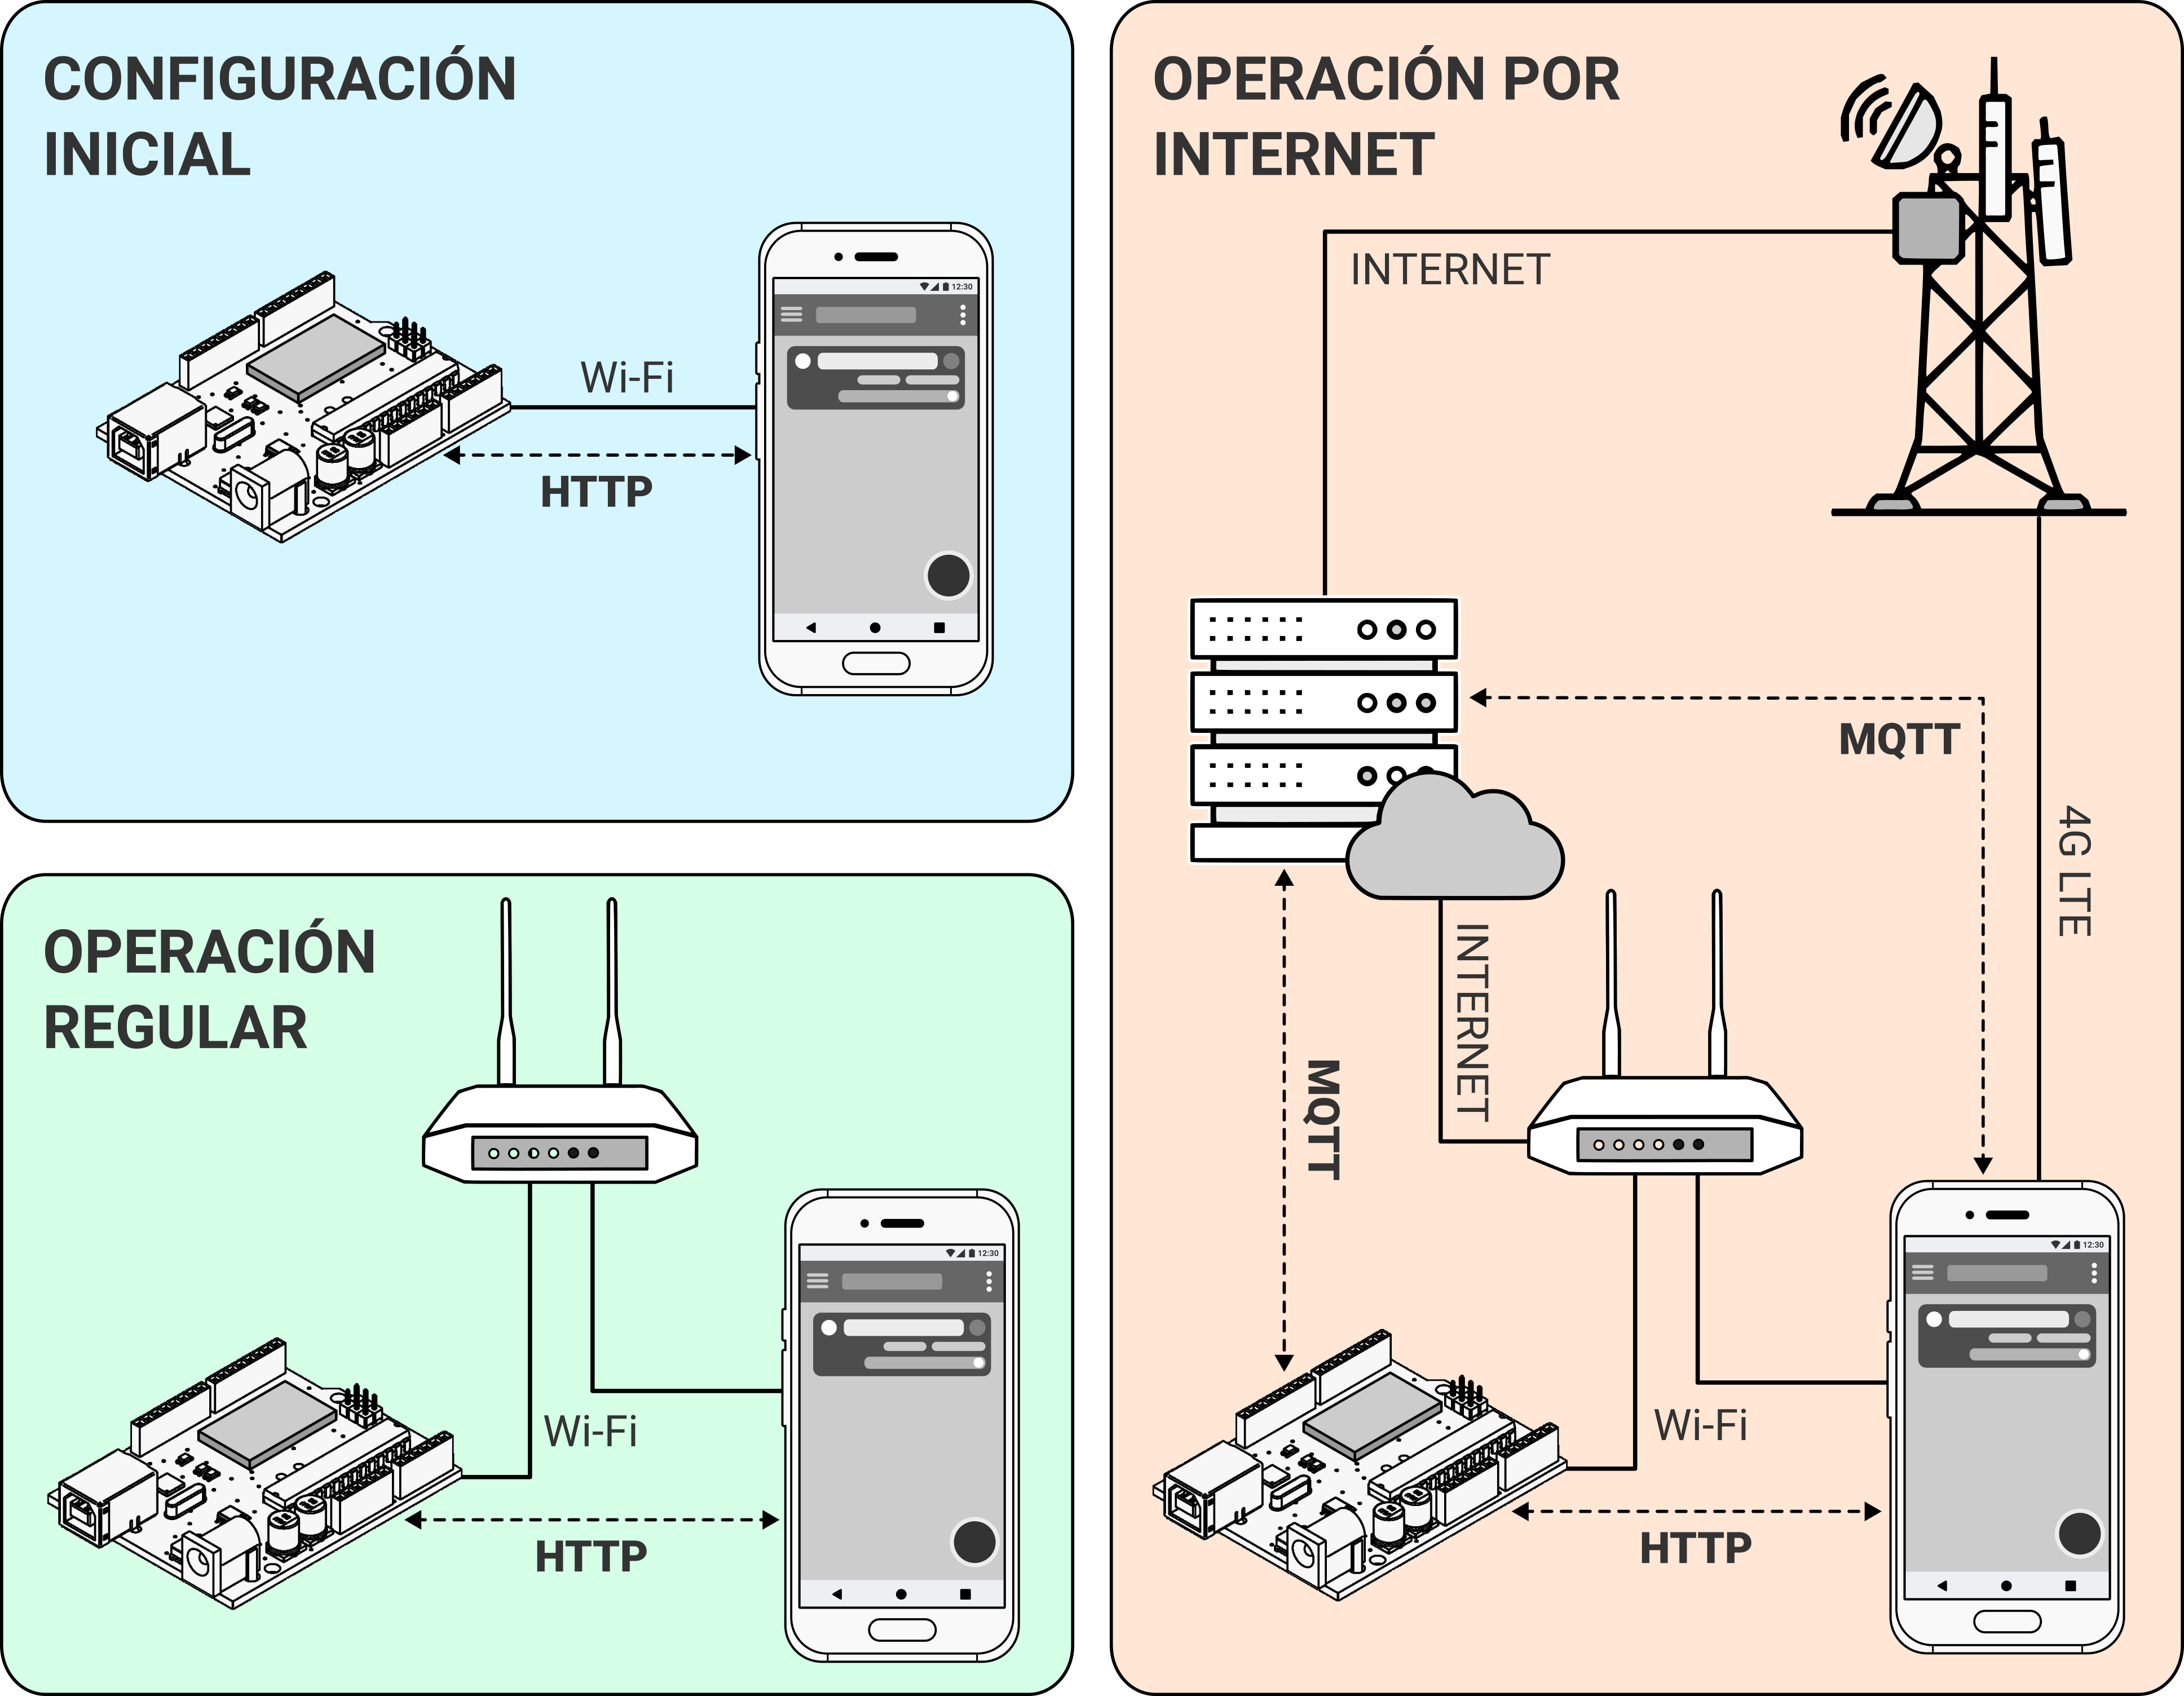
\includegraphics[width=0.9\textwidth]{Figures/design/conect.png}
	\rule{35em}{1pt}
	\caption[Esquema conexión Modulo-App]{Diagrama de comunicación entre módulo y aplicación.}
	\label{fig:comunic_mod_app}
\end{figure}

En una segunda etapa se extenderá el modo de comunicación entre el módulo y la aplicación móvil a través de internet empleando el protocolo MQTT. En la figura ~\ref{fig:comunic_mod_app} se puede observar una representación gráfica de los modos de operación soportados por el producto.

\subsection{Protocolos de Comunicación}
\subsubsection{MDNS DNS-SD}
\emph{La aplicación móvil podrá descubrir todos los módulos disponibles en la LAN.}

Para conseguir esto se optó por utilizar un enfoque Zeroconf que emplee DNS-SD y mDNS para resolver los hostnames de los módulos compatibles y sus direcciones IP. Incluso en la literatura existe una confusión entre estos términos por lo que será debidamente aclarada antes de continuar.

\begin{figure}[htbp]
	\centering
	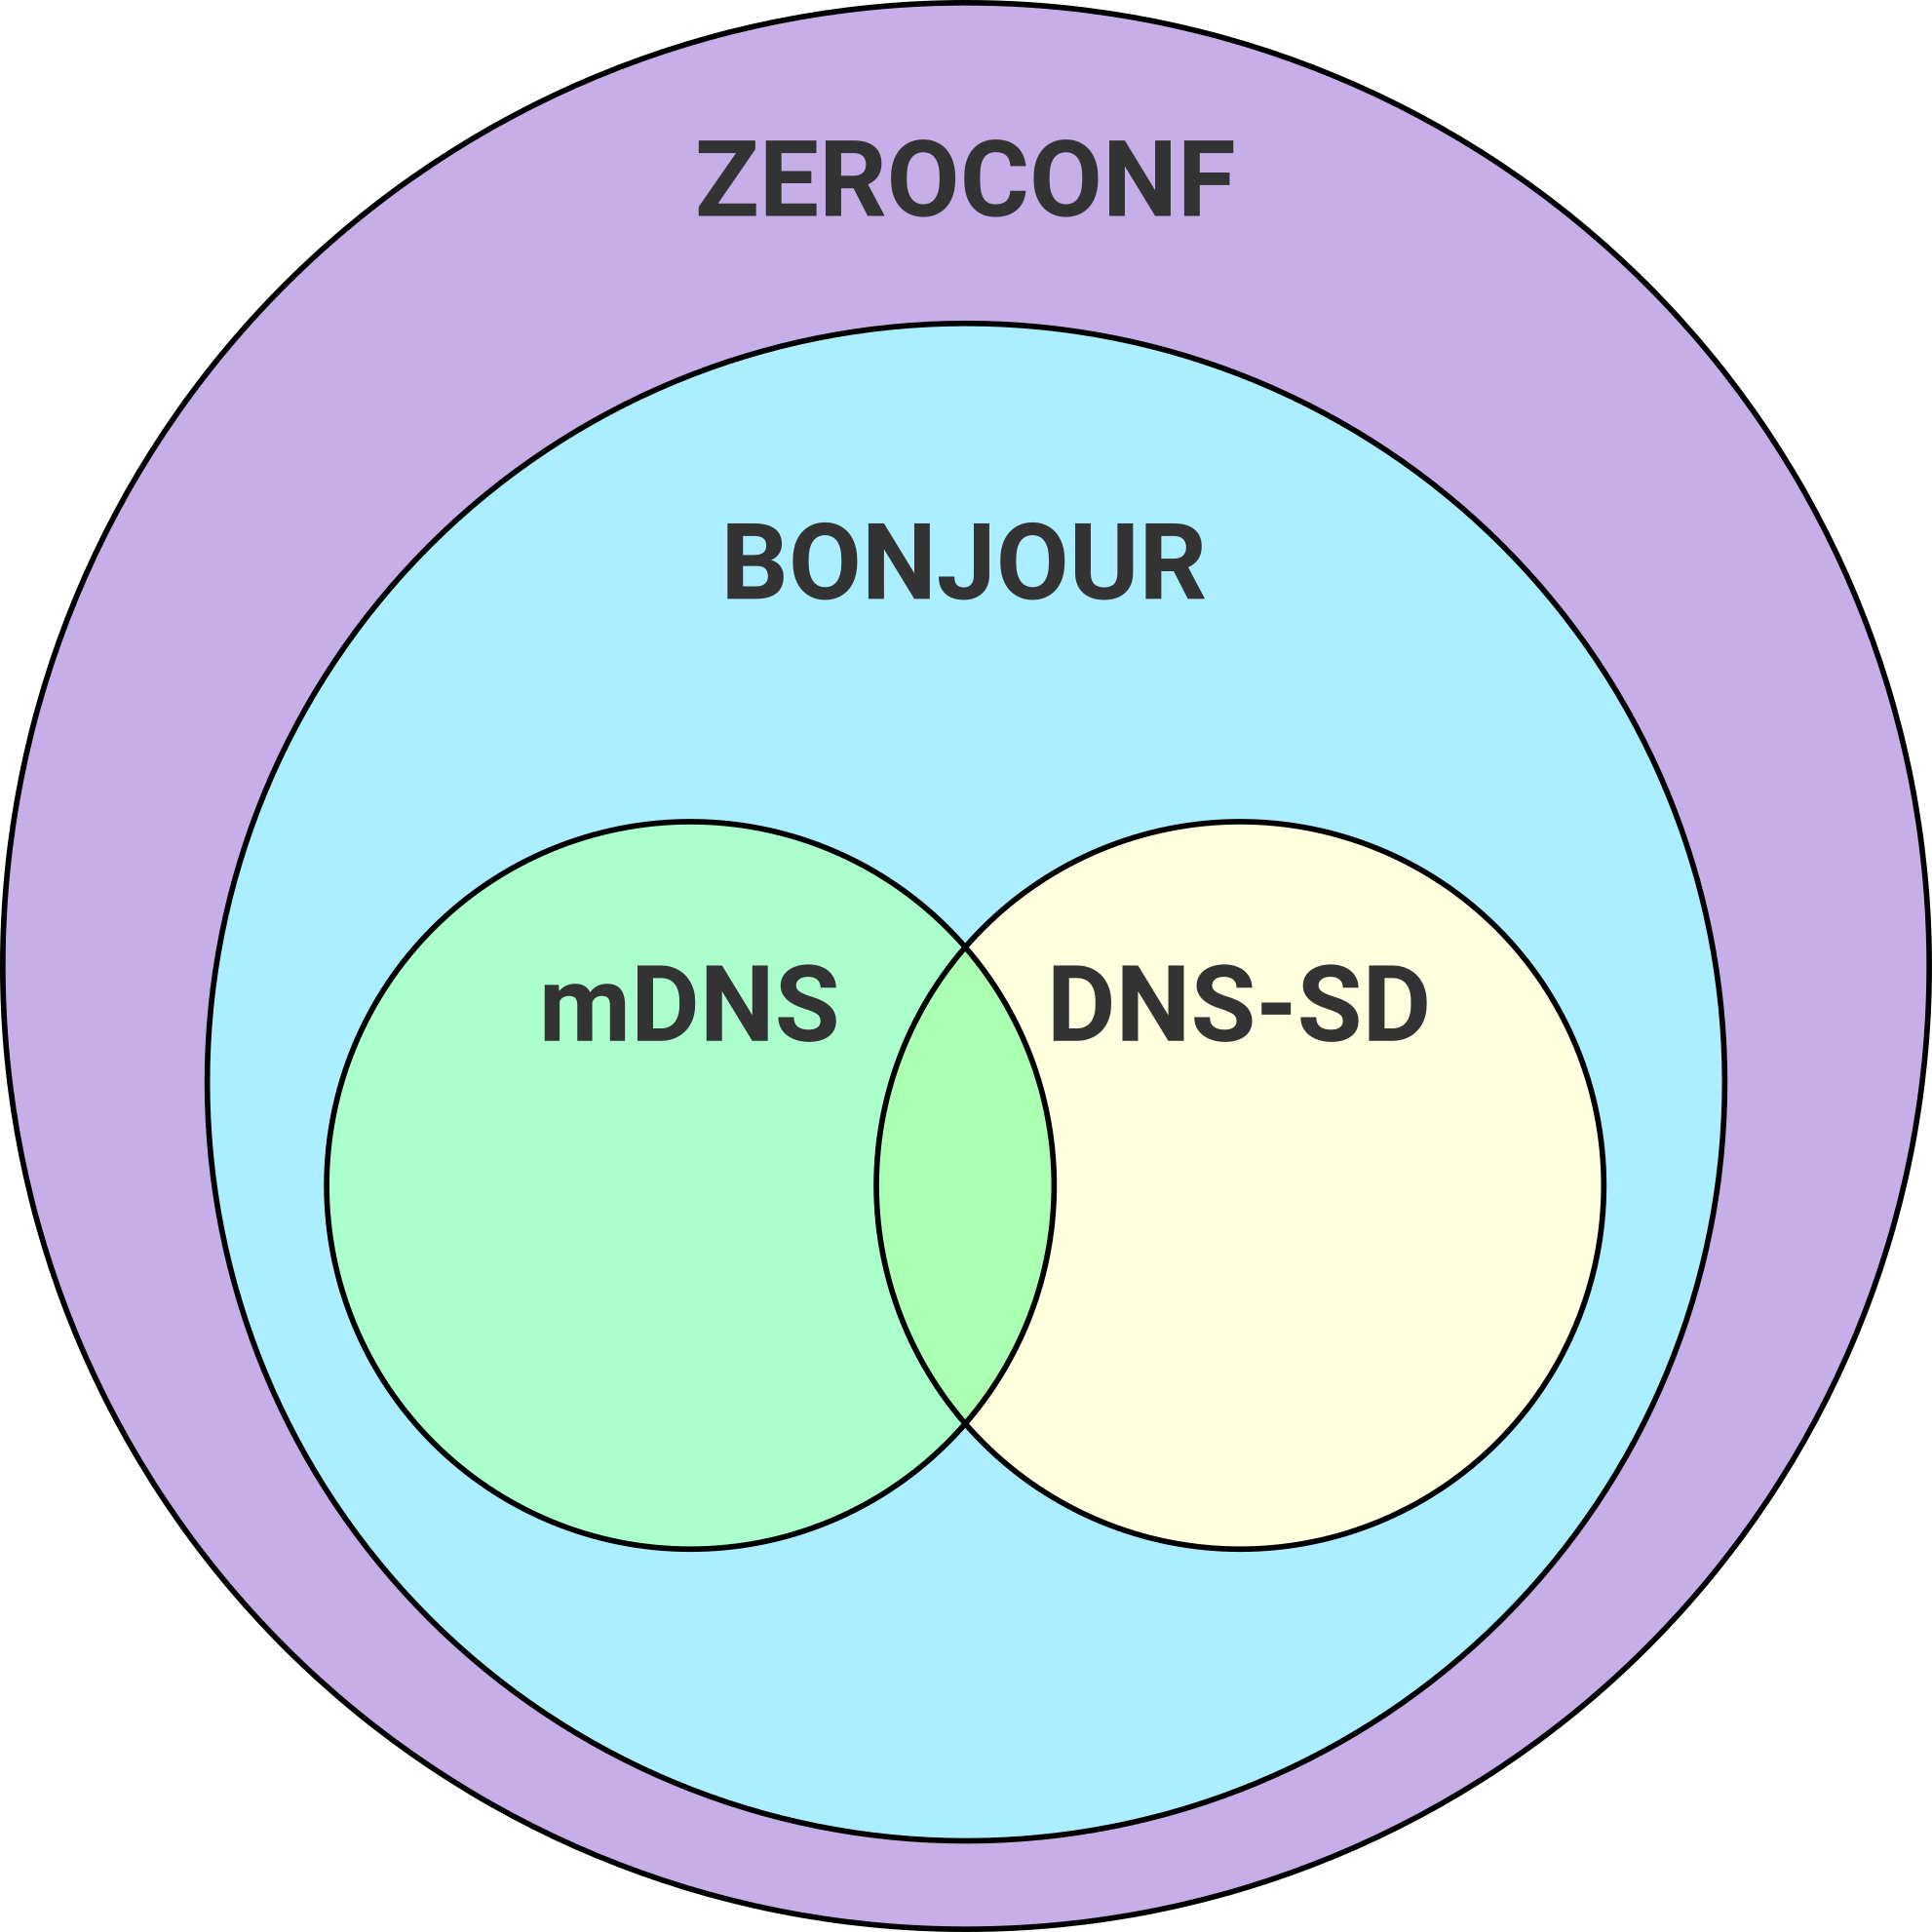
\includegraphics[width=0.4\textwidth]{Figures/design/zeroconf_venn.png}
	\rule{35em}{1pt}
	\caption[Desambiguación Zeroconf]{Diagrama de Venn que ilustra la relación entre los términos.}
	\label{fig:zeroconf_venn}
\end{figure}

\textbf{Zeroconf} (Zero Configuration Networking) no es un estándar sino un termino acuñado en la década de 1990 para denotar a la colección de protocolos y tecnologías que habilitan la configuración automática de redes y el descubrimiento de servicios en redes locales.

\textbf{mDNS} es un protocolo de capa de aplicación (RFC 6762) y se presenta como una extensión sobre \emph{DNS unicast} para la resolución de nombres en redes de área local. Este protocolo resuelve exclusivamente nombres de host que terminan con \texttt{.local} como dominio raíz. A diferencia de DNS la información de resolución se almacena localmente en cada dispositivo de la red y el intercambio de mensajes se realiza a una dirección multicast dónde cada dispositivo responde directamente a las consultas. 

\textbf{DNS-SD} es un estándar de capa de aplicación (RFC 6763) que permite a clientes DNS descubrir instancias nombradas de un servicio utilizando registros DNS (RR). Una instancia de servicio en DNS-SD se describe utilizando los siguientes RR: SRV, TXT, PTR y A/AAAA. 
\begin{itemize}
	\item PTR proporciona el mapeo entre tipos de servicio e instancias de servicio que lo proveen.
	\item SRV contiene información de la instancia de servicio, tipo de servicio (protocolo) peso, puerto y endpoint. Los parámetros de prioridad y peso dan preferencia cuando el mismo servicio es proporcionado por múltiples instancias. El parámetro endpoint respeta el formato de nombre de host.
	\item TXT contiene los metadatos del servicio en forma de pares [clave]:[valor]. El contenido exacto depende del protocolo utilizado.
	\item A/AAAA Resuelve una dirección IP a partir de un nombre de host.
\end{itemize}
En mDNS/DNS-SD, todos los RRs que describen una instancia de servicio se almacenan en el nodo que proporciona tal servicio. Un ejemplo de intercambio de mensajes mediante el cual se realiza el descubrimiento de un servicio se muestra en la figura ~\ref{fig:zeroconf_seq}.

\textbf{Bonjour} es una implementación zeroconf desarrollada por Apple. Emplea mDNS como protocolo de comunicación y DNS-SD para el descubrimiento y descripción de los servicios.

\begin{figure}[htbp]
	\centering
	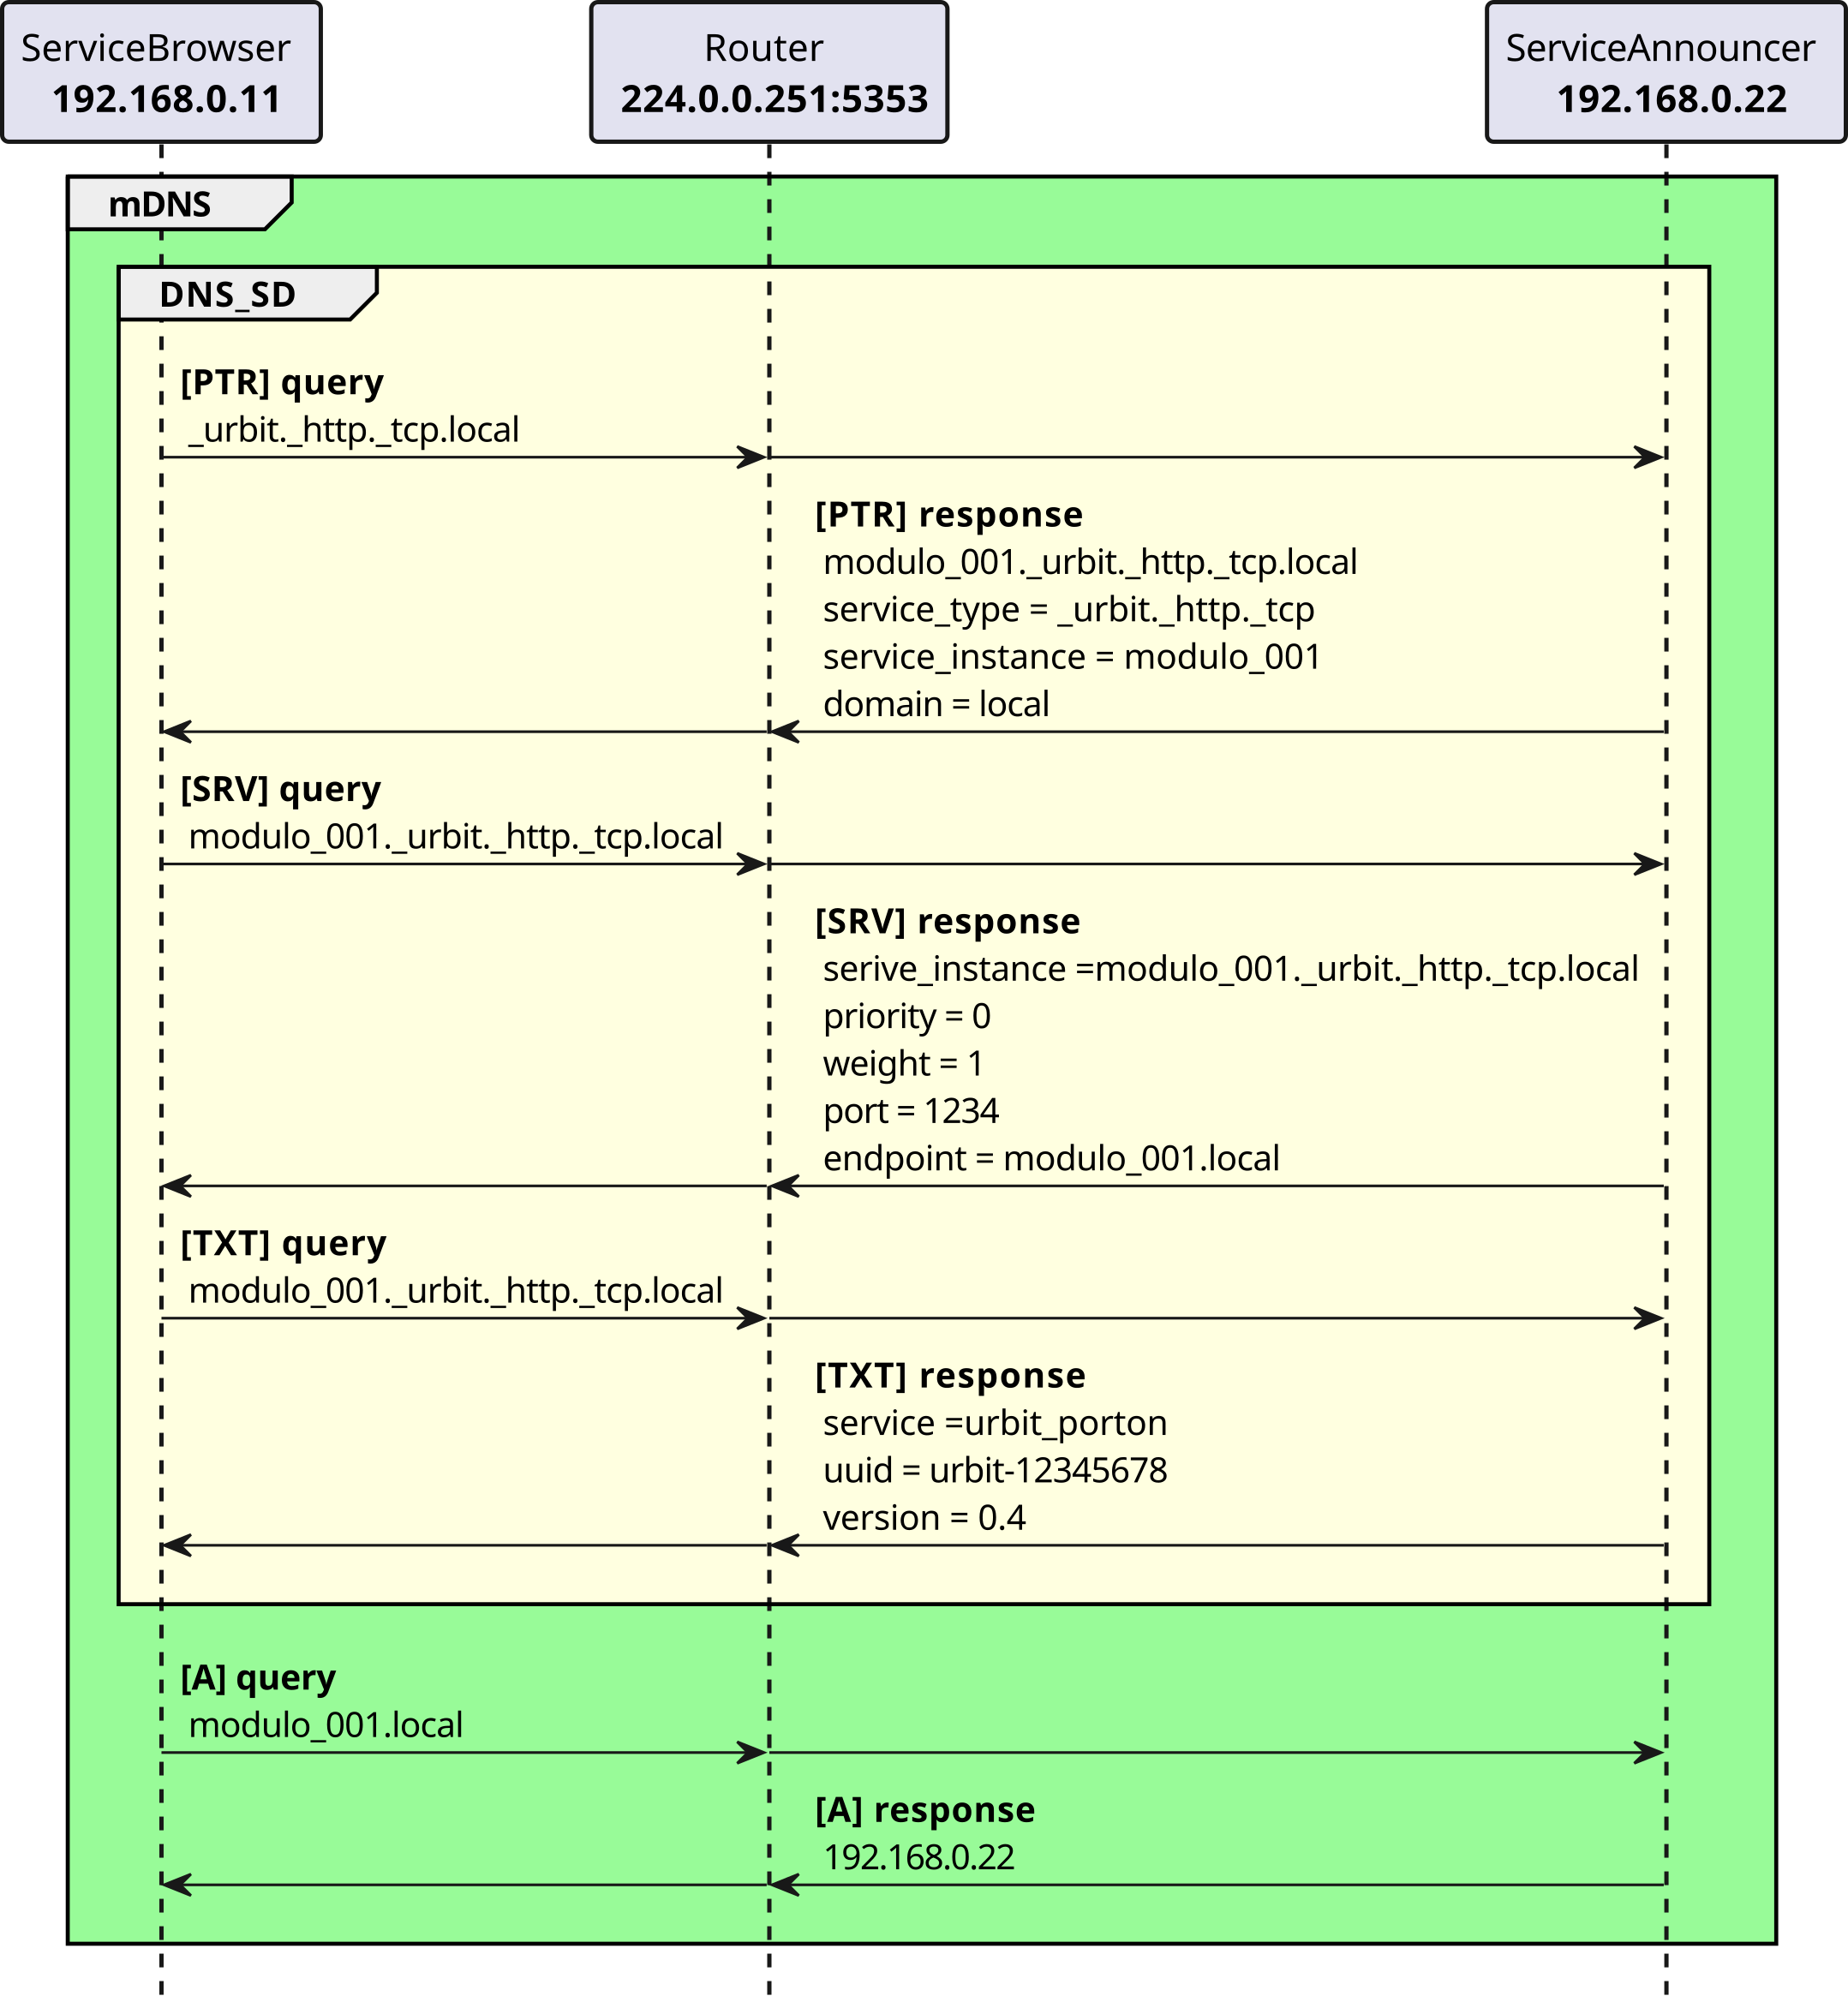
\includegraphics[width=0.8\textwidth]{Figures/design/SEQ_mdns_dnssd_ink.png}
	\rule{35em}{1pt}
	\caption[mDNS y DNS-SD]{Secuencia del descubrimiento de servicios.}
	\label{fig:zeroconf_seq}
\end{figure}

Android ofrece una API para el descubrimiento de dispositvos \emph{Network Service Discovery API} pero ésta no soporta la consulta de registros TXT. Google ofrece también la \emph{Google Nearby API} una librería de similares características pero que es de código cerrado y no proporciona el nivel de granularidad adecuado para este proyecto. Por estos motivos se optó por emplear la librería \emph{RxDNSSD} de andriydruk \cite{RxDNSSD} que hace de wrapper reactivo sobre la implementación oficial de Bonjour.

\subsubsection{HTTP y Digest Authentication}
\label{section:digest}
\emph{El módulo y la aplicación se comunican por defecto utilizando HTTP.}
 
El uso normal del producto implica la autenticación y la autorización de los usuarios por parte del módulo. Estas operaciones requieren el envío y la corroboración de las credenciales de usuario. 
El enfoque más básico \emph{Basic Authentication} realiza el intercambio de las credenciales en texto plano lo que implica un gran riesgo de seguridad.
Se evaluaron diversas alternativas para securitizar esta tarea y se optó por emplear \emph{Digest Authentication}.

\begin{figure}[htbp]
	\centering
	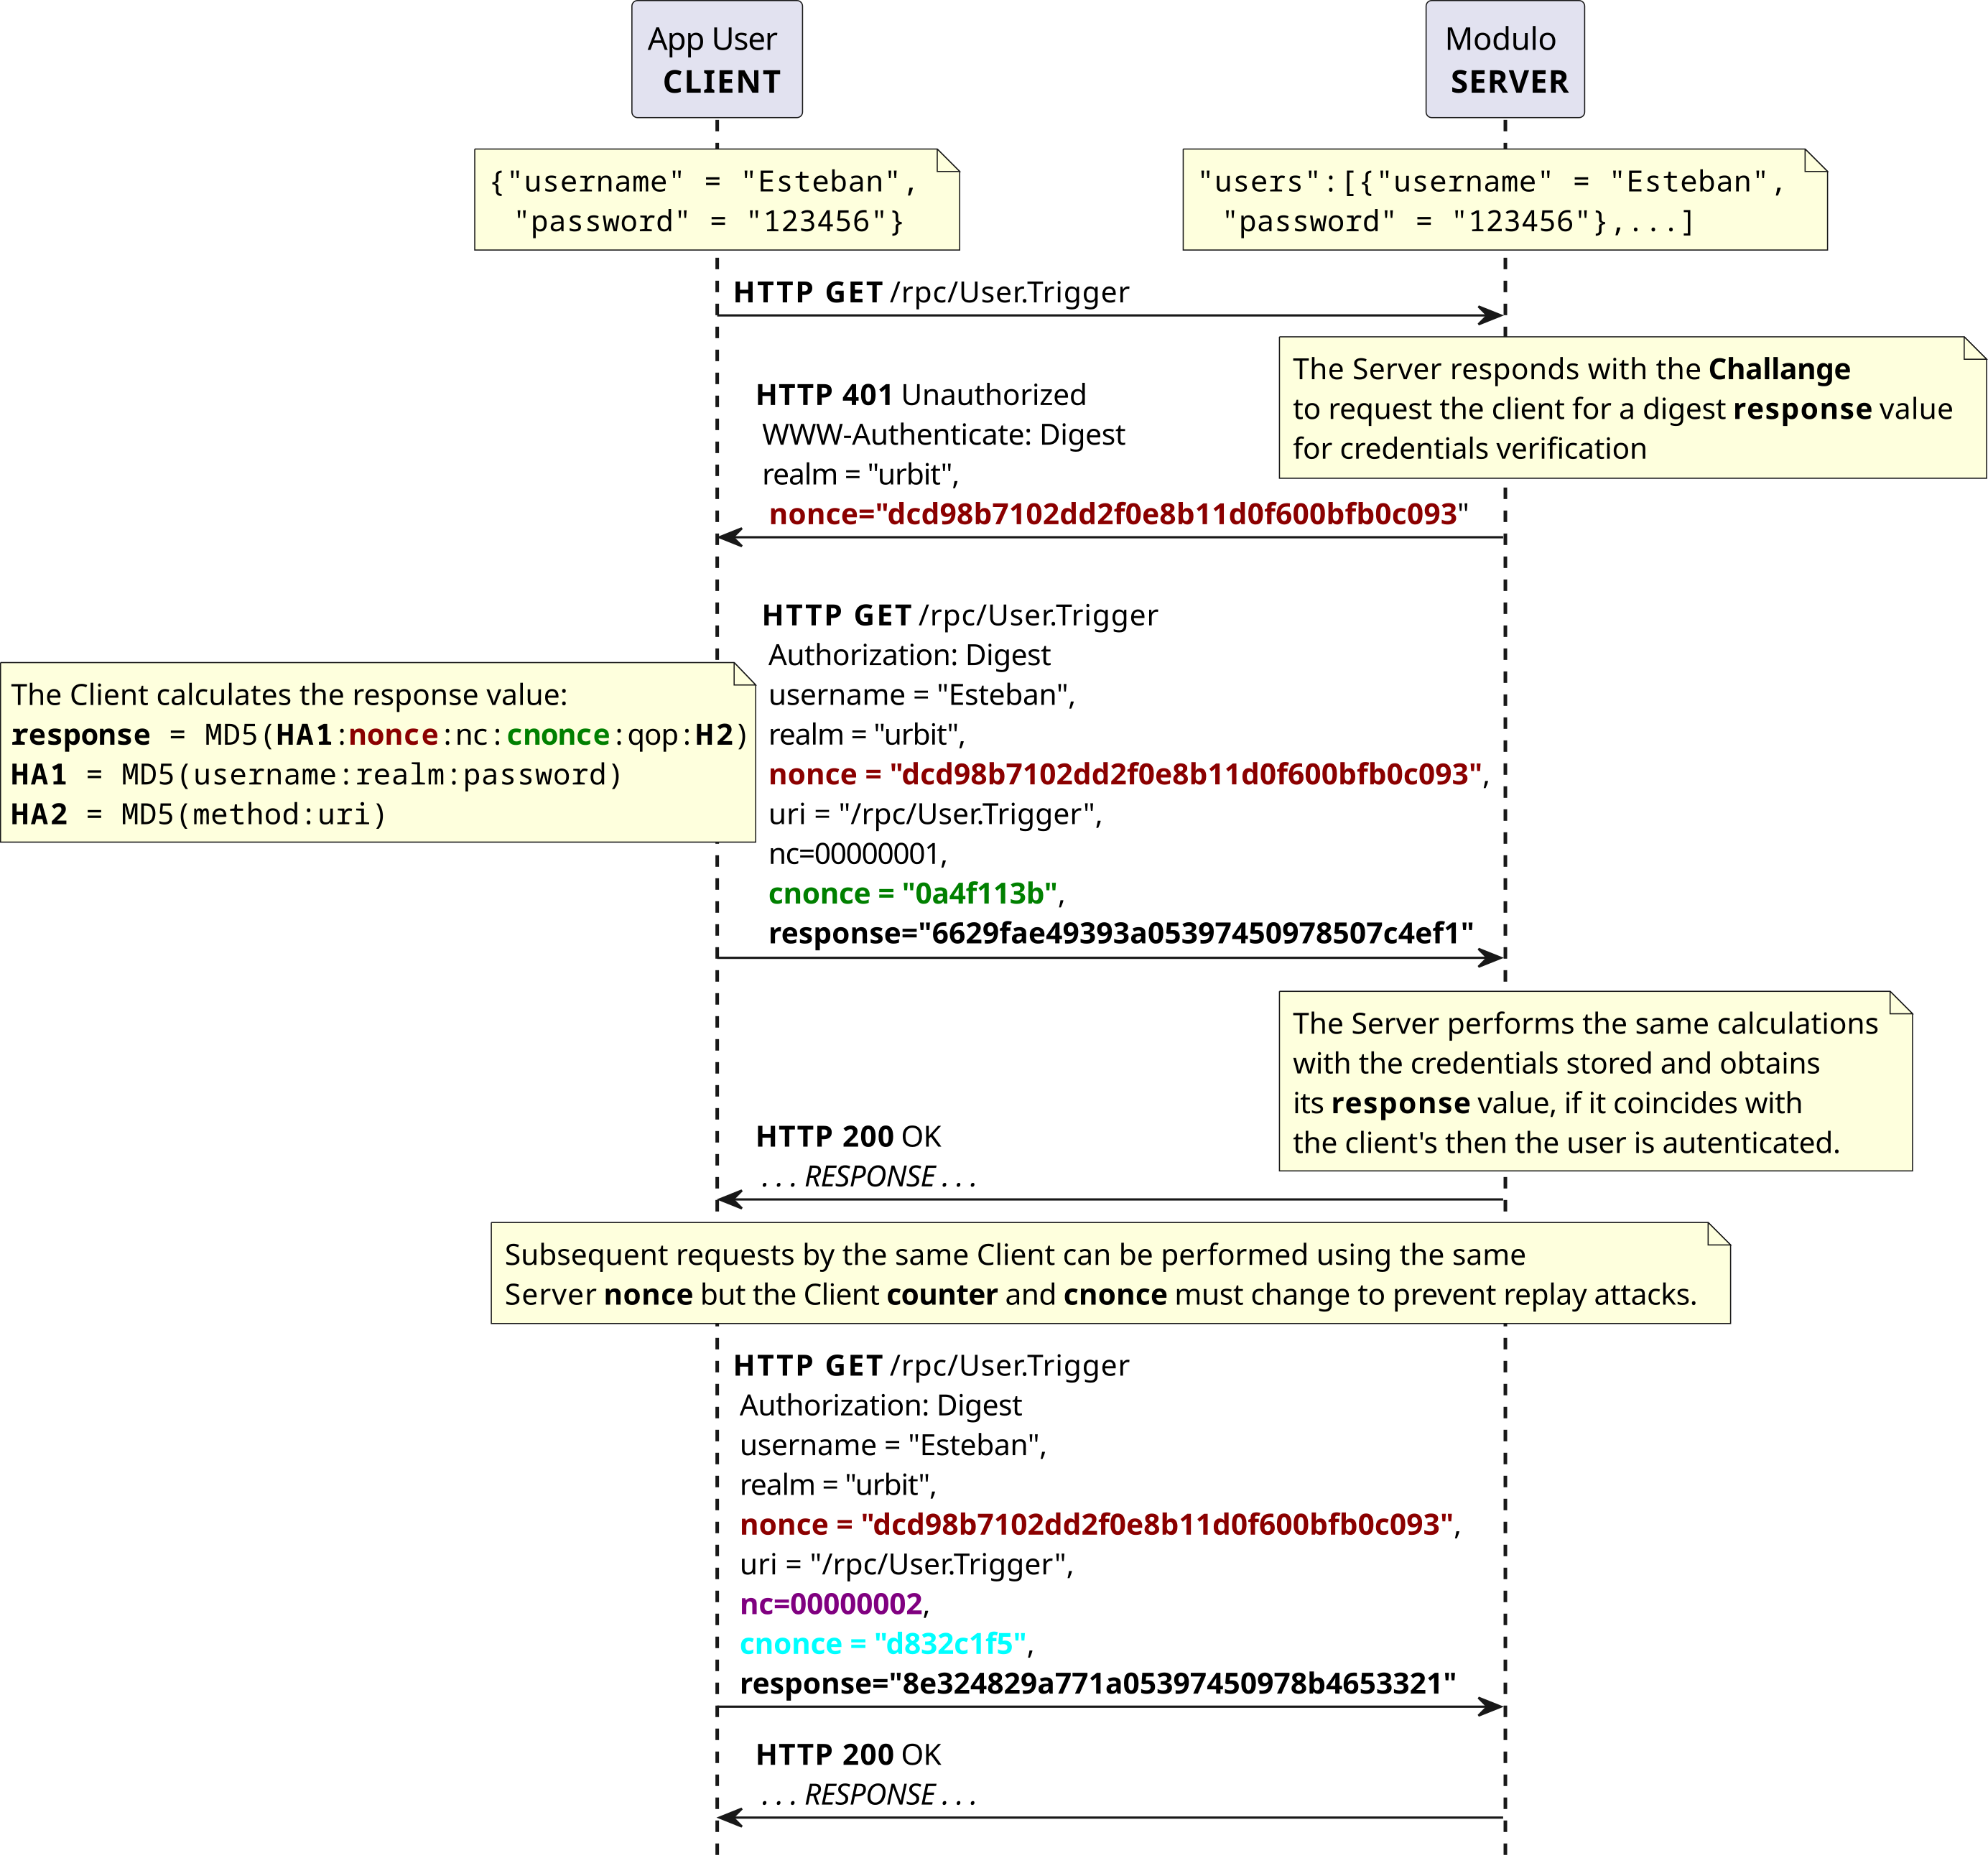
\includegraphics[width=\textwidth]{Figures/design/SEQ_digest_auth_ink.png}
	\rule{35em}{1pt}
	\caption[Secuencia HTTP Digest Authentication]{Secuencia de la autenticación utilizando Digest Authentication.}
	\label{fig:digest_auth_seq}
\end{figure}

\textbf{Digest Authentication} es un esquema de autenticación (RFC 2617) para comunicaciones HTTP cuyo propósito es proveer un método de autenticación de acceso que evite las fallas más serias de Basic Authentication.
Este esquema requiere la realización de un intercambio inicial entre el servidor y el cliente para verificar las credenciales de usuario. El procedimiento se describe a continuación, un ejemplo detallado se muestra en la figura ~\ref{fig:digest_auth_seq}.
\begin{enumerate}
	\item El cliente hace una solicitud con parámetros de autenticación incorrectos o ausentes.
	\item El Servidor responde con el challenge solicitando que el cliente calcule y envíe el valor  response.
	\item El cliente genera todos los argumentos necesarios, calcula el valor response y replica la solicitud original con estos datos adjuntos como HEADER.
	\item El Servidor hace el mismo cálculo y compara su resultado con el recibido del cliente. Si coinciden entonces se autentica al usuario y se procede con la consulta.
\end{enumerate}

Una vez autenticado, el cliente puede realizar nuevas solicitudes utilizando el mismo \textbf{nonce} del servidor para calcular el valor \textbf{response}. Sin embargo es necesario que el cliente actualice \textbf{cnonce} y el contador \textbf{nc} para prevenir ataques de tipo \emph{replay attack}. 

\subsubsection{MQTT}
\label{section:mqtt}
\emph{Uno de los atractivos del producto es la posibilidad de monitorear y accionar módulos de manera remota.}

Para que esto sea posible es necesario que tanto el módulo como la aplicación móvil tengan acceso a internet ~\ref{fig:comunic_mod_app}. Luego de discutir alternativas el equipo decidió que la comunicación por internet se realizará utilizando  MQTT.

MQTT es un protocolo de capa de aplicación (RFC 9431) diseñado para el intercambio de mensajes machine-to-machine (M2M) en redes de bajo ancho de banda y alta latencia. Este protocolo de comunicación se construye utilizando la arquitectura publish-suscribe mediante la que proporciona un servicio de colas de mensajes. Su implementación en los clientes es liviana por lo que se puede utilizar en sistemas embebidos de bajos recursos de hardware, razón por la cual es ideal para este proyecto.

\begin{figure}[htbp]
	\centering
	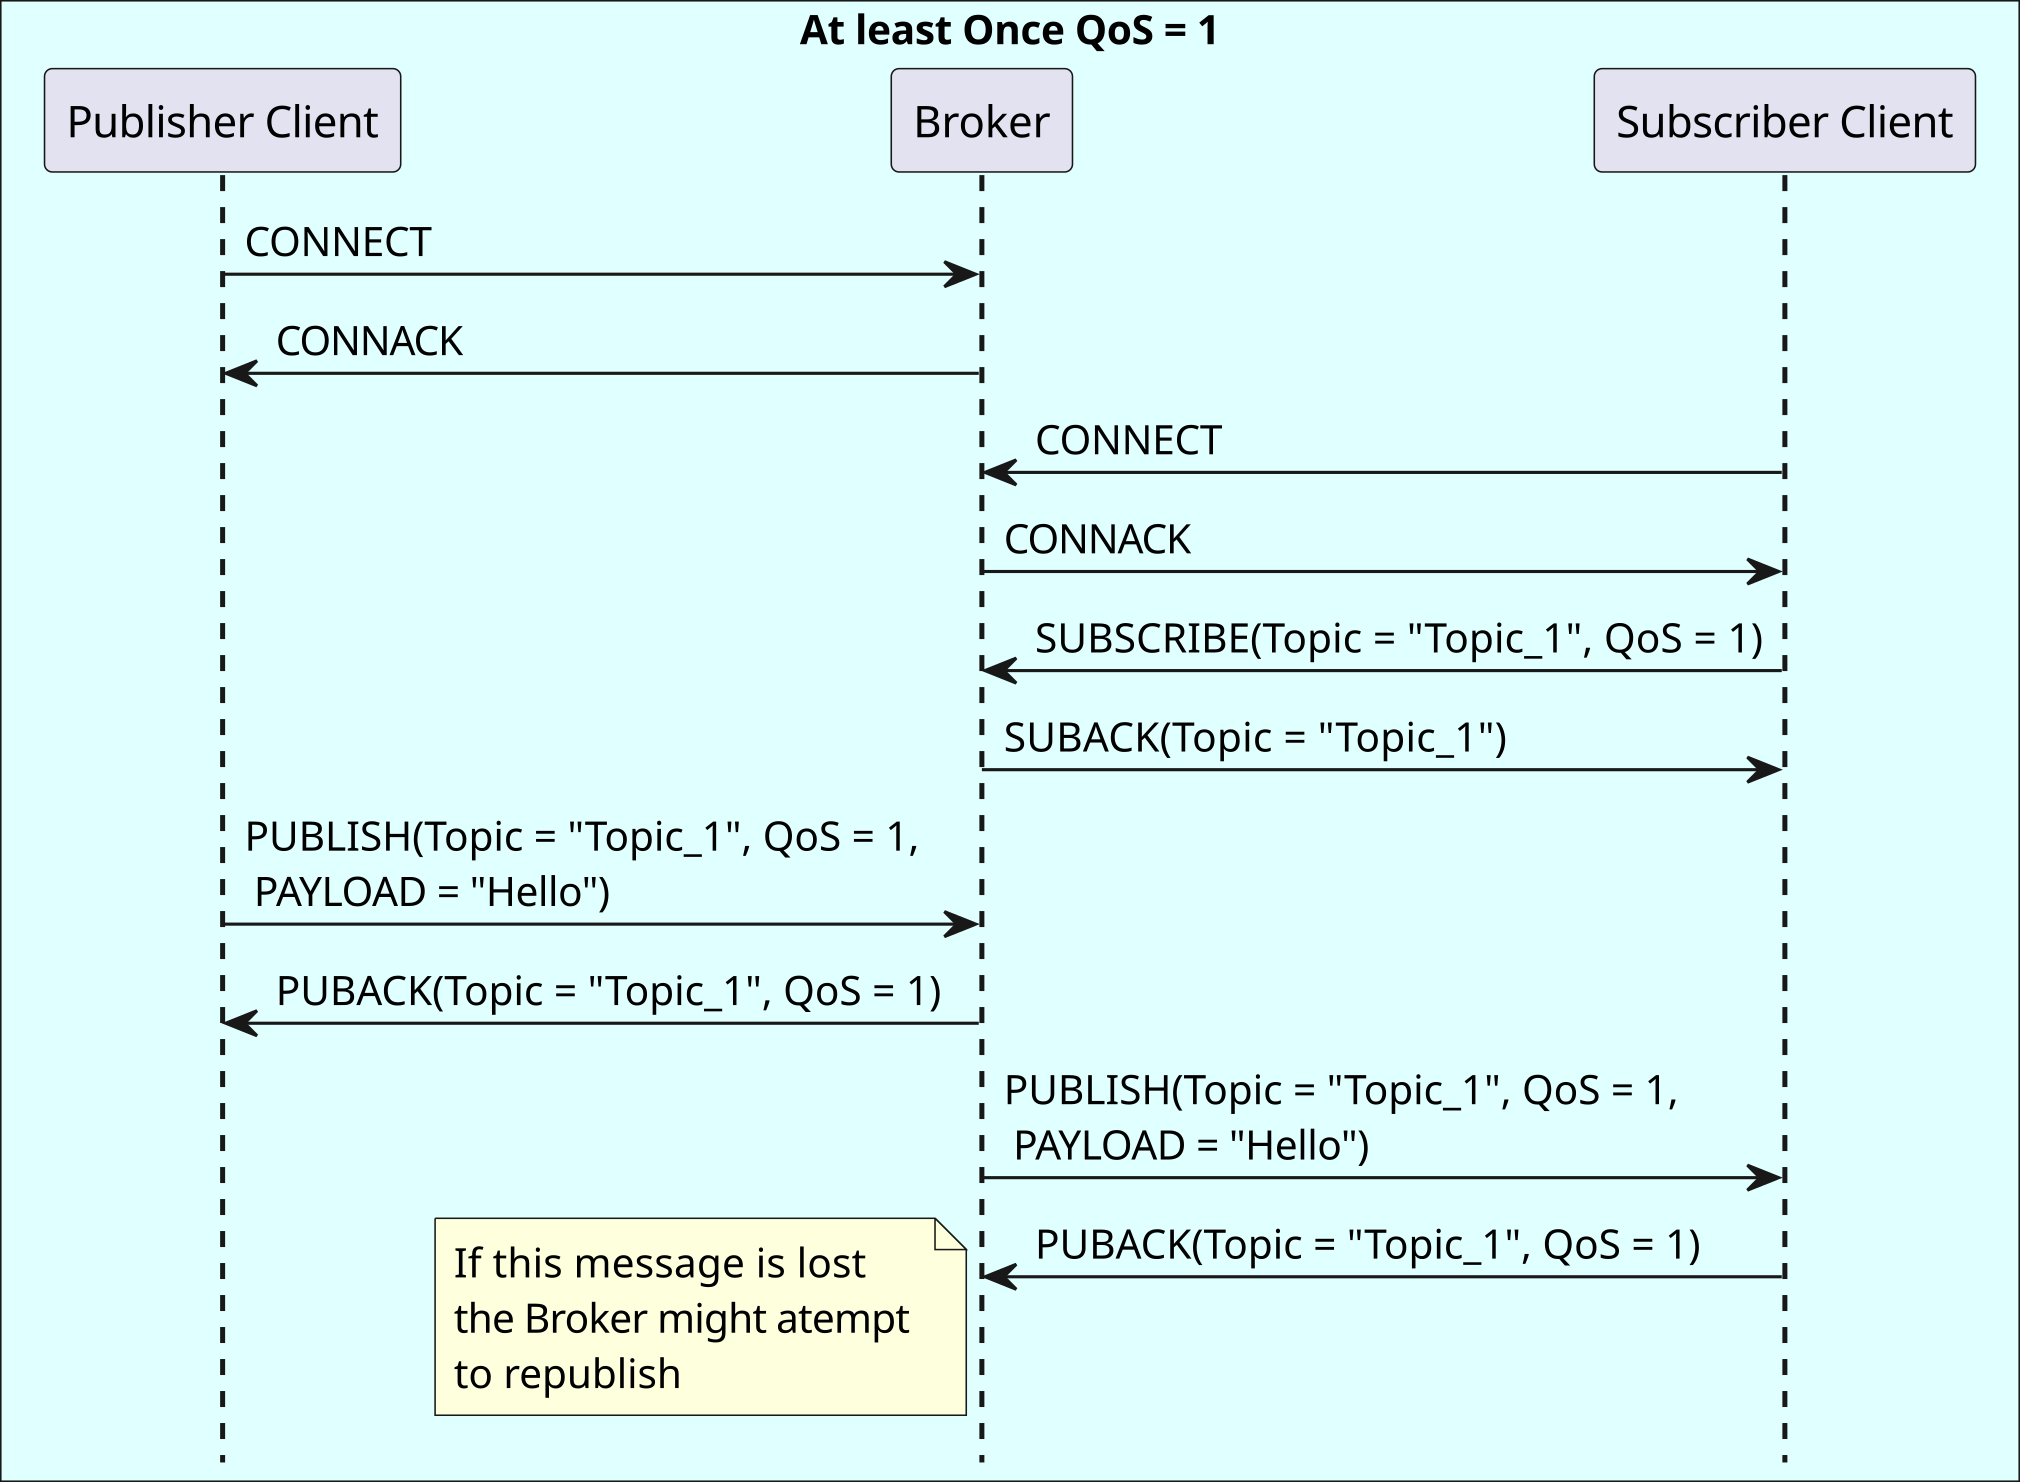
\includegraphics[width=0.8\textwidth]{Figures/design/SEQ_mqtt_ink.png}
	\rule{35em}{1pt}
	\caption[Secuencia MQTT QoS=1]{Secuencia del envío de mensajes par $QoS = 1$.}
	\label{fig:mqtt_seq}
\end{figure}

Para su funcionamiento es fundamental el rol de un agente que se denomina Broker. Este hace de intermediario entre los clientes conectados que envían mensajes y quienes los reciben.
Los clientes pueden suscribirse a múltiples Tópicos para recibir los mensajes que se publican en cada uno de ellos. Así mismo los clientes pueden publicar mensajes en Tópicos existentes o crear nuevos.
En consecuencia el Broker debe mantener un registro de los clientes, tópicos y suscripciones. Un ejemplo de envío de mensajes se muestra en la figura ~\ref{fig:mqtt_seq}.

Todos los clientes envían de forma periódica el mensaje KEEP\_ALIVE al Broker con el propósito de mantener actualizadas sus direcciones IP y el estado de las sesiones.

Haciendo uso de estas características el protocolo consigue establecer un canal de comunicación continuo y persistente entre los clientes del servicio.

Los pormenores de la adaptación de este protocolo a los requerimientos del proyecto se detallaran más adelante.


\subsection{RPC API}
\label{section:rpc}
Como se expuso al inicio de la sección ~\ref{section:interfaces} el módulo y la aplicación deben interactuar entre sí empleando diversos protocolos de comunicación.
Si bien se detallaron los medios y los procedimientos, aún falta definir el formato de los mensajes que intercambiarán para garantizar la ejecución de las funcionalidades.

Con este propósito se analizaron diversas alternativas utilizadas en la industria y se optó por especificar una API RPC.

\textbf{RPC} (Remote Procedure Call) o ejecución de procedimientos remotos es un protocolo de mensajes (RFC 1057, 5531) que permite a un sistema cliente ejecutar funciones en otro sistema servidor de manera transparente. 
\emph{El cliente llama al procedimiento como si fuera local y la implementación RPC subyacente se encarga de los detalles de comunicación.}

\begin{figure}[htbp]
	\centering
	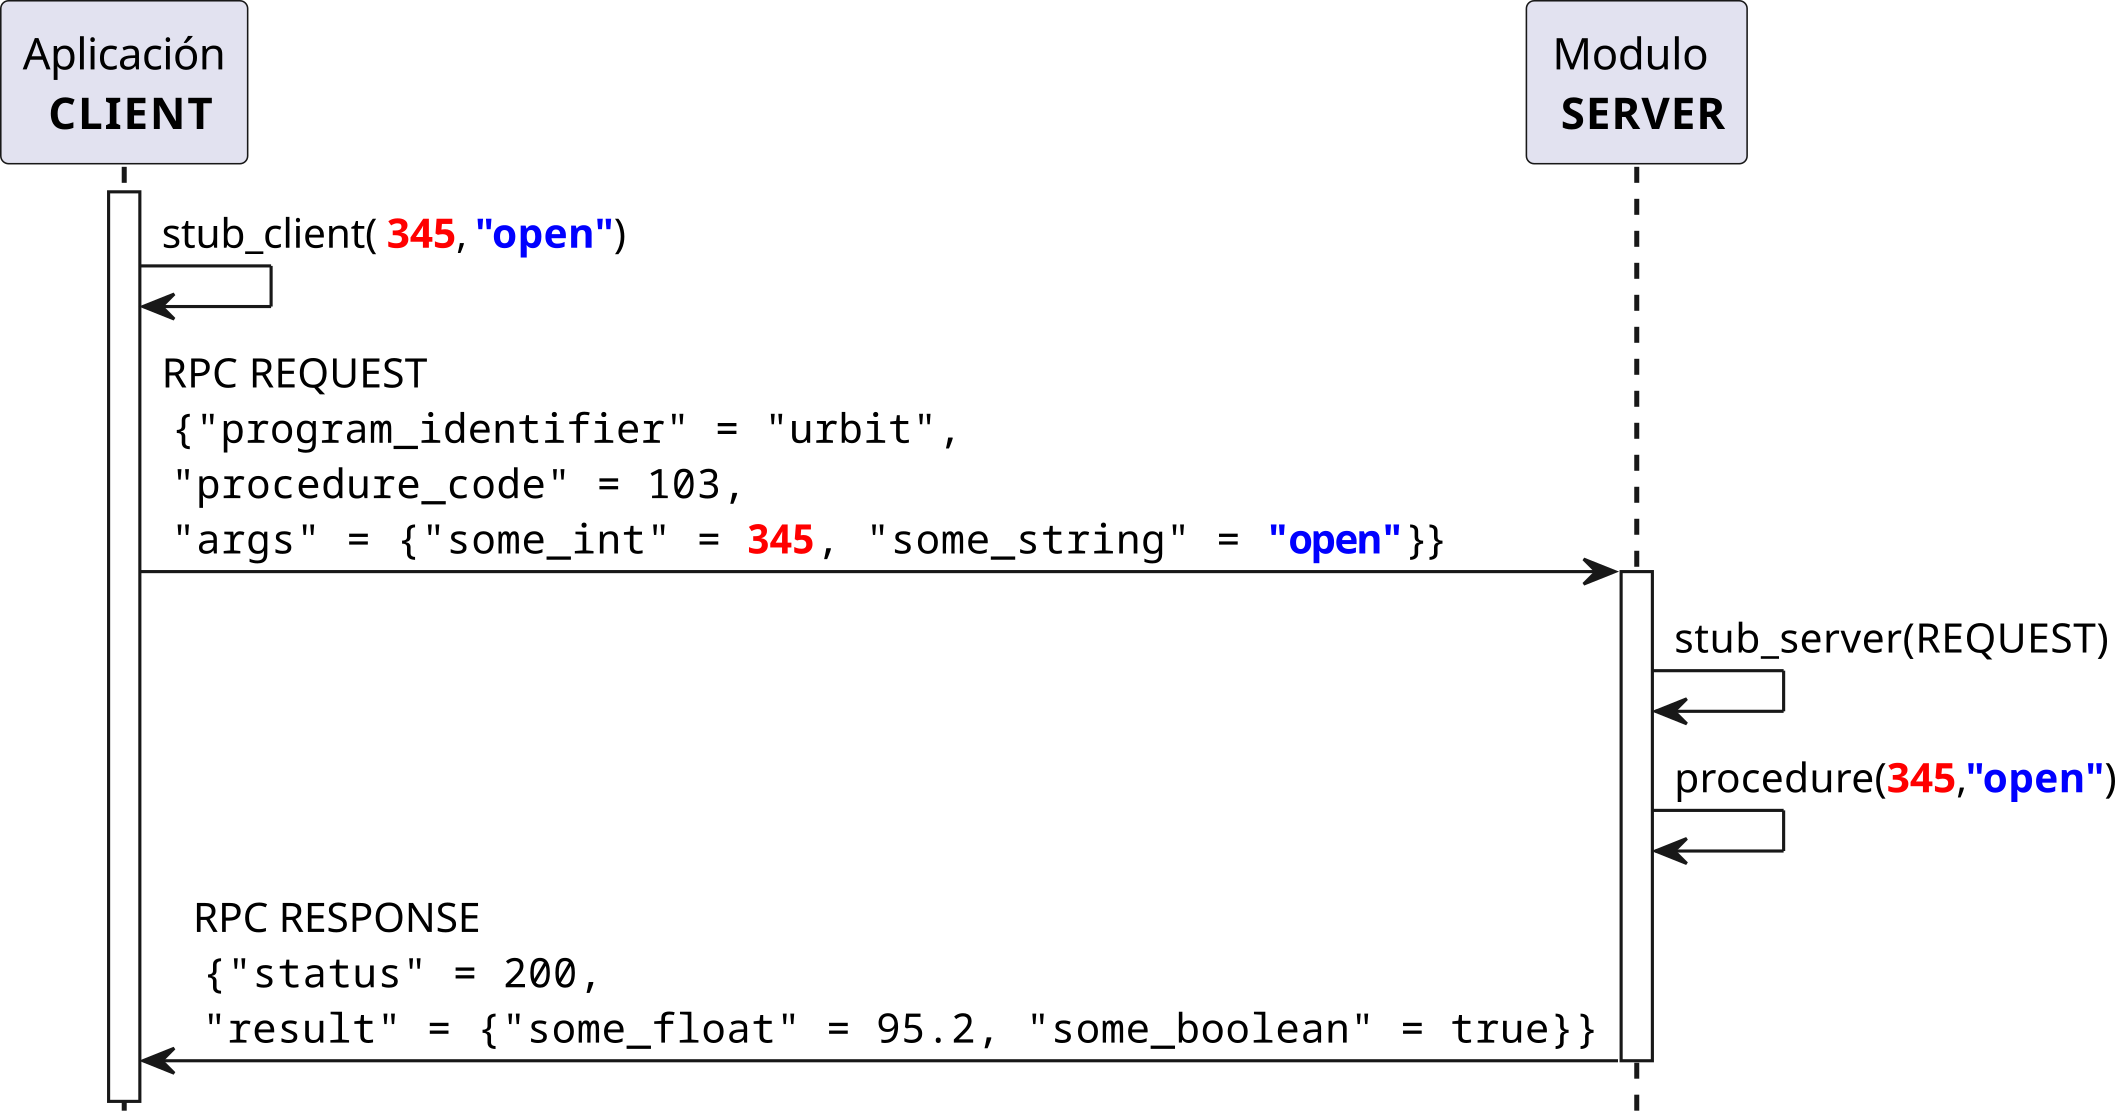
\includegraphics[width=0.8\textwidth]{Figures/design/SEQ_rpc_ink.png}
	\rule{35em}{1pt}
	\caption[Secuencia RPC]{Secuencia de ejecución de un procedimiento remoto.}
	\label{fig:seq_rpc}
\end{figure}

El protocolo implementa el patrón Request-Response que se compone de ``stubs'' o ``pasamanos'' de los procedimientos tanto en el cliente como en el servidor. Estos stubs son funciones que no ejecutan la lógica del procedimiento sino que se encargan de: construir estructuras de datos para solicitudes y respuestas, convertir estos objetos de memoria en otros con formatos de red, y los pormenores de su transmisión.


Elementos de una Solicitud (Request):
\begin{itemize}
	\item Identificador del programa
	\item Número del procedimiento
	\item Argumentos
\end{itemize}

Elementos de una Respuesta (Response):
\begin{itemize}
	\item Resultado o valore de retorno.
	\item Información de estado (Ejecución Exitosa, Error).
\end{itemize}

Por legibilidad y estandarización, solicitudes y respuestas tendrán formato JSON. En la figura ~\ref{fig:seq_rpc} se muestra un ejemplo de RPC.

\begin{multicols}{3} % Change 3 to desired number of columns
	
	% Your content for column 1
	El formato definitivo para Solicitudes:
	\begin{lstlisting}
{
  "id": 103,
  "method": "method_name",
  "params":{
    "un_parametro": ...,
    "otro_parametro": ...,
    ...
  }
}
	\end{lstlisting}
	
	\columnbreak % Insert a column break between columns
	
	% Your content for column 2
	El formato definitivo para Respuestas exitosas:
	\begin{lstlisting}
{
  "id": 103,
  "result":{
    "un_resultado": ...,
    "otro_resultado": ...,
    ...
  }
}
	
	\end{lstlisting}
	
	\columnbreak % Insert a column break between columns
	
	% Your content for column 3
	El formato definitivo para Respuestas con error:
	\begin{lstlisting}
{
  "id": 103,
  "error":{
    "code": 404,
    "message": "... no existe",
    ...
  }
}
	
	\end{lstlisting}
	
\end{multicols}
En una de las labores más tediosas del diseño se revisaron los casos de uso y a partir de ellos se definieron 17 procedimientos que la aplicación podrá utilizar para ejecutar en un módulo. La especificación completa se puede consultar en la tabla ~\ref{tab:rpc_api}.
La invocación de los procedimientos se realizará enviando consultas HTTP siempre utilizando el método POST.

\begin{sidewaystable}[!htbp] 
	\scriptsize
	\rowcolors*{1}{black!10}{}
	\begin{tabularx}{\columnwidth}{|c|>{\bfseries\ttfamily}l|>{\raggedright\arraybackslash}X|>{\ttfamily}X|>{\ttfamily}X|>{\tiny\ttfamily}X|}
		\hline
		\multicolumn{1}{|>{\bfseries}c|}{Código} & \multicolumn{1}{>{\bfseries}c|}{Protocolo} & \multicolumn{1}{>{\bfseries}c|}{Descripción}  & \multicolumn{1}{>{\bfseries}c|}{Argumentos} & \multicolumn{1}{>{\bfseries}c|}{Respuesta} & \multicolumn{1}{>{\bfseries}X|}{Errores
			\newline \tiny\texttt{401 Unauthorized  \newline
				403 Forbidden \newline \{``code'':int, ``message'':string\}}{}  } \\ \hline
		
		100  & Admin.FactoryReset   & Elimina las configuraciones y los usuarios registrados. & \{\}    & 
		\{"message":string\} &  \\  \hline
		
		101  & Admin.SetWiFiAP      &  Conecta el módulo a un Access Point WiFi.     &   \{"ssid": "string","password"": "string"\}      &  \{"message":string\}      &    	
		400 Bad Request \newline
		[ssid and password required] \newline
		[wrong ssid or password] \\ \hline
		
		102  & Admin.GetUsers       &  Devuelve la lista de usuarios.    &   \{\}      &   \{``users'': [\{``user\_name'':string, ``user\_type'':int\}]\}     &    \\ \hline
		 
		103  & Admin.UpdateUser     &   Cambia el nivel de privilegio del usuario pasado como parametro   &   \{``user\_name'':string, ``user\_type'':int\}      &   \{"message":``user updated''\}     &   
		400 Bad Request \newline
		[username or type incorrect] \newline
		404 Not Found \newline
		[user not found]    \\ \hline
		
		104  & Admin.DeleteUser     &   Elimina un usuario del módulo   &   \{``user\_name'':string\}      &     \{"message":``user deleted''\}    &   
		404 Not Found \newline
		[user not found] \newline
		500 Internal Error \newline
		[user not deleted from server] \\ \hline
		
		105  & Admin.Trigger        &   Acciona el módulo   &   \{\}      &    \{"message":``Triggering gate''\}     &   
		500 Internal Error \newline
		[user changed type]
		\\ \hline
		106  & Admin.CreateUser     &   Crea un usuario provisorio, pendiente de aprobación.   &    \{``user\_name'':string\}     &   \{``user\_type'':int\}     &    
		400 Bad Request\newline
		[credentials parameter is required]\newline
		[credentials error]\newline
		409 Conflict\newline
		[user already exists]\newline
		412 Precondition Failed\newline
		[user's max qty reached]
		
		\\ \hline
		107  & Admin.EnableUpdate   &   Habilita el proceso de actualización del firmware del módulo   &    \{\}     &     \{"message":``OTA Update Enabled''\}     &      \\ \hline
		108  & Admin.SetGateStatus  &  Cambia el estado de apertura    &    \{``status\_code'':int\}     &   \{``status\_code'':int\}     &   
		\\ \hline
		109  & Admin.GetGateStatus  &   Devuelve el estado de apertura   &    \{\}     &   \{``status\_code'':int, ``opening\_percentage'':int\}     &      \\ \hline
		200  & Guest.CreateUser     &   Crea una solicitud de acceso   &   \{``credentials'':string\}      &    \{``user\_type'':int\}    &   
		\textbf{IDEM 106 \newline No Aplican Errores 401 y 403}
		\\ \hline
		201  & Guest.UserStatus     &   Devuelve el nivel del usuario solicitado   &    \{``user\_name'':string\}     &   \{``user\_name'':string, ``user\_type'':int\}     &  
		\textbf{No Aplican Errores 401 y 403}\newline
		400 Bad Request\newline
		[User Name is required]\newline
		404 Not Found \newline
		[user not found] \newline
		\\ \hline
		203  & Sys.GetInfo          & Devuelve información de sistema del módulo     &    \{\}     &    \{``app'':string, ``fw\_version'':string, ``fw\_id'':string ,``mac'':string, ``uptime'':int\}    &      \\ \hline
		300  & User.Trigger         &  \multicolumn{4}{|X|}{\scriptsize{\textbf{IDEM 105}} }   \\ \hline
		301  & User.GetGateStatus   &   \multicolumn{4}{|l|}{\scriptsize{\textbf{IDEM 109}} }      \\ \hline
		& /update&    \multicolumn{4}{|l|}{\scriptsize{\textbf{Envía el nuevo firmware como un POST multiparte fijando el parámetro commit\_timeout=75 (segundos).}} }  \\ \hline
		& /update/commit       &   \multicolumn{4}{|l|}{\scriptsize{\textbf{Se confirma la correcta actualización ejecutando el RPC OTA.Commit con un POST para evitar el rollback por timeout.}} }     \\ \hline
	\end{tabularx}
	\caption{Protocolos remotos proporcionados por el firmware del modulo}
	\label{tab:rpc_api}
\end{sidewaystable}

\section{Estructura del Proyecto}
\subsection{Unidades Funcionales}
Se realizó un análisis de experiencia de usuario en el que se definieron las pantallas que se implementaran en la aplicación móvil. En la figura ~\ref{fig:app_flow} se puede observar las vistas y las conexiones entre ellas.

\begin{figure}[htbp]
	\centering
	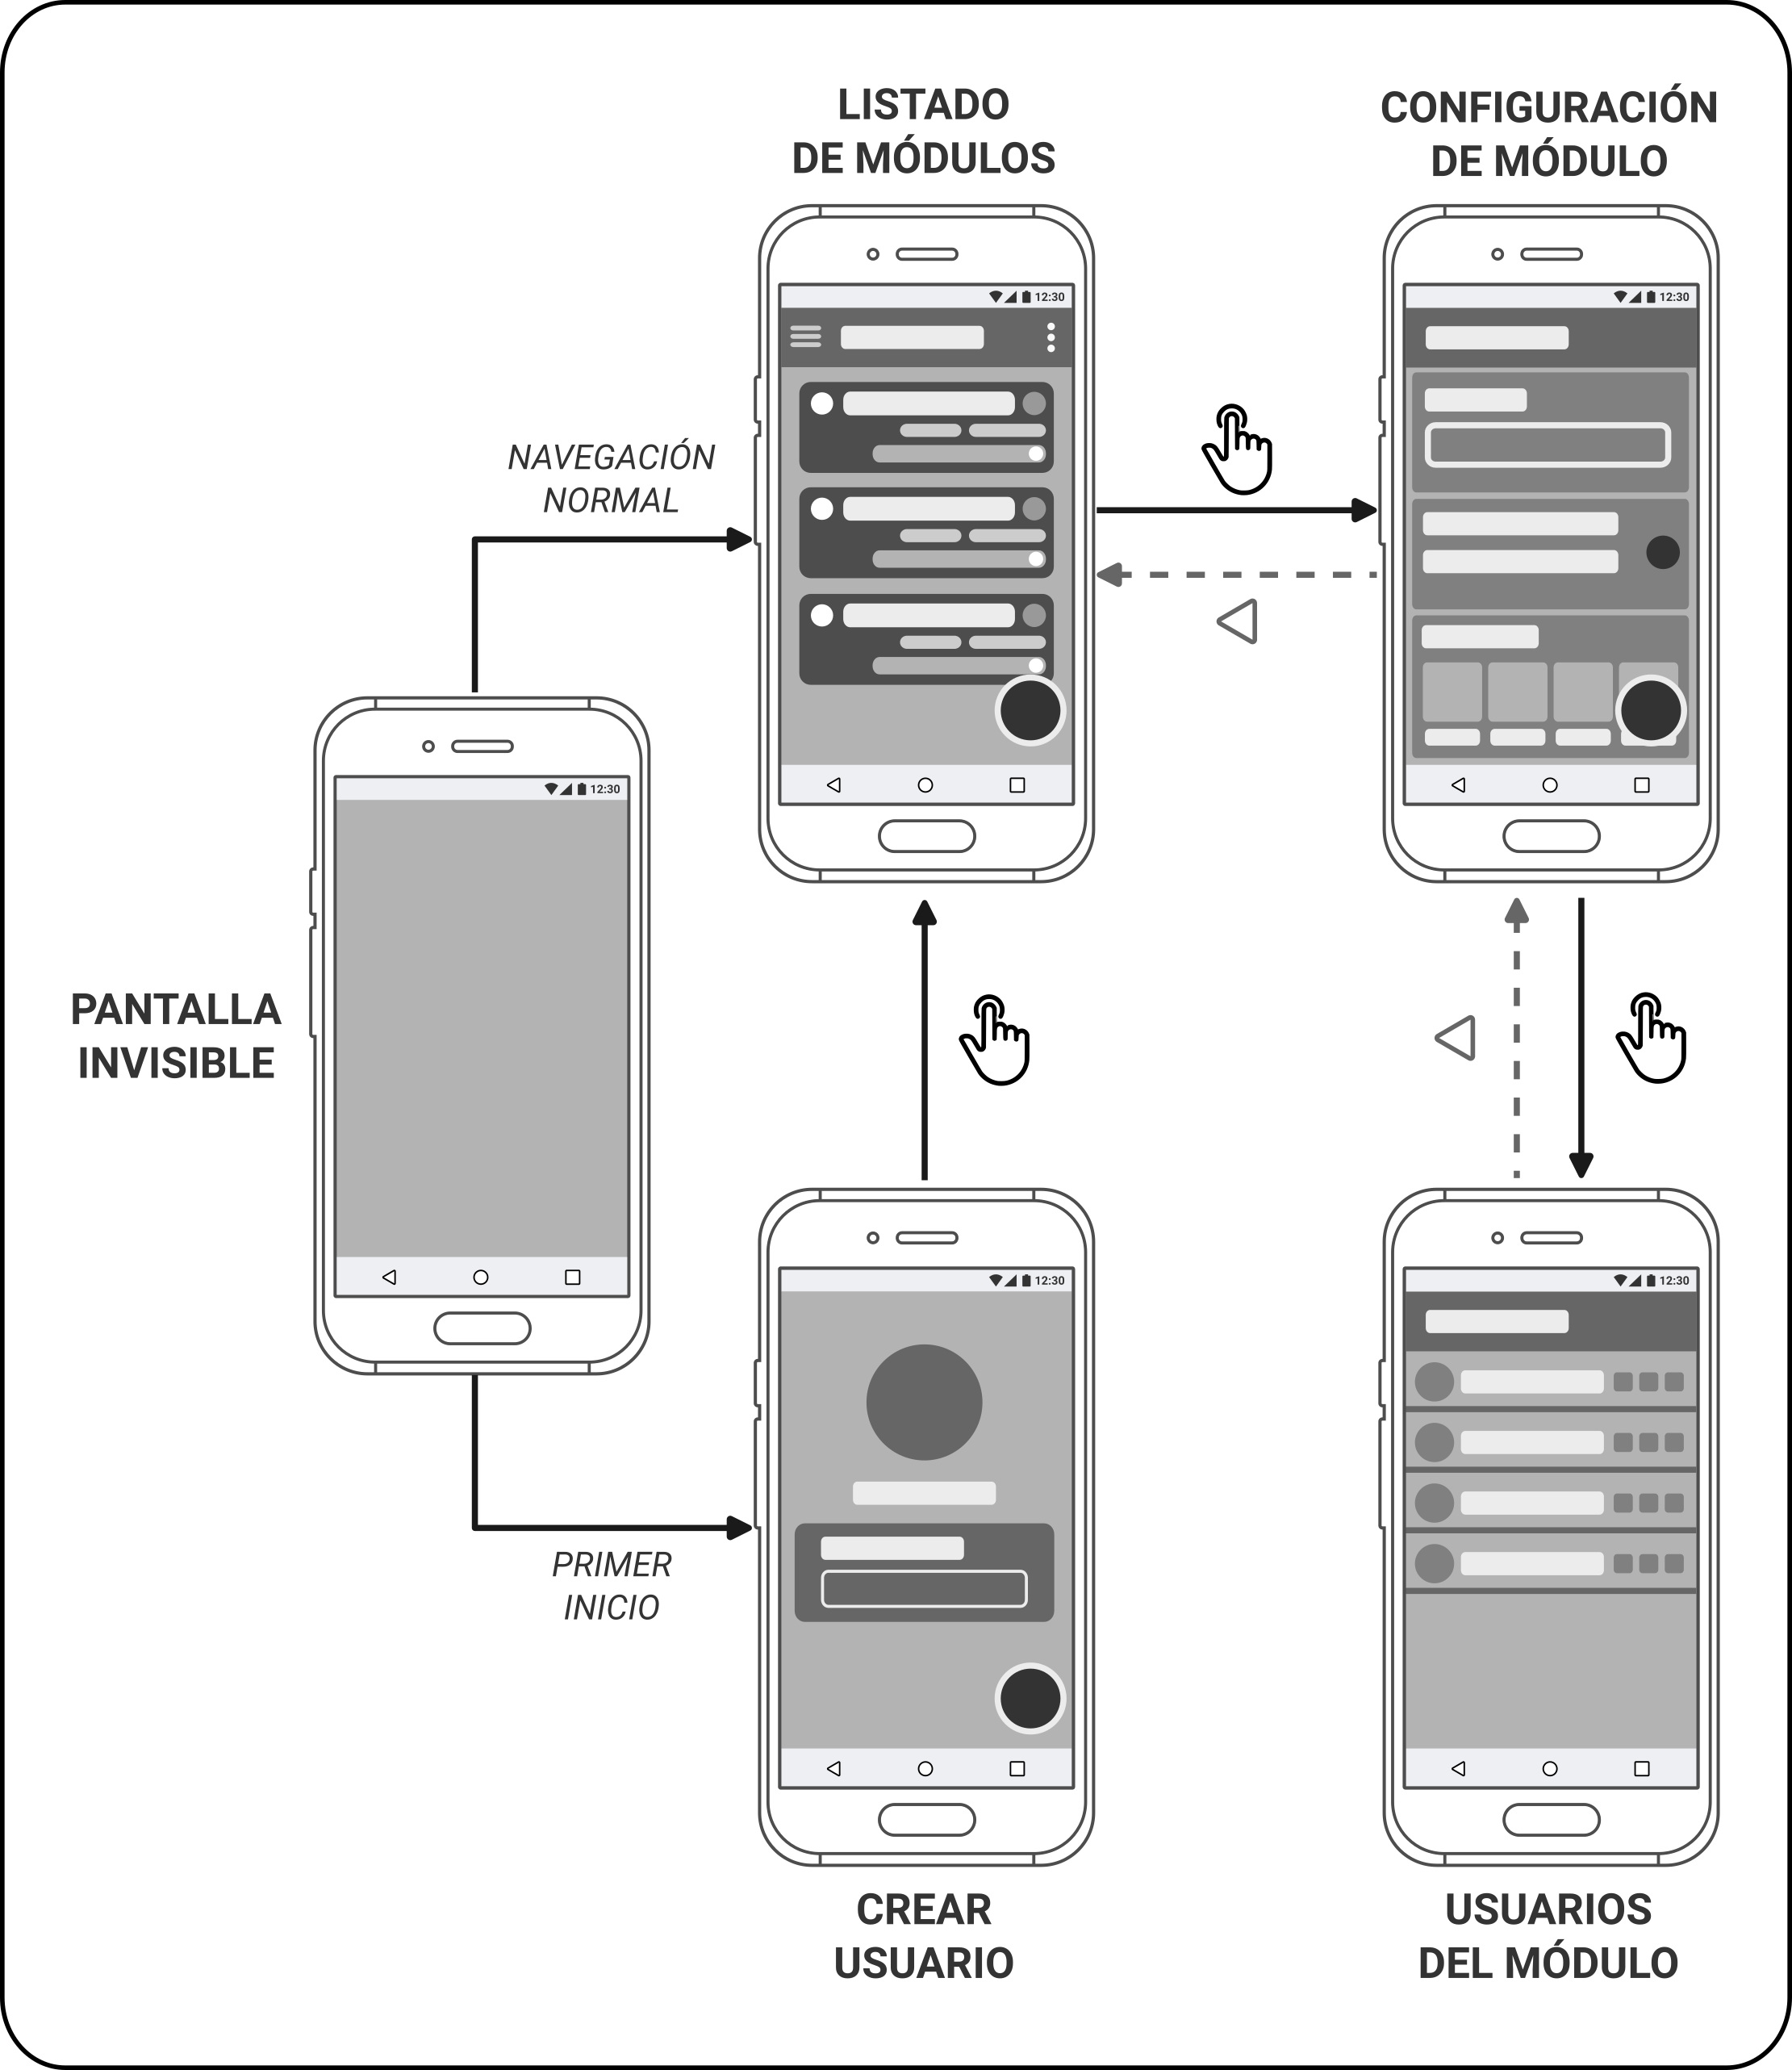
\includegraphics[width=0.8\textwidth]{Figures/design/user_flow_ink.png}
	\rule{35em}{1pt}
	\caption[Diagrama de Navegación (Wireframes)]{Diagrama de flujo de usuario para la aplicación móvil.}
	\label{fig:app_flow}
\end{figure}

Se plantea la definición de unidades funcionales como un conjunto de funcionalidades de la aplicación que están estrechamente relacionadas.
Utilizar las pantallas pareciera una buena estrategia para definir estas unidades. 

\begin{itemize}
	\item \textbf{Creación de Usuario:} El usuario ingresa su número de teléfono y se crea el objeto App User.
	\item \textbf{Listado de Módulos:} Se buscan todos los Módulos disponibles en los distintos canales de comunicación y se muestran en una lista para permitir su manipulación.
	\item \textbf{Configuración del Módulo:} Permite modificar parámetros del módulo seleccionado.
	\item \textbf{Usuarios del Módulo:} Muestra el listado de usuarios de un Módulo y permite su administración.
\end{itemize}

\subsubsection{Plantillas de Arquitectura}
Siguiendo los lineamientos de la arquitectura cada unidad respetará el formato arquitectónico ilustrado en la figura ~\ref{fig:class_unidad}, como puede observarse todos los patrones de diseño están represados en el diagrama de clases. 
\begin{figure}[htbp]
	\centering
	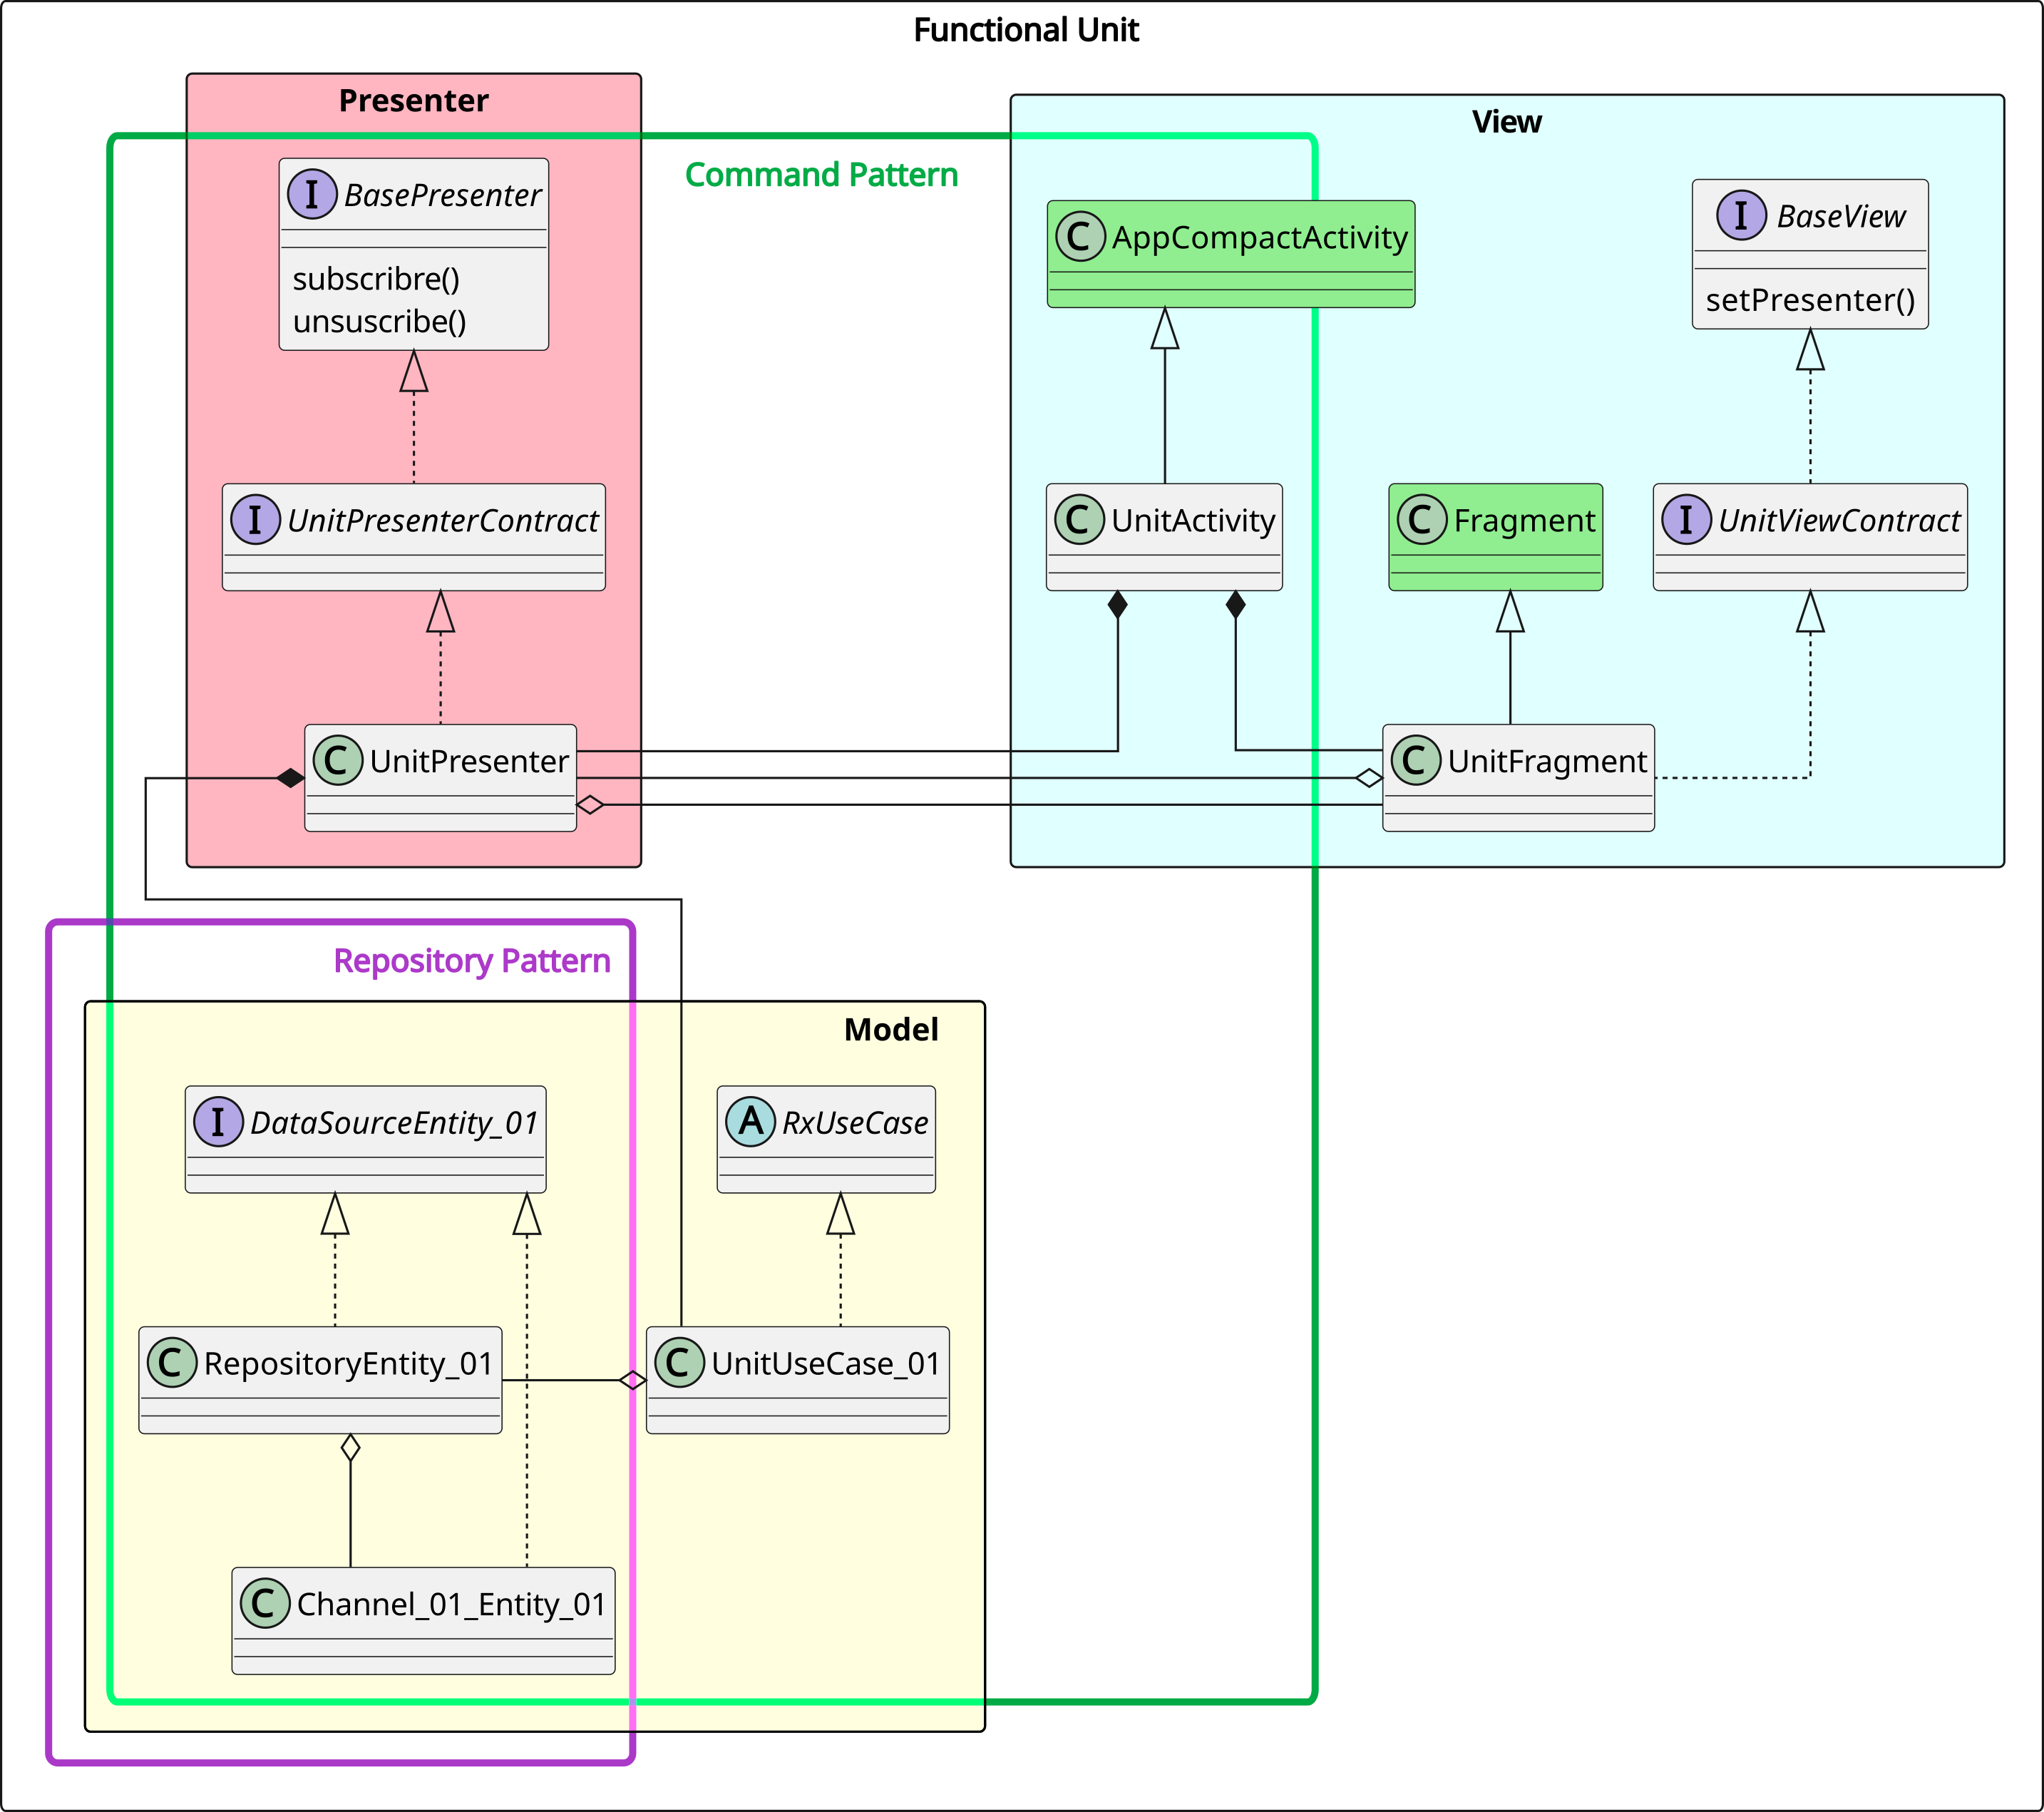
\includegraphics[width=\textwidth]{Figures/design/CLASS_unit_ink.png}
	\rule{35em}{1pt}
	\caption[Clases de Unidad Funcional]{Diagrama de clases de una unidad funcional.}
	\label{fig:class_unidad}
\end{figure}

Al implementar esta plantilla se observa también que la organización del código fuente produce una jerarquía de directorios similar para cada unidad funcional. En la figura ~\ref{fig:dir_unit} se puede observar cómo debería verse cada unidad en el proyecto.

\pagebreak

\begin{multicols}{2}
\begin{Figure}%[b]
	\centering
	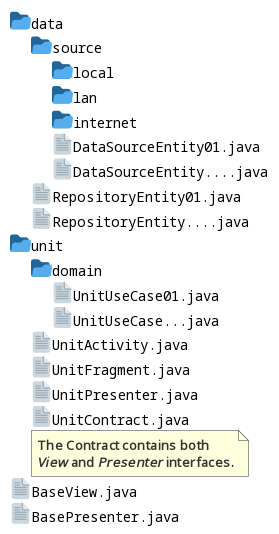
\includegraphics[width=0.8\linewidth]{Figures/design/DIR_generic_unit.png}
	\rule{\linewidth}{1pt}
	\captionof{figure}{Diagrama de directorios de una unidad funcional.}
	\label{fig:dir_unit}
\end{Figure}

\columnbreak % Insert a column break between columns
Un directorio con el nombre de la unidad funcional encapsula los archivos exclusivos de la unidad entre ellos:

Los archivos que implementan la Vista y el Presentador.

En el directorio \texttt{data} se colocan los archivos relacionados con la implementación de los repositorios.

En el directorio \texttt{dominio} estarán los archivos que implementan los casos de uso.
	
\end{multicols}


 
\subsection{Planificación de las Iteraciones}

Para garantizar un prototipo mínimo y plantear las subsecuentes mejoras se proponen tres iteraciones de desarrollo acotadas, consecutivas e incrementales. Con este propósito se definieron tres subconjuntos ~\ref{section:casos_de_uso} sobre los casos de uso documentados en la sección ~\ref{section:casos_de_uso}. Para cada iteración se codificará todo el andamiaje necesario para construir las unidades funcionales con las primitivas de la arquitectura, los repositorios con sus canales correspondientes, el diseño gráfico de las vistas y los algoritmos de los casos de uso.
\pagebreak
\begin{multicols}{2}
	\begin{Figure}%[htbp]
		\centering
		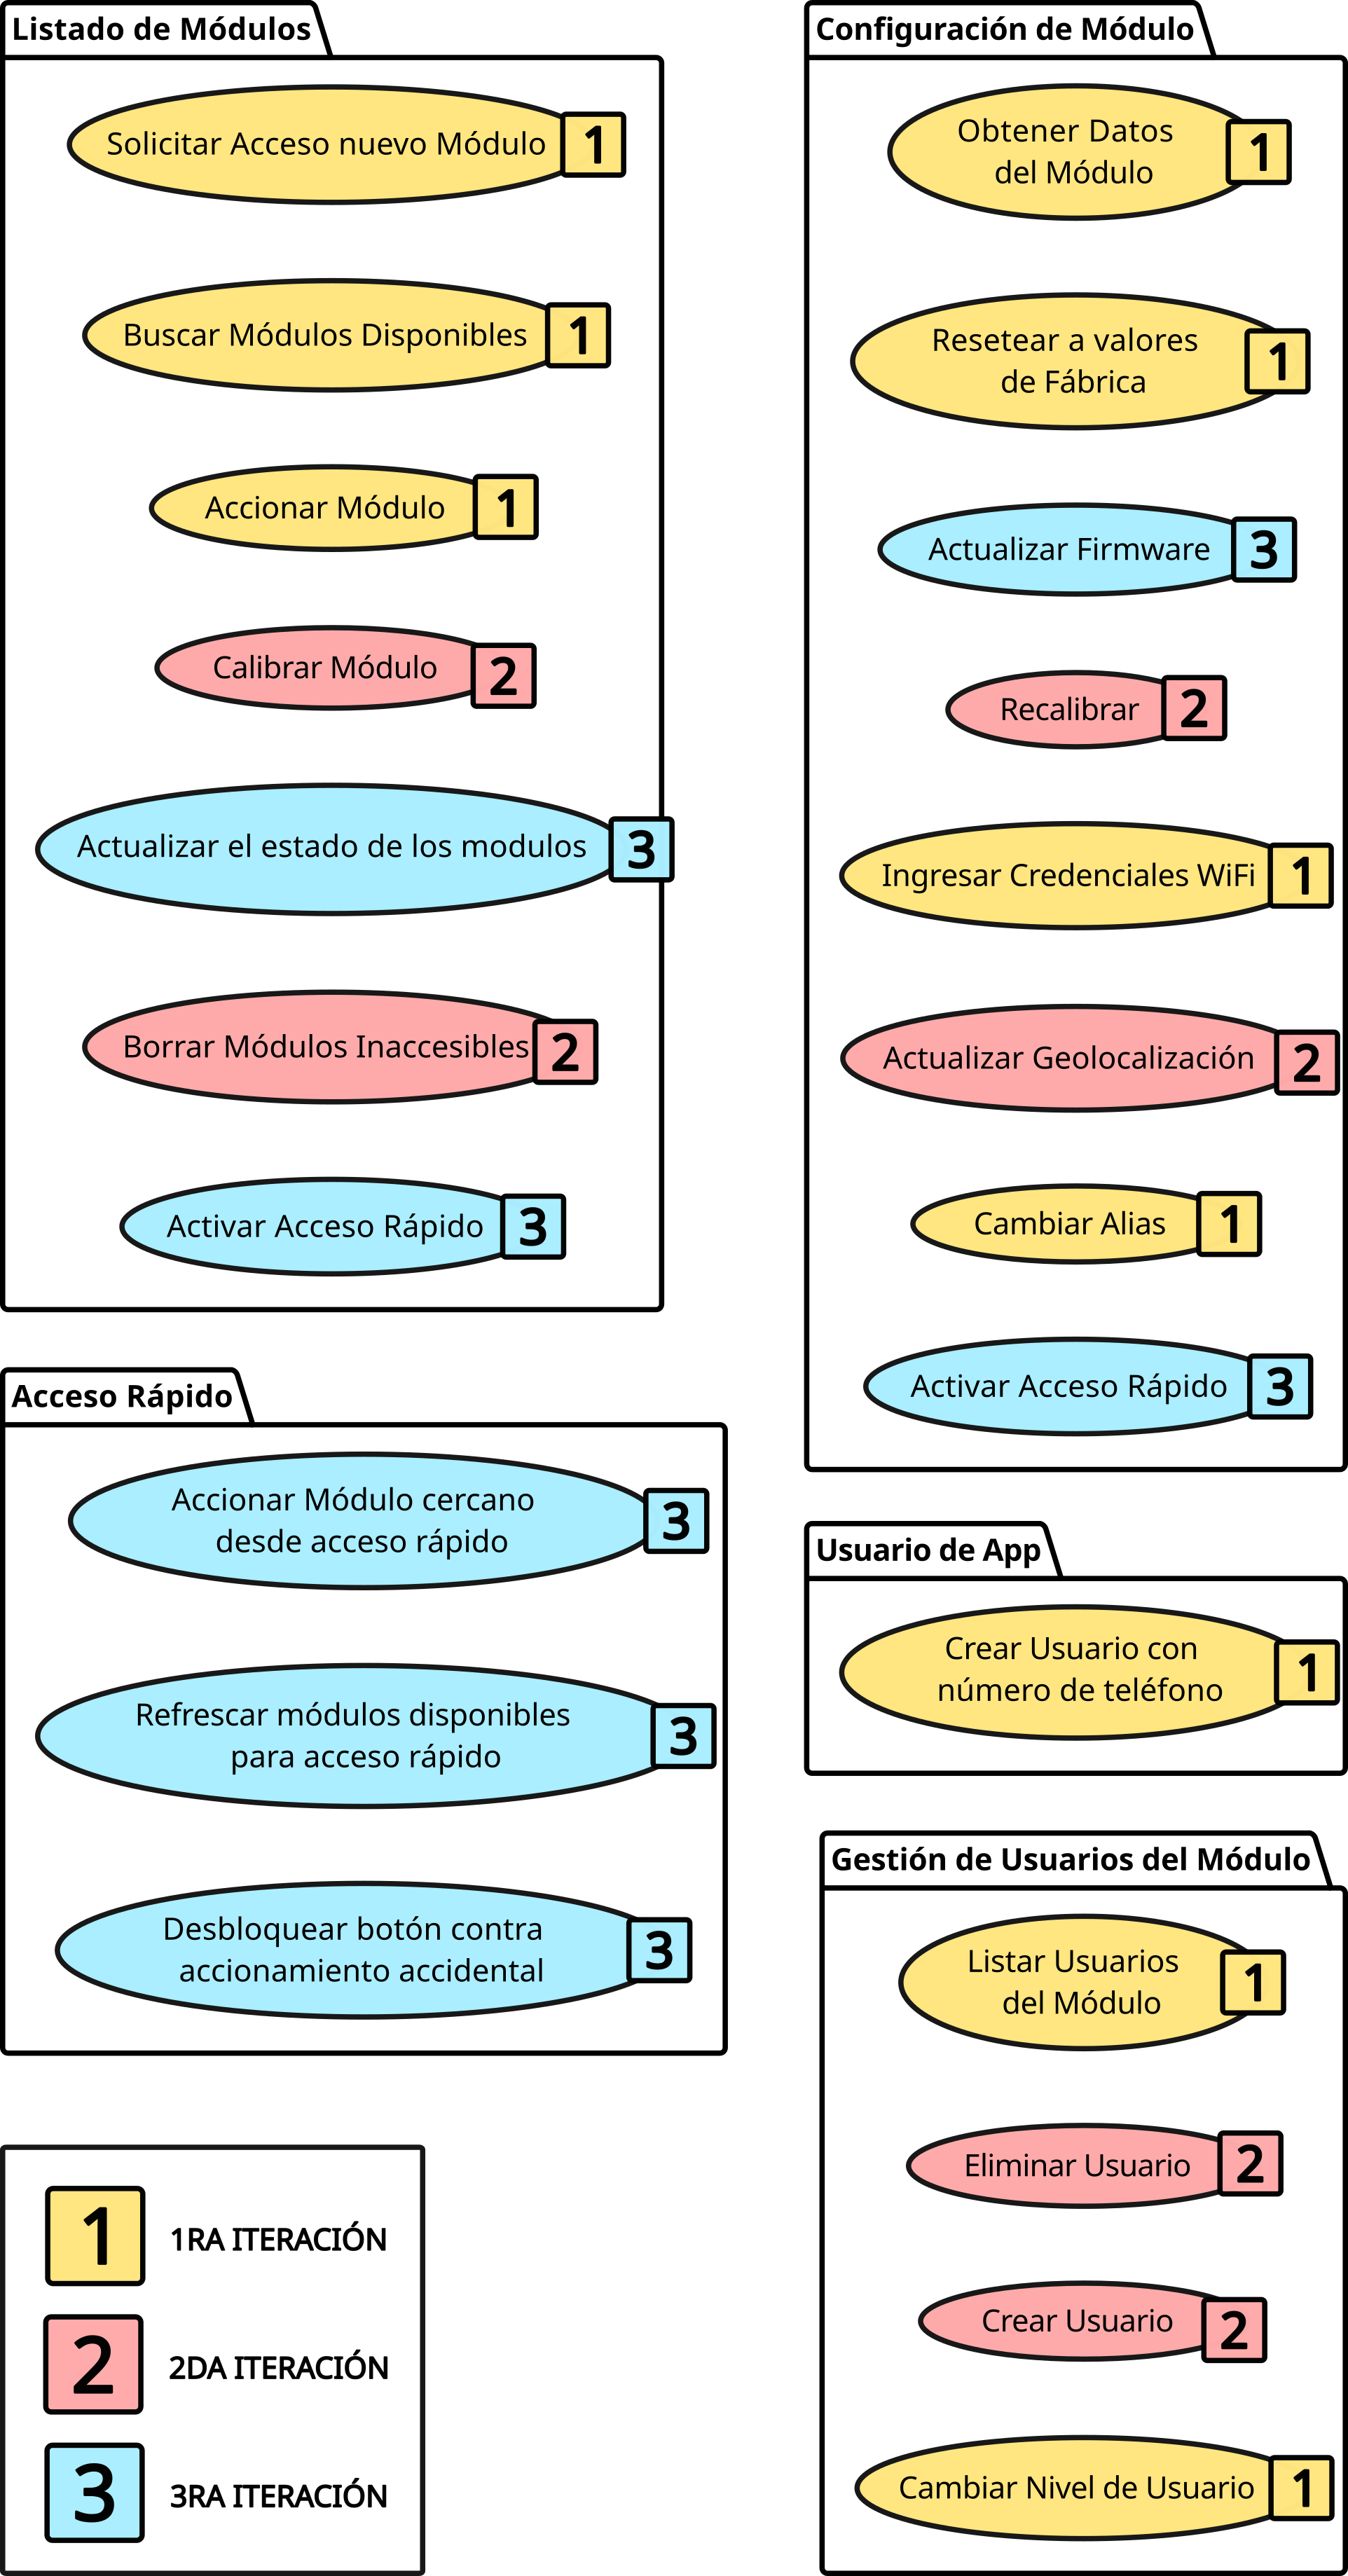
\includegraphics[width=\linewidth]{Figures/design/USE_todos_iterac.png}
		\rule{\linewidth}{1pt}
		\captionof{figure}{Subconjuntos de Casos de Uso para cada Iteración.}
		\label{fig:casosusoiter}
	\end{Figure}
	
	\columnbreak
	Se describe una síntesis del alcance de cada iteración:
	{ \small
	
	\emph{ITERACIÓN I} 
	\begin{itemize}
		\item Se plantea y comenta la implementación reactiva y genérica de un Caso de Uso. Se expondrá sobre el uso y funcionamiento de los Schedulers.
		\item Casos de Uso contemplados para la primera iteración.
		\item El repositorio de los objetos Módulo. Canales de Persistencia local y Comunicación LAN.
	\end{itemize}
	
	
	\emph{ITERACIÓN II}
	\begin{itemize}
		\item Casos de uso contemplados para la segunda iteración.
		\item El repositorio para obtener la ubicación geográfica del teléfono.
		\item Se introducen las pruebas unitarias al código base.
		\item Se configuran, codifican y ejecutan pruebas de interfaz de usuario instrumentadas.
	\end{itemize}

	\emph{ITERACIÓN III}
	\begin{itemize}
		\item Motivación e implementación del ``Control Rápido''.
		\item Casos de uso contemplados para la tercera iteración.
		\item Se documenta la propuesta de comunicación a través de internet.
		\item Wrapper reactivo sobre una librería de terceros.
		\item La lógica de selección de canales disponibles para un mismo repositorio.
		\item Seguridad sobre el canal MQTT.	
	\end{itemize}
	}
\end{multicols}





